\documentclass[twoside]{book}

% Packages required by doxygen
\usepackage{fixltx2e}
\usepackage{calc}
\usepackage{doxygen}
\usepackage[export]{adjustbox} % also loads graphicx
\usepackage{graphicx}
\usepackage[utf8]{inputenc}
\usepackage{makeidx}
\usepackage{multicol}
\usepackage{multirow}
\PassOptionsToPackage{warn}{textcomp}
\usepackage{textcomp}
\usepackage[nointegrals]{wasysym}
\usepackage[table]{xcolor}

% Font selection
\usepackage[T1]{fontenc}
\usepackage[scaled=.90]{helvet}
\usepackage{courier}
\usepackage{amssymb}
\usepackage{sectsty}
\renewcommand{\familydefault}{\sfdefault}
\allsectionsfont{%
  \fontseries{bc}\selectfont%
  \color{darkgray}%
}
\renewcommand{\DoxyLabelFont}{%
  \fontseries{bc}\selectfont%
  \color{darkgray}%
}
\newcommand{\+}{\discretionary{\mbox{\scriptsize$\hookleftarrow$}}{}{}}

% Page & text layout
\usepackage{geometry}
\geometry{%
  a4paper,%
  top=2.5cm,%
  bottom=2.5cm,%
  left=2.5cm,%
  right=2.5cm%
}
\tolerance=750
\hfuzz=15pt
\hbadness=750
\setlength{\emergencystretch}{15pt}
\setlength{\parindent}{0cm}
\setlength{\parskip}{3ex plus 2ex minus 2ex}
\makeatletter
\renewcommand{\paragraph}{%
  \@startsection{paragraph}{4}{0ex}{-1.0ex}{1.0ex}{%
    \normalfont\normalsize\bfseries\SS@parafont%
  }%
}
\renewcommand{\subparagraph}{%
  \@startsection{subparagraph}{5}{0ex}{-1.0ex}{1.0ex}{%
    \normalfont\normalsize\bfseries\SS@subparafont%
  }%
}
\makeatother

% Headers & footers
\usepackage{fancyhdr}
\pagestyle{fancyplain}
\fancyhead[LE]{\fancyplain{}{\bfseries\thepage}}
\fancyhead[CE]{\fancyplain{}{}}
\fancyhead[RE]{\fancyplain{}{\bfseries\leftmark}}
\fancyhead[LO]{\fancyplain{}{\bfseries\rightmark}}
\fancyhead[CO]{\fancyplain{}{}}
\fancyhead[RO]{\fancyplain{}{\bfseries\thepage}}
\fancyfoot[LE]{\fancyplain{}{}}
\fancyfoot[CE]{\fancyplain{}{}}
\fancyfoot[RE]{\fancyplain{}{\bfseries\scriptsize Generated by Doxygen }}
\fancyfoot[LO]{\fancyplain{}{\bfseries\scriptsize Generated by Doxygen }}
\fancyfoot[CO]{\fancyplain{}{}}
\fancyfoot[RO]{\fancyplain{}{}}
\renewcommand{\footrulewidth}{0.4pt}
\renewcommand{\chaptermark}[1]{%
  \markboth{#1}{}%
}
\renewcommand{\sectionmark}[1]{%
  \markright{\thesection\ #1}%
}

% Indices & bibliography
\usepackage{natbib}
\usepackage[titles]{tocloft}
\setcounter{tocdepth}{3}
\setcounter{secnumdepth}{5}
\makeindex

% Hyperlinks (required, but should be loaded last)
\usepackage{ifpdf}
\ifpdf
  \usepackage[pdftex,pagebackref=true]{hyperref}
\else
  \usepackage[ps2pdf,pagebackref=true]{hyperref}
\fi
\hypersetup{%
  colorlinks=true,%
  linkcolor=blue,%
  citecolor=blue,%
  unicode%
}

% Custom commands
\newcommand{\clearemptydoublepage}{%
  \newpage{\pagestyle{empty}\cleardoublepage}%
}

\usepackage{caption}
\captionsetup{labelsep=space,justification=centering,font={bf},singlelinecheck=off,skip=4pt,position=top}

%===== C O N T E N T S =====

\begin{document}

% Titlepage & ToC
\hypersetup{pageanchor=false,
             bookmarksnumbered=true,
             pdfencoding=unicode
            }
\pagenumbering{alph}
\begin{titlepage}
\vspace*{7cm}
\begin{center}%
{\Large Vex Team A \\[1ex]\large 1.\+0.\+1 }\\
\vspace*{1cm}
{\large Generated by Doxygen 1.8.13}\\
\end{center}
\end{titlepage}
\clearemptydoublepage
\pagenumbering{roman}
\tableofcontents
\clearemptydoublepage
\pagenumbering{arabic}
\hypersetup{pageanchor=true}

%--- Begin generated contents ---
\chapter{In\+The\+ZoneA}
\label{md__r_e_a_d_m_e}
\Hypertarget{md__r_e_a_d_m_e}
Team A code for In The Zone 
\chapter{Data Structure Index}
\section{Data Structures}
Here are the data structures with brief descriptions\+:\begin{DoxyCompactList}
\item\contentsline{section}{\hyperlink{structlcd__buttons}{lcd\+\_\+buttons} \\*Repreents the state of the lcd buttons }{\pageref{structlcd__buttons}}{}
\item\contentsline{section}{\hyperlink{structmenu}{menu} }{\pageref{structmenu}}{}
\item\contentsline{section}{\hyperlink{structmenu__result}{menu\+\_\+result} }{\pageref{structmenu__result}}{}
\item\contentsline{section}{\hyperlink{structpolar__cord}{polar\+\_\+cord} \\*A struct that contains polar cordinates }{\pageref{structpolar__cord}}{}
\end{DoxyCompactList}

\chapter{File Index}
\section{File List}
Here is a list of all files with brief descriptions\+:\begin{DoxyCompactList}
\item\contentsline{section}{include/\hyperlink{battery_8h}{battery.\+h} }{\pageref{battery_8h}}{}
\item\contentsline{section}{include/\hyperlink{controller_8h}{controller.\+h} \\*Controller definitions, macros }{\pageref{controller_8h}}{}
\item\contentsline{section}{include/\hyperlink{drive_8h}{drive.\+h} \\*Drive base definitions and enumerations }{\pageref{drive_8h}}{}
\item\contentsline{section}{include/\hyperlink{encoders_8h}{encoders.\+h} \\*Wrapper around encoder functions }{\pageref{encoders_8h}}{}
\item\contentsline{section}{include/\hyperlink{lcd_8h}{lcd.\+h} \\*L\+CD wrapper functions and macros }{\pageref{lcd_8h}}{}
\item\contentsline{section}{include/\hyperlink{log_8h}{log.\+h} \\*Contains logging functions }{\pageref{log_8h}}{}
\item\contentsline{section}{include/\hyperlink{main_8h}{main.\+h} \\*Header file for global functions }{\pageref{main_8h}}{}
\item\contentsline{section}{include/\hyperlink{menu_8h}{menu.\+h} \\*Contains menu functionality and abstraction }{\pageref{menu_8h}}{}
\item\contentsline{section}{include/\hyperlink{ports_8h}{ports.\+h} \\*Port macros for sensors }{\pageref{ports_8h}}{}
\item\contentsline{section}{include/\hyperlink{slew_8h}{slew.\+h} \\*Contains the slew rate controller wrapper for the motors }{\pageref{slew_8h}}{}
\item\contentsline{section}{include/\hyperlink{vlib_8h}{vlib.\+h} \\*Contains misc helpful functions }{\pageref{vlib_8h}}{}
\item\contentsline{section}{include/\hyperlink{vmath_8h}{vmath.\+h} \\*Vex Specific Math Functions, includes\+: Cartesian to polar cordinates }{\pageref{vmath_8h}}{}
\item\contentsline{section}{src/\hyperlink{auto_8c}{auto.\+c} \\*File for autonomous code }{\pageref{auto_8c}}{}
\item\contentsline{section}{src/\hyperlink{battery_8c}{battery.\+c} }{\pageref{battery_8c}}{}
\item\contentsline{section}{src/\hyperlink{controller_8c}{controller.\+c} }{\pageref{controller_8c}}{}
\item\contentsline{section}{src/\hyperlink{drive_8c}{drive.\+c} }{\pageref{drive_8c}}{}
\item\contentsline{section}{src/\hyperlink{encoders_8c}{encoders.\+c} }{\pageref{encoders_8c}}{}
\item\contentsline{section}{src/\hyperlink{init_8c}{init.\+c} \\*File for initialization code }{\pageref{init_8c}}{}
\item\contentsline{section}{src/\hyperlink{lcd_8c}{lcd.\+c} }{\pageref{lcd_8c}}{}
\item\contentsline{section}{src/\hyperlink{log_8c}{log.\+c} }{\pageref{log_8c}}{}
\item\contentsline{section}{src/\hyperlink{menu_8c}{menu.\+c} }{\pageref{menu_8c}}{}
\item\contentsline{section}{src/\hyperlink{opcontrol_8c}{opcontrol.\+c} \\*File for operator control code }{\pageref{opcontrol_8c}}{}
\item\contentsline{section}{src/\hyperlink{slew_8c}{slew.\+c} }{\pageref{slew_8c}}{}
\item\contentsline{section}{src/\hyperlink{vlib_8c}{vlib.\+c} }{\pageref{vlib_8c}}{}
\item\contentsline{section}{src/\hyperlink{vmath_8c}{vmath.\+c} }{\pageref{vmath_8c}}{}
\end{DoxyCompactList}

\chapter{Data Structure Documentation}
\subsection{cord Struct Reference}
\label{structcord}\index{cord@{cord}}


A struct that contains cartesian coordinates.  




{\ttfamily \#include \char`\"{}vmath.\+h\char`\"{}}

\subsubsection*{Data Fields}
\begin{DoxyCompactItemize}
\item 
float \textbf{ x}
\item 
float \textbf{ y}
\end{DoxyCompactItemize}


\subsubsection{Detailed Description}
A struct that contains cartesian coordinates. 

\begin{DoxyDate}{Date}
9/9/2017 
\end{DoxyDate}
\begin{DoxyAuthor}{Author}
Chris Jerrett 
\end{DoxyAuthor}


Definition at line \textbf{ 32} of file \textbf{ vmath.\+h}.



\subsubsection{Field Documentation}
\mbox{\label{structcord_a2eef9b681474b679cf87b0c20eced2cd}} 
\index{cord@{cord}!x@{x}}
\index{x@{x}!cord@{cord}}
\paragraph{x}
{\footnotesize\ttfamily float cord\+::x}

the x coordinate 

Definition at line \textbf{ 34} of file \textbf{ vmath.\+h}.



Referenced by \textbf{ get\+\_\+joystick\+\_\+cord()}, and \textbf{ update\+\_\+drive\+\_\+motors()}.

\mbox{\label{structcord_a4e7d289c55cfe511532e53a81dc19215}} 
\index{cord@{cord}!y@{y}}
\index{y@{y}!cord@{cord}}
\paragraph{y}
{\footnotesize\ttfamily float cord\+::y}

the y coordinate 

Definition at line \textbf{ 36} of file \textbf{ vmath.\+h}.



Referenced by \textbf{ get\+\_\+joystick\+\_\+cord()}, and \textbf{ update\+\_\+drive\+\_\+motors()}.



The documentation for this struct was generated from the following file\+:\begin{DoxyCompactItemize}
\item 
include/\textbf{ vmath.\+h}\end{DoxyCompactItemize}

\section{lcd\+\_\+buttons Struct Reference}
\label{structlcd__buttons}\index{lcd\+\_\+buttons@{lcd\+\_\+buttons}}


represents the state of the lcd buttons  




{\ttfamily \#include $<$lcd.\+h$>$}

\subsection*{Data Fields}
\begin{DoxyCompactItemize}
\item 
\textbf{ button\+\_\+state} \textbf{ left}
\item 
\textbf{ button\+\_\+state} \textbf{ middle}
\item 
\textbf{ button\+\_\+state} \textbf{ right}
\end{DoxyCompactItemize}


\subsection{Detailed Description}
represents the state of the lcd buttons 

\begin{DoxyAuthor}{Author}
Chris Jerrett 
\end{DoxyAuthor}
\begin{DoxyDate}{Date}
9/9/2017 
\end{DoxyDate}


Definition at line \textbf{ 48} of file \textbf{ lcd.\+h}.



\subsection{Field Documentation}
\mbox{\label{structlcd__buttons_ae385efb5ec794acf5f11027f46c6c039}} 
\index{lcd\+\_\+buttons@{lcd\+\_\+buttons}!left@{left}}
\index{left@{left}!lcd\+\_\+buttons@{lcd\+\_\+buttons}}
\subsubsection{left}
{\footnotesize\ttfamily \textbf{ button\+\_\+state} lcd\+\_\+buttons\+::left}



Definition at line \textbf{ 49} of file \textbf{ lcd.\+h}.



Referenced by \textbf{ lcd\+\_\+get\+\_\+pressed\+\_\+buttons()}.

\mbox{\label{structlcd__buttons_a293342810ac56f73979b08f144d6e6b9}} 
\index{lcd\+\_\+buttons@{lcd\+\_\+buttons}!middle@{middle}}
\index{middle@{middle}!lcd\+\_\+buttons@{lcd\+\_\+buttons}}
\subsubsection{middle}
{\footnotesize\ttfamily \textbf{ button\+\_\+state} lcd\+\_\+buttons\+::middle}



Definition at line \textbf{ 50} of file \textbf{ lcd.\+h}.



Referenced by \textbf{ lcd\+\_\+get\+\_\+pressed\+\_\+buttons()}.

\mbox{\label{structlcd__buttons_a2437d744e09ca1bb91ab4ca53ef77198}} 
\index{lcd\+\_\+buttons@{lcd\+\_\+buttons}!right@{right}}
\index{right@{right}!lcd\+\_\+buttons@{lcd\+\_\+buttons}}
\subsubsection{right}
{\footnotesize\ttfamily \textbf{ button\+\_\+state} lcd\+\_\+buttons\+::right}



Definition at line \textbf{ 51} of file \textbf{ lcd.\+h}.



Referenced by \textbf{ lcd\+\_\+get\+\_\+pressed\+\_\+buttons()}.



The documentation for this struct was generated from the following file\+:\begin{DoxyCompactItemize}
\item 
include/\textbf{ lcd.\+h}\end{DoxyCompactItemize}

\subsection{menu\+\_\+t Struct Reference}
\label{structmenu__t}\index{menu\+\_\+t@{menu\+\_\+t}}


Represents a specific instance of a menu. Will cause a memory leak if not deinitialized via denint\+\_\+menu.  




{\ttfamily \#include \char`\"{}menu.\+h\char`\"{}}

\subsubsection*{Data Fields}
\begin{DoxyCompactItemize}
\item 
int \textbf{ current}
\begin{DoxyCompactList}\small\item\em contains the current index of menu. \end{DoxyCompactList}\item 
unsigned int \textbf{ length}
\begin{DoxyCompactList}\small\item\em contains the length of options char$\ast$$\ast$. \end{DoxyCompactList}\item 
int \textbf{ max}
\begin{DoxyCompactList}\small\item\em contains the maximum int value of menu. Defaults to minimum int value \end{DoxyCompactList}\item 
float \textbf{ max\+\_\+f}
\begin{DoxyCompactList}\small\item\em contains the maximum float value of menu. Defaults to minimum int value \end{DoxyCompactList}\item 
int \textbf{ min}
\begin{DoxyCompactList}\small\item\em contains the minimum int value of menu. Defaults to minimum int value \end{DoxyCompactList}\item 
float \textbf{ min\+\_\+f}
\begin{DoxyCompactList}\small\item\em contains the minimum float value of menu. Defaults to minimum int value \end{DoxyCompactList}\item 
char $\ast$$\ast$ \textbf{ options}
\begin{DoxyCompactList}\small\item\em contains the array of string options. \end{DoxyCompactList}\item 
char $\ast$ \textbf{ prompt}
\begin{DoxyCompactList}\small\item\em contains the prompt to display on the first line. Step is how much the int menu will increase of decrease with each press. Defaults to one \end{DoxyCompactList}\item 
int \textbf{ step}
\begin{DoxyCompactList}\small\item\em contains the step int value of menu. Step is how much the int menu will increase of decrease with each press. Defaults to one \end{DoxyCompactList}\item 
float \textbf{ step\+\_\+f}
\begin{DoxyCompactList}\small\item\em contains the step float value of menu. Step is how much the int menu will increase of decrease with each press. Defaults to 1.\+0f \end{DoxyCompactList}\item 
enum \textbf{ menu\+\_\+type} \textbf{ type}
\begin{DoxyCompactList}\small\item\em contains the type of menu. \end{DoxyCompactList}\end{DoxyCompactItemize}


\subsubsection{Detailed Description}
Represents a specific instance of a menu. Will cause a memory leak if not deinitialized via denint\+\_\+menu. 

\begin{DoxyAuthor}{Author}
Chris Jerrett 
\end{DoxyAuthor}
\begin{DoxyDate}{Date}
9/8/17 
\end{DoxyDate}
\begin{DoxySeeAlso}{See also}
\doxyref{menu.\+h}{p.}{menu_8h} 

\doxyref{menu\+\_\+t}{p.}{structmenu__t} 

\doxyref{create\+\_\+menu}{p.}{menu_8c_aff4fd27ff7707295d91c67fa52a6b021} 

init\+\_\+menu 

\doxyref{display\+\_\+menu}{p.}{menu_8c_abfadedb104f89f672dd3045499975a71} 

\doxyref{menu\+\_\+type}{p.}{menu_8h_a6bbf4baf5018b0d76aab6c2e6bf85e62} 

\doxyref{denint\+\_\+menu}{p.}{menu_8c_a05a36619ac6c9ba4544eddb83ee2a50d} 
\end{DoxySeeAlso}


Definition at line \textbf{ 66} of file \textbf{ menu.\+h}.



\subsubsection{Field Documentation}
\mbox{\label{structmenu__t_a2acb18066898677ec5e2dc40eec811c5}} 
\index{menu\+\_\+t@{menu\+\_\+t}!current@{current}}
\index{current@{current}!menu\+\_\+t@{menu\+\_\+t}}
\paragraph{current}
{\footnotesize\ttfamily int menu\+\_\+t\+::current}



contains the current index of menu. 

\begin{DoxyAuthor}{Author}
Chris Jerrett 
\end{DoxyAuthor}
\begin{DoxyDate}{Date}
9/8/17 
\end{DoxyDate}


Definition at line \textbf{ 140} of file \textbf{ menu.\+h}.



Referenced by \textbf{ calculate\+\_\+current\+\_\+display()}, and \textbf{ display\+\_\+menu()}.

\mbox{\label{structmenu__t_a023063461c4a247e574abd6a55faf765}} 
\index{menu\+\_\+t@{menu\+\_\+t}!length@{length}}
\index{length@{length}!menu\+\_\+t@{menu\+\_\+t}}
\paragraph{length}
{\footnotesize\ttfamily unsigned int menu\+\_\+t\+::length}



contains the length of options char$\ast$$\ast$. 

\begin{DoxyAuthor}{Author}
Chris Jerrett 
\end{DoxyAuthor}
\begin{DoxyDate}{Date}
9/8/17 
\end{DoxyDate}


Definition at line \textbf{ 86} of file \textbf{ menu.\+h}.



Referenced by \textbf{ calculate\+\_\+current\+\_\+display()}, and \textbf{ init\+\_\+menu\+\_\+var()}.

\mbox{\label{structmenu__t_ace9cbaecd7bf311be0ef230da657f406}} 
\index{menu\+\_\+t@{menu\+\_\+t}!max@{max}}
\index{max@{max}!menu\+\_\+t@{menu\+\_\+t}}
\paragraph{max}
{\footnotesize\ttfamily int menu\+\_\+t\+::max}



contains the maximum int value of menu. Defaults to minimum int value 

\begin{DoxyAuthor}{Author}
Chris Jerrett 
\end{DoxyAuthor}
\begin{DoxyDate}{Date}
9/8/17 
\end{DoxyDate}


Definition at line \textbf{ 102} of file \textbf{ menu.\+h}.



Referenced by \textbf{ calculate\+\_\+current\+\_\+display()}, \textbf{ create\+\_\+menu()}, and \textbf{ init\+\_\+menu\+\_\+int()}.

\mbox{\label{structmenu__t_a14b11d0a7610484462c8a6e93068a2c1}} 
\index{menu\+\_\+t@{menu\+\_\+t}!max\+\_\+f@{max\+\_\+f}}
\index{max\+\_\+f@{max\+\_\+f}!menu\+\_\+t@{menu\+\_\+t}}
\paragraph{max\+\_\+f}
{\footnotesize\ttfamily float menu\+\_\+t\+::max\+\_\+f}



contains the maximum float value of menu. Defaults to minimum int value 

\begin{DoxyAuthor}{Author}
Chris Jerrett 
\end{DoxyAuthor}
\begin{DoxyDate}{Date}
9/8/17 
\end{DoxyDate}


Definition at line \textbf{ 126} of file \textbf{ menu.\+h}.



Referenced by \textbf{ calculate\+\_\+current\+\_\+display()}, \textbf{ create\+\_\+menu()}, and \textbf{ init\+\_\+menu\+\_\+float()}.

\mbox{\label{structmenu__t_a6891bc6c94f1e995cc62a05b13328de5}} 
\index{menu\+\_\+t@{menu\+\_\+t}!min@{min}}
\index{min@{min}!menu\+\_\+t@{menu\+\_\+t}}
\paragraph{min}
{\footnotesize\ttfamily int menu\+\_\+t\+::min}



contains the minimum int value of menu. Defaults to minimum int value 

\begin{DoxyAuthor}{Author}
Chris Jerrett 
\end{DoxyAuthor}
\begin{DoxyDate}{Date}
9/8/17 
\end{DoxyDate}


Definition at line \textbf{ 94} of file \textbf{ menu.\+h}.



Referenced by \textbf{ calculate\+\_\+current\+\_\+display()}, \textbf{ create\+\_\+menu()}, and \textbf{ init\+\_\+menu\+\_\+int()}.

\mbox{\label{structmenu__t_a0a6e4f711992fb69e8a57c2af1ab7a05}} 
\index{menu\+\_\+t@{menu\+\_\+t}!min\+\_\+f@{min\+\_\+f}}
\index{min\+\_\+f@{min\+\_\+f}!menu\+\_\+t@{menu\+\_\+t}}
\paragraph{min\+\_\+f}
{\footnotesize\ttfamily float menu\+\_\+t\+::min\+\_\+f}



contains the minimum float value of menu. Defaults to minimum int value 

\begin{DoxyAuthor}{Author}
Chris Jerrett 
\end{DoxyAuthor}
\begin{DoxyDate}{Date}
9/8/17 
\end{DoxyDate}


Definition at line \textbf{ 118} of file \textbf{ menu.\+h}.



Referenced by \textbf{ calculate\+\_\+current\+\_\+display()}, \textbf{ create\+\_\+menu()}, and \textbf{ init\+\_\+menu\+\_\+float()}.

\mbox{\label{structmenu__t_ad695cd88051e34817f0f582d4e43c33a}} 
\index{menu\+\_\+t@{menu\+\_\+t}!options@{options}}
\index{options@{options}!menu\+\_\+t@{menu\+\_\+t}}
\paragraph{options}
{\footnotesize\ttfamily char$\ast$$\ast$ menu\+\_\+t\+::options}



contains the array of string options. 

\begin{DoxyAuthor}{Author}
Chris Jerrett 
\end{DoxyAuthor}
\begin{DoxyDate}{Date}
9/8/17 
\end{DoxyDate}


Definition at line \textbf{ 79} of file \textbf{ menu.\+h}.



Referenced by \textbf{ calculate\+\_\+current\+\_\+display()}, \textbf{ denint\+\_\+menu()}, and \textbf{ init\+\_\+menu\+\_\+var()}.

\mbox{\label{structmenu__t_a7bf29a030b7ed4a623c6b445587cc647}} 
\index{menu\+\_\+t@{menu\+\_\+t}!prompt@{prompt}}
\index{prompt@{prompt}!menu\+\_\+t@{menu\+\_\+t}}
\paragraph{prompt}
{\footnotesize\ttfamily char$\ast$ menu\+\_\+t\+::prompt}



contains the prompt to display on the first line. Step is how much the int menu will increase of decrease with each press. Defaults to one 

\begin{DoxyAuthor}{Author}
Chris Jerrett 
\end{DoxyAuthor}
\begin{DoxyDate}{Date}
9/8/17 
\end{DoxyDate}


Definition at line \textbf{ 147} of file \textbf{ menu.\+h}.



Referenced by \textbf{ create\+\_\+menu()}, \textbf{ denint\+\_\+menu()}, and \textbf{ display\+\_\+menu()}.

\mbox{\label{structmenu__t_adc50450bc59ea66a8d67424adc46e24e}} 
\index{menu\+\_\+t@{menu\+\_\+t}!step@{step}}
\index{step@{step}!menu\+\_\+t@{menu\+\_\+t}}
\paragraph{step}
{\footnotesize\ttfamily int menu\+\_\+t\+::step}



contains the step int value of menu. Step is how much the int menu will increase of decrease with each press. Defaults to one 

\begin{DoxyAuthor}{Author}
Chris Jerrett 
\end{DoxyAuthor}
\begin{DoxyDate}{Date}
9/8/17 
\end{DoxyDate}


Definition at line \textbf{ 110} of file \textbf{ menu.\+h}.



Referenced by \textbf{ calculate\+\_\+current\+\_\+display()}, \textbf{ create\+\_\+menu()}, and \textbf{ init\+\_\+menu\+\_\+int()}.

\mbox{\label{structmenu__t_a84cfd9226f6554c63ca9f4b11f94d12d}} 
\index{menu\+\_\+t@{menu\+\_\+t}!step\+\_\+f@{step\+\_\+f}}
\index{step\+\_\+f@{step\+\_\+f}!menu\+\_\+t@{menu\+\_\+t}}
\paragraph{step\+\_\+f}
{\footnotesize\ttfamily float menu\+\_\+t\+::step\+\_\+f}



contains the step float value of menu. Step is how much the int menu will increase of decrease with each press. Defaults to 1.\+0f 

\begin{DoxyAuthor}{Author}
Chris Jerrett 
\end{DoxyAuthor}
\begin{DoxyDate}{Date}
9/8/17 
\end{DoxyDate}


Definition at line \textbf{ 134} of file \textbf{ menu.\+h}.



Referenced by \textbf{ calculate\+\_\+current\+\_\+display()}, \textbf{ create\+\_\+menu()}, and \textbf{ init\+\_\+menu\+\_\+float()}.

\mbox{\label{structmenu__t_a110244ceb7d2a7cba95cfc5758d61c01}} 
\index{menu\+\_\+t@{menu\+\_\+t}!type@{type}}
\index{type@{type}!menu\+\_\+t@{menu\+\_\+t}}
\paragraph{type}
{\footnotesize\ttfamily enum \textbf{ menu\+\_\+type} menu\+\_\+t\+::type}



contains the type of menu. 

\begin{DoxyAuthor}{Author}
Chris Jerrett 
\end{DoxyAuthor}
\begin{DoxyDate}{Date}
9/8/17 
\end{DoxyDate}


Definition at line \textbf{ 72} of file \textbf{ menu.\+h}.



Referenced by \textbf{ calculate\+\_\+current\+\_\+display()}, and \textbf{ create\+\_\+menu()}.



The documentation for this struct was generated from the following file\+:\begin{DoxyCompactItemize}
\item 
include/\textbf{ menu.\+h}\end{DoxyCompactItemize}

\hypertarget{structpolar__cord}{}\section{polar\+\_\+cord Struct Reference}
\label{structpolar__cord}\index{polar\+\_\+cord@{polar\+\_\+cord}}


A struct that contains polar coordinates.  




{\ttfamily \#include $<$vmath.\+h$>$}

\subsection*{Data Fields}
\begin{DoxyCompactItemize}
\item 
float \hyperlink{structpolar__cord_a81b3a11d38d76719b02fcd425adaa216}{angle}
\item 
float \hyperlink{structpolar__cord_aec2e25fecc82af176f0fcd23f1e02f0c}{magnitue}
\end{DoxyCompactItemize}


\subsection{Detailed Description}
A struct that contains polar coordinates. 

\begin{DoxyDate}{Date}
9/9/2017 
\end{DoxyDate}
\begin{DoxyAuthor}{Author}
Chris Jerrett 
\end{DoxyAuthor}


Definition at line 20 of file vmath.\+h.



\subsection{Field Documentation}
\mbox{\Hypertarget{structpolar__cord_a81b3a11d38d76719b02fcd425adaa216}\label{structpolar__cord_a81b3a11d38d76719b02fcd425adaa216}} 
\index{polar\+\_\+cord@{polar\+\_\+cord}!angle@{angle}}
\index{angle@{angle}!polar\+\_\+cord@{polar\+\_\+cord}}
\subsubsection{\texorpdfstring{angle}{angle}}
{\footnotesize\ttfamily float polar\+\_\+cord\+::angle}

the angle of the vector 

Definition at line 22 of file vmath.\+h.



Referenced by cartesian\+\_\+to\+\_\+polar().

\mbox{\Hypertarget{structpolar__cord_aec2e25fecc82af176f0fcd23f1e02f0c}\label{structpolar__cord_aec2e25fecc82af176f0fcd23f1e02f0c}} 
\index{polar\+\_\+cord@{polar\+\_\+cord}!magnitue@{magnitue}}
\index{magnitue@{magnitue}!polar\+\_\+cord@{polar\+\_\+cord}}
\subsubsection{\texorpdfstring{magnitue}{magnitue}}
{\footnotesize\ttfamily float polar\+\_\+cord\+::magnitue}

the magnitude of the vector 

Definition at line 24 of file vmath.\+h.



Referenced by cartesian\+\_\+to\+\_\+polar().



The documentation for this struct was generated from the following file\+:\begin{DoxyCompactItemize}
\item 
include/\hyperlink{vmath_8h}{vmath.\+h}\end{DoxyCompactItemize}

\chapter{File Documentation}
\subsection{include/battery.h File Reference}
\label{battery_8h}\index{include/battery.\+h@{include/battery.\+h}}


Battery management related functions.  


\subsubsection*{Functions}
\begin{DoxyCompactItemize}
\item 
double \textbf{ backup\+\_\+battery\+\_\+voltage} ()
\begin{DoxyCompactList}\small\item\em gets the backup battery voltage \end{DoxyCompactList}\item 
bool \textbf{ battery\+\_\+level\+\_\+acceptable} ()
\begin{DoxyCompactList}\small\item\em returns if the batteries are acceptable \end{DoxyCompactList}\item 
double \textbf{ main\+\_\+battery\+\_\+voltage} ()
\begin{DoxyCompactList}\small\item\em gets the main battery voltage \end{DoxyCompactList}\end{DoxyCompactItemize}


\subsubsection{Detailed Description}
Battery management related functions. 

\begin{DoxyAuthor}{Author}
Chris Jerrett 
\end{DoxyAuthor}
\begin{DoxyDate}{Date}
9/18/2017 
\end{DoxyDate}


Definition in file \textbf{ battery.\+h}.



\subsubsection{Function Documentation}
\mbox{\label{battery_8h_a9b1c5cf7ddddebf63796050a1d4a9969}} 
\index{battery.\+h@{battery.\+h}!backup\+\_\+battery\+\_\+voltage@{backup\+\_\+battery\+\_\+voltage}}
\index{backup\+\_\+battery\+\_\+voltage@{backup\+\_\+battery\+\_\+voltage}!battery.\+h@{battery.\+h}}
\paragraph{backup\+\_\+battery\+\_\+voltage()}
{\footnotesize\ttfamily double backup\+\_\+battery\+\_\+voltage (\begin{DoxyParamCaption}{ }\end{DoxyParamCaption})}



gets the backup battery voltage 

\begin{DoxyAuthor}{Author}
Chris Jerrett 
\end{DoxyAuthor}


Definition at line \textbf{ 14} of file \textbf{ battery.\+c}.



References \textbf{ power\+Level\+Backup()}.



Referenced by \textbf{ battery\+\_\+level\+\_\+acceptable()}.


\begin{DoxyCode}
00014 \{ \textcolor{keywordflow}{return} powerLevelBackup() / 1000.0; \}
\end{DoxyCode}
Here is the call graph for this function\+:
\nopagebreak
\begin{figure}[H]
\begin{center}
\leavevmode
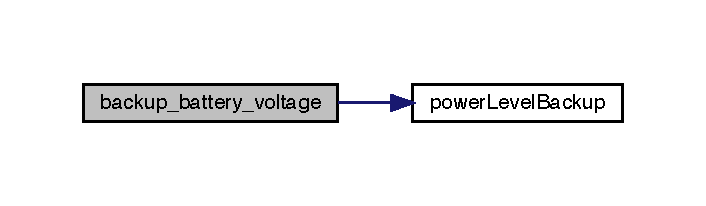
\includegraphics[width=339pt]{battery_8h_a9b1c5cf7ddddebf63796050a1d4a9969_cgraph}
\end{center}
\end{figure}
Here is the caller graph for this function\+:
\nopagebreak
\begin{figure}[H]
\begin{center}
\leavevmode
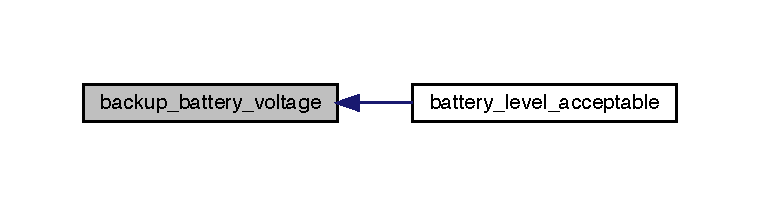
\includegraphics[width=350pt]{battery_8h_a9b1c5cf7ddddebf63796050a1d4a9969_icgraph}
\end{center}
\end{figure}
\mbox{\label{battery_8h_a1097bbb878f6e2690f8eea6cd231959a}} 
\index{battery.\+h@{battery.\+h}!battery\+\_\+level\+\_\+acceptable@{battery\+\_\+level\+\_\+acceptable}}
\index{battery\+\_\+level\+\_\+acceptable@{battery\+\_\+level\+\_\+acceptable}!battery.\+h@{battery.\+h}}
\paragraph{battery\+\_\+level\+\_\+acceptable()}
{\footnotesize\ttfamily bool battery\+\_\+level\+\_\+acceptable (\begin{DoxyParamCaption}{ }\end{DoxyParamCaption})}



returns if the batteries are acceptable 

\begin{DoxySeeAlso}{See also}
M\+I\+N\+\_\+\+M\+A\+I\+N\+\_\+\+V\+O\+L\+T\+A\+GE 

M\+I\+N\+\_\+\+B\+A\+C\+K\+U\+P\+\_\+\+V\+O\+L\+T\+A\+GE
\end{DoxySeeAlso}
\begin{DoxyAuthor}{Author}
Chris Jerrett 
\end{DoxyAuthor}


Definition at line \textbf{ 23} of file \textbf{ battery.\+c}.



References \textbf{ backup\+\_\+battery\+\_\+voltage()}, and \textbf{ main\+\_\+battery\+\_\+voltage()}.



Referenced by \textbf{ initialize()}.


\begin{DoxyCode}
00023                                 \{
00024   \textcolor{keywordflow}{if} (main_battery_voltage() < MIN\_MAIN\_VOLTAGE)
00025     \textcolor{keywordflow}{return} \textcolor{keyword}{false};
00026   \textcolor{keywordflow}{if} (backup_battery_voltage() < MIN\_BACKUP\_VOLTAGE)
00027     \textcolor{keywordflow}{return} \textcolor{keyword}{false};
00028   \textcolor{keywordflow}{return} \textcolor{keyword}{true};
00029 \}
\end{DoxyCode}
Here is the call graph for this function\+:
\nopagebreak
\begin{figure}[H]
\begin{center}
\leavevmode
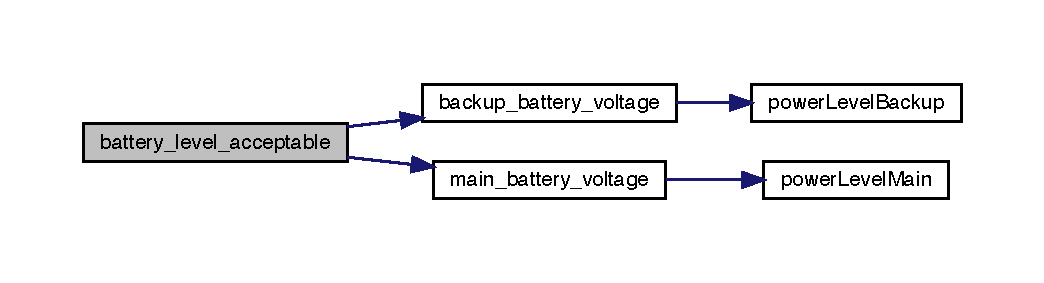
\includegraphics[width=350pt]{battery_8h_a1097bbb878f6e2690f8eea6cd231959a_cgraph}
\end{center}
\end{figure}
Here is the caller graph for this function\+:
\nopagebreak
\begin{figure}[H]
\begin{center}
\leavevmode
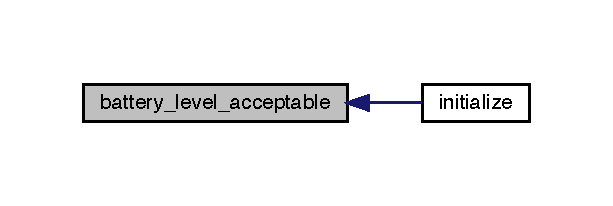
\includegraphics[width=294pt]{battery_8h_a1097bbb878f6e2690f8eea6cd231959a_icgraph}
\end{center}
\end{figure}
\mbox{\label{battery_8h_a8c92c389534fdb079698cdebeb7f2efa}} 
\index{battery.\+h@{battery.\+h}!main\+\_\+battery\+\_\+voltage@{main\+\_\+battery\+\_\+voltage}}
\index{main\+\_\+battery\+\_\+voltage@{main\+\_\+battery\+\_\+voltage}!battery.\+h@{battery.\+h}}
\paragraph{main\+\_\+battery\+\_\+voltage()}
{\footnotesize\ttfamily double main\+\_\+battery\+\_\+voltage (\begin{DoxyParamCaption}{ }\end{DoxyParamCaption})}



gets the main battery voltage 

\begin{DoxyAuthor}{Author}
Chris Jerrett 
\end{DoxyAuthor}


Definition at line \textbf{ 8} of file \textbf{ battery.\+c}.



References \textbf{ power\+Level\+Main()}.



Referenced by \textbf{ battery\+\_\+level\+\_\+acceptable()}.


\begin{DoxyCode}
00008 \{ \textcolor{keywordflow}{return} powerLevelMain() / 1000.0; \}
\end{DoxyCode}
Here is the call graph for this function\+:
\nopagebreak
\begin{figure}[H]
\begin{center}
\leavevmode
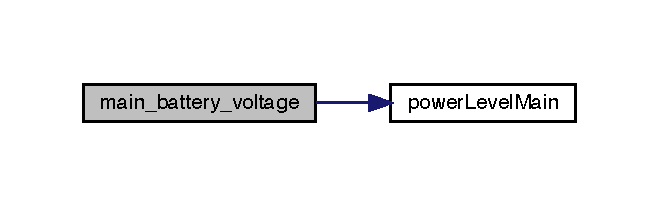
\includegraphics[width=316pt]{battery_8h_a8c92c389534fdb079698cdebeb7f2efa_cgraph}
\end{center}
\end{figure}
Here is the caller graph for this function\+:
\nopagebreak
\begin{figure}[H]
\begin{center}
\leavevmode
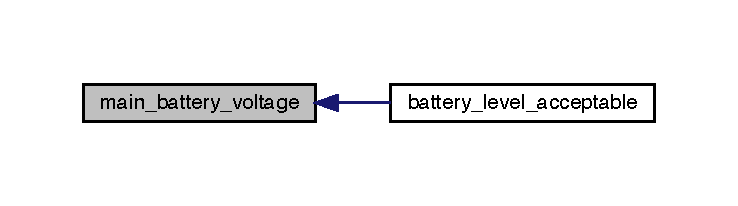
\includegraphics[width=350pt]{battery_8h_a8c92c389534fdb079698cdebeb7f2efa_icgraph}
\end{center}
\end{figure}

\section{include/controller.h File Reference}
\label{controller_8h}\index{include/controller.\+h@{include/controller.\+h}}


controller definitions, macros and functions to assist with usig the vex controllers.  


{\ttfamily \#include \char`\"{}vmath.\+h\char`\"{}}\newline
{\ttfamily \#include $<$A\+P\+I.\+h$>$}\newline
Include dependency graph for controller.\+h\+:\nopagebreak
\begin{figure}[H]
\begin{center}
\leavevmode
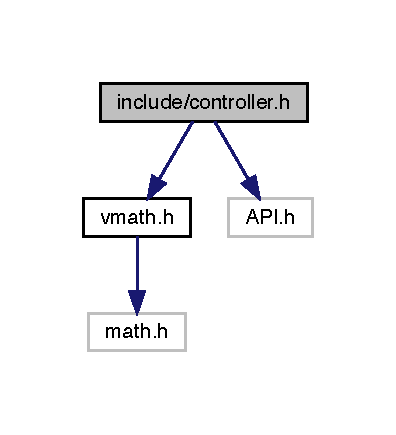
\includegraphics[width=190pt]{controller_8h__incl}
\end{center}
\end{figure}
This graph shows which files directly or indirectly include this file\+:\nopagebreak
\begin{figure}[H]
\begin{center}
\leavevmode
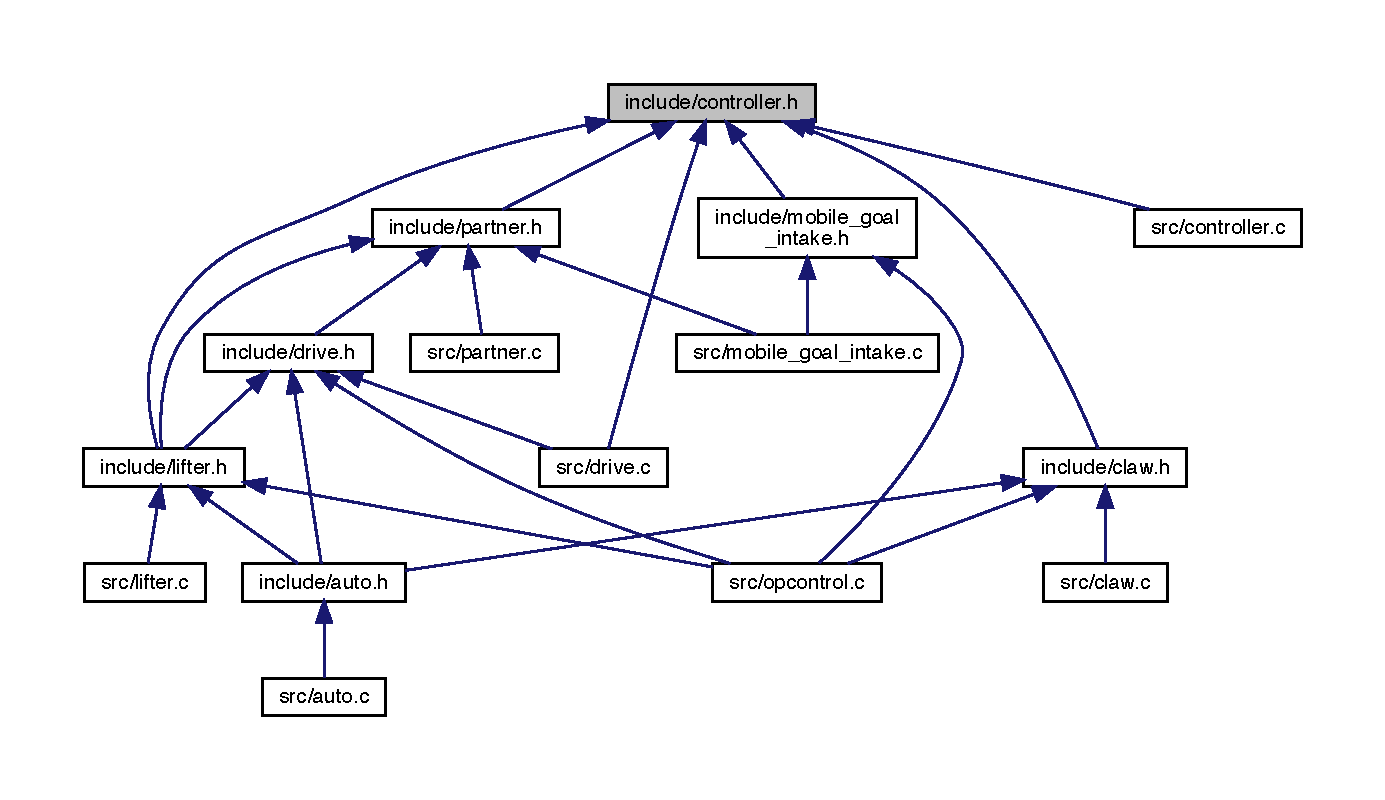
\includegraphics[width=350pt]{controller_8h__dep__incl}
\end{center}
\end{figure}
\subsection*{Macros}
\begin{DoxyCompactItemize}
\item 
\#define \textbf{ L\+E\+F\+T\+\_\+\+B\+U\+M\+P\+E\+RS}~6
\item 
\#define \textbf{ L\+E\+F\+T\+\_\+\+B\+U\+T\+T\+O\+NS}~7
\item 
\#define \textbf{ L\+E\+F\+T\+\_\+\+J\+O\+Y\+\_\+X}~4
\begin{DoxyCompactList}\small\item\em the left x joystick on controller \end{DoxyCompactList}\item 
\#define \textbf{ L\+E\+F\+T\+\_\+\+J\+O\+Y\+\_\+Y}~3
\begin{DoxyCompactList}\small\item\em the left y joystick on controller \end{DoxyCompactList}\item 
\#define \textbf{ M\+A\+S\+T\+ER}~1
\begin{DoxyCompactList}\small\item\em the master controller \end{DoxyCompactList}\item 
\#define \textbf{ P\+A\+R\+T\+N\+ER}~2
\begin{DoxyCompactList}\small\item\em the slave/partner controller \end{DoxyCompactList}\item 
\#define \textbf{ R\+I\+G\+H\+T\+\_\+\+B\+U\+M\+P\+E\+RS}~5
\item 
\#define \textbf{ R\+I\+G\+H\+T\+\_\+\+B\+U\+T\+T\+O\+NS}~8
\item 
\#define \textbf{ R\+I\+G\+H\+T\+\_\+\+J\+O\+Y\+\_\+X}~1
\begin{DoxyCompactList}\small\item\em the right x joystick on controller \end{DoxyCompactList}\item 
\#define \textbf{ R\+I\+G\+H\+T\+\_\+\+J\+O\+Y\+\_\+Y}~2
\begin{DoxyCompactList}\small\item\em the right y joystick on controller \end{DoxyCompactList}\end{DoxyCompactItemize}
\subsection*{Enumerations}
\begin{DoxyCompactItemize}
\item 
enum \textbf{ joystick} \{ \textbf{ R\+I\+G\+H\+T\+\_\+\+J\+OY}, 
\textbf{ L\+E\+F\+T\+\_\+\+J\+OY}
 \}\begin{DoxyCompactList}\small\item\em Represents a joystick on the controller. \end{DoxyCompactList}
\end{DoxyCompactItemize}
\subsection*{Functions}
\begin{DoxyCompactItemize}
\item 
struct \textbf{ cord} \textbf{ get\+\_\+joystick\+\_\+cord} (enum \textbf{ joystick} \textbf{ side}, int controller)
\begin{DoxyCompactList}\small\item\em Gets the location of a joystick on the controller. \end{DoxyCompactList}\end{DoxyCompactItemize}


\subsection{Detailed Description}
controller definitions, macros and functions to assist with usig the vex controllers. 

\begin{DoxyAuthor}{Author}
Chris Jerrett, Christian Desimone 
\end{DoxyAuthor}
\begin{DoxyDate}{Date}
9/9/2017 
\end{DoxyDate}


Definition in file \textbf{ controller.\+h}.



\subsection{Macro Definition Documentation}
\mbox{\label{controller_8h_ad61eb6d28a76985afb8d39ef925541bb}} 
\index{controller.\+h@{controller.\+h}!L\+E\+F\+T\+\_\+\+B\+U\+M\+P\+E\+RS@{L\+E\+F\+T\+\_\+\+B\+U\+M\+P\+E\+RS}}
\index{L\+E\+F\+T\+\_\+\+B\+U\+M\+P\+E\+RS@{L\+E\+F\+T\+\_\+\+B\+U\+M\+P\+E\+RS}!controller.\+h@{controller.\+h}}
\subsubsection{L\+E\+F\+T\+\_\+\+B\+U\+M\+P\+E\+RS}
{\footnotesize\ttfamily \#define L\+E\+F\+T\+\_\+\+B\+U\+M\+P\+E\+RS~6}



Definition at line \textbf{ 18} of file \textbf{ controller.\+h}.

\mbox{\label{controller_8h_a9b885de9f143efd0c862ceb054256536}} 
\index{controller.\+h@{controller.\+h}!L\+E\+F\+T\+\_\+\+B\+U\+T\+T\+O\+NS@{L\+E\+F\+T\+\_\+\+B\+U\+T\+T\+O\+NS}}
\index{L\+E\+F\+T\+\_\+\+B\+U\+T\+T\+O\+NS@{L\+E\+F\+T\+\_\+\+B\+U\+T\+T\+O\+NS}!controller.\+h@{controller.\+h}}
\subsubsection{L\+E\+F\+T\+\_\+\+B\+U\+T\+T\+O\+NS}
{\footnotesize\ttfamily \#define L\+E\+F\+T\+\_\+\+B\+U\+T\+T\+O\+NS~7}



Definition at line \textbf{ 16} of file \textbf{ controller.\+h}.

\mbox{\label{controller_8h_ac055a23829dc64aa20b8e2e1bcfbf316}} 
\index{controller.\+h@{controller.\+h}!L\+E\+F\+T\+\_\+\+J\+O\+Y\+\_\+X@{L\+E\+F\+T\+\_\+\+J\+O\+Y\+\_\+X}}
\index{L\+E\+F\+T\+\_\+\+J\+O\+Y\+\_\+X@{L\+E\+F\+T\+\_\+\+J\+O\+Y\+\_\+X}!controller.\+h@{controller.\+h}}
\subsubsection{L\+E\+F\+T\+\_\+\+J\+O\+Y\+\_\+X}
{\footnotesize\ttfamily \#define L\+E\+F\+T\+\_\+\+J\+O\+Y\+\_\+X~4}



the left x joystick on controller 

\begin{DoxyDate}{Date}
9/1/2017 
\end{DoxyDate}
\begin{DoxyAuthor}{Author}
Chris Jerrett 
\end{DoxyAuthor}


Definition at line \textbf{ 53} of file \textbf{ controller.\+h}.



Referenced by \textbf{ get\+\_\+joystick\+\_\+cord()}.

\mbox{\label{controller_8h_ae0a2b64db5fc4f4bf4b169185be93db3}} 
\index{controller.\+h@{controller.\+h}!L\+E\+F\+T\+\_\+\+J\+O\+Y\+\_\+Y@{L\+E\+F\+T\+\_\+\+J\+O\+Y\+\_\+Y}}
\index{L\+E\+F\+T\+\_\+\+J\+O\+Y\+\_\+Y@{L\+E\+F\+T\+\_\+\+J\+O\+Y\+\_\+Y}!controller.\+h@{controller.\+h}}
\subsubsection{L\+E\+F\+T\+\_\+\+J\+O\+Y\+\_\+Y}
{\footnotesize\ttfamily \#define L\+E\+F\+T\+\_\+\+J\+O\+Y\+\_\+Y~3}



the left y joystick on controller 

\begin{DoxyDate}{Date}
9/1/2017 
\end{DoxyDate}
\begin{DoxyAuthor}{Author}
Chris Jerrett 
\end{DoxyAuthor}


Definition at line \textbf{ 60} of file \textbf{ controller.\+h}.



Referenced by \textbf{ get\+\_\+joystick\+\_\+cord()}.

\mbox{\label{controller_8h_a3fa2d3bf1901157f734a584d47b25d8b}} 
\index{controller.\+h@{controller.\+h}!M\+A\+S\+T\+ER@{M\+A\+S\+T\+ER}}
\index{M\+A\+S\+T\+ER@{M\+A\+S\+T\+ER}!controller.\+h@{controller.\+h}}
\subsubsection{M\+A\+S\+T\+ER}
{\footnotesize\ttfamily \#define M\+A\+S\+T\+ER~1}



the master controller 

\begin{DoxyDate}{Date}
9/1/2017 
\end{DoxyDate}
\begin{DoxyAuthor}{Author}
Chris Jerrett 
\end{DoxyAuthor}


Definition at line \textbf{ 25} of file \textbf{ controller.\+h}.



Referenced by \textbf{ update\+\_\+drive\+\_\+motors()}, and \textbf{ update\+Intake()}.

\mbox{\label{controller_8h_a136e64cf351535da81cacb6a546cade6}} 
\index{controller.\+h@{controller.\+h}!P\+A\+R\+T\+N\+ER@{P\+A\+R\+T\+N\+ER}}
\index{P\+A\+R\+T\+N\+ER@{P\+A\+R\+T\+N\+ER}!controller.\+h@{controller.\+h}}
\subsubsection{P\+A\+R\+T\+N\+ER}
{\footnotesize\ttfamily \#define P\+A\+R\+T\+N\+ER~2}



the slave/partner controller 

\begin{DoxyDate}{Date}
9/1/2017 
\end{DoxyDate}
\begin{DoxyAuthor}{Author}
Chris Jerrett 
\end{DoxyAuthor}


Definition at line \textbf{ 32} of file \textbf{ controller.\+h}.



Referenced by \textbf{ update\+\_\+control()}, \textbf{ update\+\_\+drive\+\_\+motors()}, and \textbf{ update\+Intake()}.

\mbox{\label{controller_8h_a635896b08789914290171051d1b82465}} 
\index{controller.\+h@{controller.\+h}!R\+I\+G\+H\+T\+\_\+\+B\+U\+M\+P\+E\+RS@{R\+I\+G\+H\+T\+\_\+\+B\+U\+M\+P\+E\+RS}}
\index{R\+I\+G\+H\+T\+\_\+\+B\+U\+M\+P\+E\+RS@{R\+I\+G\+H\+T\+\_\+\+B\+U\+M\+P\+E\+RS}!controller.\+h@{controller.\+h}}
\subsubsection{R\+I\+G\+H\+T\+\_\+\+B\+U\+M\+P\+E\+RS}
{\footnotesize\ttfamily \#define R\+I\+G\+H\+T\+\_\+\+B\+U\+M\+P\+E\+RS~5}



Definition at line \textbf{ 17} of file \textbf{ controller.\+h}.

\mbox{\label{controller_8h_a68881b6085c880930037b20764fe5aee}} 
\index{controller.\+h@{controller.\+h}!R\+I\+G\+H\+T\+\_\+\+B\+U\+T\+T\+O\+NS@{R\+I\+G\+H\+T\+\_\+\+B\+U\+T\+T\+O\+NS}}
\index{R\+I\+G\+H\+T\+\_\+\+B\+U\+T\+T\+O\+NS@{R\+I\+G\+H\+T\+\_\+\+B\+U\+T\+T\+O\+NS}!controller.\+h@{controller.\+h}}
\subsubsection{R\+I\+G\+H\+T\+\_\+\+B\+U\+T\+T\+O\+NS}
{\footnotesize\ttfamily \#define R\+I\+G\+H\+T\+\_\+\+B\+U\+T\+T\+O\+NS~8}



Definition at line \textbf{ 15} of file \textbf{ controller.\+h}.

\mbox{\label{controller_8h_ad74f84aad465437cc1e0f914dbd6fab5}} 
\index{controller.\+h@{controller.\+h}!R\+I\+G\+H\+T\+\_\+\+J\+O\+Y\+\_\+X@{R\+I\+G\+H\+T\+\_\+\+J\+O\+Y\+\_\+X}}
\index{R\+I\+G\+H\+T\+\_\+\+J\+O\+Y\+\_\+X@{R\+I\+G\+H\+T\+\_\+\+J\+O\+Y\+\_\+X}!controller.\+h@{controller.\+h}}
\subsubsection{R\+I\+G\+H\+T\+\_\+\+J\+O\+Y\+\_\+X}
{\footnotesize\ttfamily \#define R\+I\+G\+H\+T\+\_\+\+J\+O\+Y\+\_\+X~1}



the right x joystick on controller 

\begin{DoxyDate}{Date}
9/1/2017 
\end{DoxyDate}
\begin{DoxyAuthor}{Author}
Chris Jerrett 
\end{DoxyAuthor}


Definition at line \textbf{ 39} of file \textbf{ controller.\+h}.



Referenced by \textbf{ get\+\_\+joystick\+\_\+cord()}.

\mbox{\label{controller_8h_a99457bf9dee795334411ea77f0858b16}} 
\index{controller.\+h@{controller.\+h}!R\+I\+G\+H\+T\+\_\+\+J\+O\+Y\+\_\+Y@{R\+I\+G\+H\+T\+\_\+\+J\+O\+Y\+\_\+Y}}
\index{R\+I\+G\+H\+T\+\_\+\+J\+O\+Y\+\_\+Y@{R\+I\+G\+H\+T\+\_\+\+J\+O\+Y\+\_\+Y}!controller.\+h@{controller.\+h}}
\subsubsection{R\+I\+G\+H\+T\+\_\+\+J\+O\+Y\+\_\+Y}
{\footnotesize\ttfamily \#define R\+I\+G\+H\+T\+\_\+\+J\+O\+Y\+\_\+Y~2}



the right y joystick on controller 

\begin{DoxyDate}{Date}
9/1/2017 
\end{DoxyDate}
\begin{DoxyAuthor}{Author}
Chris Jerrett 
\end{DoxyAuthor}


Definition at line \textbf{ 46} of file \textbf{ controller.\+h}.



Referenced by \textbf{ get\+\_\+joystick\+\_\+cord()}.



\subsection{Enumeration Type Documentation}
\mbox{\label{controller_8h_ac365c9e892abe4a1b85ae8f56a4eae5a}} 
\index{controller.\+h@{controller.\+h}!joystick@{joystick}}
\index{joystick@{joystick}!controller.\+h@{controller.\+h}}
\subsubsection{joystick}
{\footnotesize\ttfamily enum \textbf{ joystick}}



Represents a joystick on the controller. 

\begin{DoxyDate}{Date}
9/10/2017 
\end{DoxyDate}
\begin{DoxyAuthor}{Author}
Chris Jerrett 
\end{DoxyAuthor}
\begin{DoxyEnumFields}{Enumerator}
\raisebox{\heightof{T}}[0pt][0pt]{\index{R\+I\+G\+H\+T\+\_\+\+J\+OY@{R\+I\+G\+H\+T\+\_\+\+J\+OY}!controller.\+h@{controller.\+h}}\index{controller.\+h@{controller.\+h}!R\+I\+G\+H\+T\+\_\+\+J\+OY@{R\+I\+G\+H\+T\+\_\+\+J\+OY}}}\mbox{\label{controller_8h_ac365c9e892abe4a1b85ae8f56a4eae5aae08a2d362c677f96f72d93047513cafe}} 
R\+I\+G\+H\+T\+\_\+\+J\+OY&The right joystick \\
\hline

\raisebox{\heightof{T}}[0pt][0pt]{\index{L\+E\+F\+T\+\_\+\+J\+OY@{L\+E\+F\+T\+\_\+\+J\+OY}!controller.\+h@{controller.\+h}}\index{controller.\+h@{controller.\+h}!L\+E\+F\+T\+\_\+\+J\+OY@{L\+E\+F\+T\+\_\+\+J\+OY}}}\mbox{\label{controller_8h_ac365c9e892abe4a1b85ae8f56a4eae5aaf822d7888862e67a3c624775b85c50a9}} 
L\+E\+F\+T\+\_\+\+J\+OY&The left joystick \\
\hline

\end{DoxyEnumFields}


Definition at line \textbf{ 67} of file \textbf{ controller.\+h}.


\begin{DoxyCode}
00067               \{
00069   RIGHT_JOY,
00071   LEFT_JOY,
00072 \};
\end{DoxyCode}


\subsection{Function Documentation}
\mbox{\label{controller_8h_a0ce0176099c0bb15ad8c36123222059d}} 
\index{controller.\+h@{controller.\+h}!get\+\_\+joystick\+\_\+cord@{get\+\_\+joystick\+\_\+cord}}
\index{get\+\_\+joystick\+\_\+cord@{get\+\_\+joystick\+\_\+cord}!controller.\+h@{controller.\+h}}
\subsubsection{get\+\_\+joystick\+\_\+cord()}
{\footnotesize\ttfamily struct \textbf{ cord} get\+\_\+joystick\+\_\+cord (\begin{DoxyParamCaption}\item[{enum \textbf{ joystick}}]{side,  }\item[{int}]{controller }\end{DoxyParamCaption})}



Gets the location of a joystick on the controller. 

\begin{DoxyAuthor}{Author}
Chris Jerrett 
\end{DoxyAuthor}


Definition at line \textbf{ 7} of file \textbf{ controller.\+c}.



References \textbf{ L\+E\+F\+T\+\_\+\+J\+O\+Y\+\_\+X}, \textbf{ L\+E\+F\+T\+\_\+\+J\+O\+Y\+\_\+Y}, \textbf{ R\+I\+G\+H\+T\+\_\+\+J\+OY}, \textbf{ R\+I\+G\+H\+T\+\_\+\+J\+O\+Y\+\_\+X}, \textbf{ R\+I\+G\+H\+T\+\_\+\+J\+O\+Y\+\_\+Y}, \textbf{ cord\+::x}, and \textbf{ cord\+::y}.


\begin{DoxyCode}
00007                                                                   \{
00008   \textcolor{keywordtype}{int} x;
00009   \textcolor{keywordtype}{int} y;
00010   \textcolor{comment}{//Get the joystick value for either the right or left,}
00011   \textcolor{comment}{//depending on the mode}
00012   \textcolor{keywordflow}{if}(side == RIGHT_JOY) \{
00013     y = joystickGetAnalog(controller, RIGHT_JOY_X);
00014     x = joystickGetAnalog(controller, RIGHT_JOY_Y);
00015   \} \textcolor{keywordflow}{else} \{
00016     y = joystickGetAnalog(controller, LEFT_JOY_X);
00017     x = joystickGetAnalog(controller, LEFT_JOY_Y);
00018   \}
00019   \textcolor{comment}{//Define a coordinate for the joystick value}
00020   \textcolor{keyword}{struct }cord c;
00021   c.x = x;
00022   c.y = y;
00023   \textcolor{keywordflow}{return} c;
00024 \}
\end{DoxyCode}

\subsection{include/drive.h File Reference}
\label{drive_8h}\index{include/drive.\+h@{include/drive.\+h}}


Drive base definitions and enumerations.  


{\ttfamily \#include $<$A\+P\+I.\+h$>$}\newline
{\ttfamily \#include \char`\"{}partner.\+h\char`\"{}}\newline
Include dependency graph for drive.\+h\+:\nopagebreak
\begin{figure}[H]
\begin{center}
\leavevmode
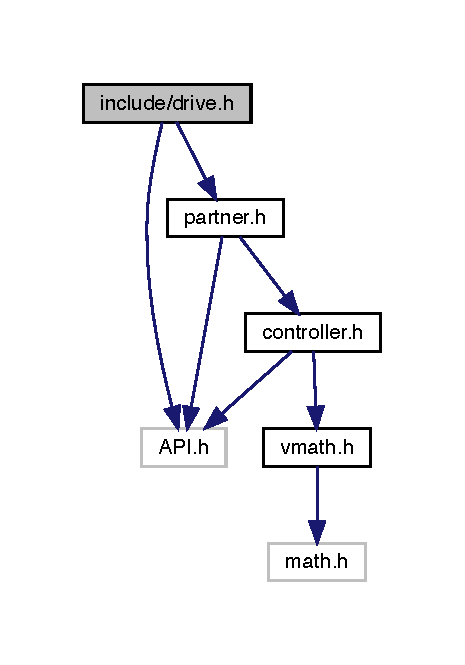
\includegraphics[width=350pt]{drive_8h__incl}
\end{center}
\end{figure}
This graph shows which files directly or indirectly include this file\+:\nopagebreak
\begin{figure}[H]
\begin{center}
\leavevmode
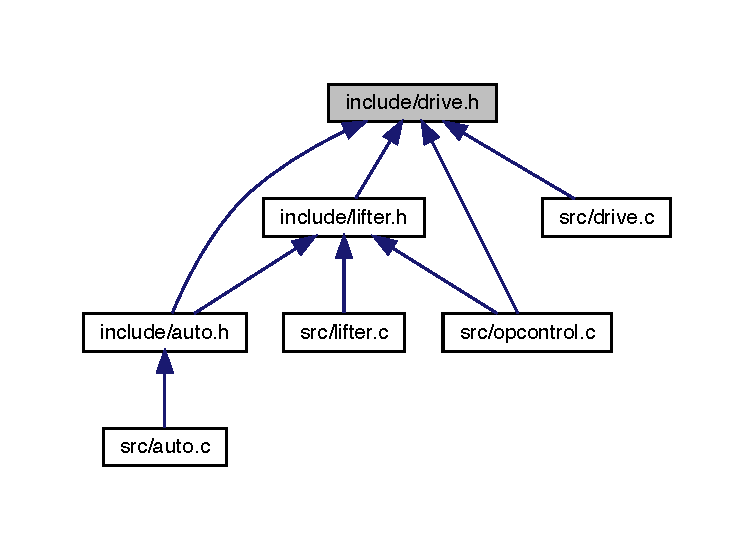
\includegraphics[width=350pt]{drive_8h__dep__incl}
\end{center}
\end{figure}
\subsubsection*{Macros}
\begin{DoxyCompactItemize}
\item 
\#define \textbf{ T\+H\+R\+E\+S\+H\+O\+LD}~10
\begin{DoxyCompactList}\small\item\em The dead spot on the controller to avoid running motors at low speeds. \end{DoxyCompactList}\end{DoxyCompactItemize}
\subsubsection*{Typedefs}
\begin{DoxyCompactItemize}
\item 
typedef enum \textbf{ side} \textbf{ side\+\_\+t}
\begin{DoxyCompactList}\small\item\em enumeration indication side of the robot. \end{DoxyCompactList}\end{DoxyCompactItemize}
\subsubsection*{Enumerations}
\begin{DoxyCompactItemize}
\item 
enum \textbf{ side} \{ \textbf{ L\+E\+FT}, 
\textbf{ B\+O\+TH}, 
\textbf{ R\+I\+G\+HT}
 \}\begin{DoxyCompactList}\small\item\em enumeration indication side of the robot. \end{DoxyCompactList}
\end{DoxyCompactItemize}
\subsubsection*{Functions}
\begin{DoxyCompactItemize}
\item 
void \textbf{ set\+\_\+side\+\_\+speed} (\textbf{ side\+\_\+t} \textbf{ side}, int speed)
\begin{DoxyCompactList}\small\item\em sets the speed of one side of the robot. \end{DoxyCompactList}\item 
void \textbf{ set\+Thresh} (int t)
\begin{DoxyCompactList}\small\item\em Sets the deadzone threshhold on the drive. \end{DoxyCompactList}\item 
void \textbf{ update\+\_\+drive\+\_\+motors} ()
\begin{DoxyCompactList}\small\item\em Updates the drive motors during teleop. \end{DoxyCompactList}\end{DoxyCompactItemize}


\subsubsection{Detailed Description}
Drive base definitions and enumerations. 

\begin{DoxyAuthor}{Author}
Chris Jerrett 
\end{DoxyAuthor}
\begin{DoxyDate}{Date}
9/9/2017 
\end{DoxyDate}


Definition in file \textbf{ drive.\+h}.



\subsubsection{Macro Definition Documentation}
\mbox{\label{drive_8h_a4679d8ea8690999a6c6c7c0cb245c879}} 
\index{drive.\+h@{drive.\+h}!T\+H\+R\+E\+S\+H\+O\+LD@{T\+H\+R\+E\+S\+H\+O\+LD}}
\index{T\+H\+R\+E\+S\+H\+O\+LD@{T\+H\+R\+E\+S\+H\+O\+LD}!drive.\+h@{drive.\+h}}
\paragraph{T\+H\+R\+E\+S\+H\+O\+LD}
{\footnotesize\ttfamily \#define T\+H\+R\+E\+S\+H\+O\+LD~10}



The dead spot on the controller to avoid running motors at low speeds. 



Definition at line \textbf{ 18} of file \textbf{ drive.\+h}.



Referenced by \textbf{ joystick\+Exp()}, and \textbf{ update\+\_\+lifter()}.



\subsubsection{Typedef Documentation}
\mbox{\label{drive_8h_a9df2afd2f1acb97019655e5e730609c7}} 
\index{drive.\+h@{drive.\+h}!side\+\_\+t@{side\+\_\+t}}
\index{side\+\_\+t@{side\+\_\+t}!drive.\+h@{drive.\+h}}
\paragraph{side\+\_\+t}
{\footnotesize\ttfamily typedef enum \textbf{ side}  \textbf{ side\+\_\+t}}



enumeration indication side of the robot. 

\begin{DoxyAuthor}{Author}
Christian Desimone 
\end{DoxyAuthor}
\begin{DoxyDate}{Date}
9/7/2017 Side can be right, both of left. Contained in side typedef, so enum is unnecessary. 
\end{DoxyDate}


\subsubsection{Enumeration Type Documentation}
\mbox{\label{drive_8h_afc015eff6557e84151d2e53b94375445}} 
\index{drive.\+h@{drive.\+h}!side@{side}}
\index{side@{side}!drive.\+h@{drive.\+h}}
\paragraph{side}
{\footnotesize\ttfamily enum \textbf{ side}}



enumeration indication side of the robot. 

\begin{DoxyAuthor}{Author}
Christian Desimone 
\end{DoxyAuthor}
\begin{DoxyDate}{Date}
9/7/2017 Side can be right, both of left. Contained in side typedef, so enum is unnecessary. 
\end{DoxyDate}
\begin{DoxyEnumFields}{Enumerator}
\raisebox{\heightof{T}}[0pt][0pt]{\index{L\+E\+FT@{L\+E\+FT}!drive.\+h@{drive.\+h}}\index{drive.\+h@{drive.\+h}!L\+E\+FT@{L\+E\+FT}}}\mbox{\label{drive_8h_afc015eff6557e84151d2e53b94375445adb45120aafd37a973140edee24708065}} 
L\+E\+FT&\\
\hline

\raisebox{\heightof{T}}[0pt][0pt]{\index{B\+O\+TH@{B\+O\+TH}!drive.\+h@{drive.\+h}}\index{drive.\+h@{drive.\+h}!B\+O\+TH@{B\+O\+TH}}}\mbox{\label{drive_8h_afc015eff6557e84151d2e53b94375445a627abe5a430420baf29ebe1940a7f2fb}} 
B\+O\+TH&\\
\hline

\raisebox{\heightof{T}}[0pt][0pt]{\index{R\+I\+G\+HT@{R\+I\+G\+HT}!drive.\+h@{drive.\+h}}\index{drive.\+h@{drive.\+h}!R\+I\+G\+HT@{R\+I\+G\+HT}}}\mbox{\label{drive_8h_afc015eff6557e84151d2e53b94375445aec8379af7490bb9eaaf579cf17876f38}} 
R\+I\+G\+HT&\\
\hline

\end{DoxyEnumFields}


Definition at line \textbf{ 26} of file \textbf{ drive.\+h}.


\begin{DoxyCode}
00026                  \{
00027   LEFT,
00028   BOTH,
00029   RIGHT
00030 \} side_t;
\end{DoxyCode}


\subsubsection{Function Documentation}
\mbox{\label{drive_8h_a8df41fd50094c065eedc81fc5e6595d1}} 
\index{drive.\+h@{drive.\+h}!set\+\_\+side\+\_\+speed@{set\+\_\+side\+\_\+speed}}
\index{set\+\_\+side\+\_\+speed@{set\+\_\+side\+\_\+speed}!drive.\+h@{drive.\+h}}
\paragraph{set\+\_\+side\+\_\+speed()}
{\footnotesize\ttfamily void set\+\_\+side\+\_\+speed (\begin{DoxyParamCaption}\item[{\textbf{ side\+\_\+t}}]{side,  }\item[{int}]{speed }\end{DoxyParamCaption})}



sets the speed of one side of the robot. 

\begin{DoxyAuthor}{Author}
Christian Desimone 
\end{DoxyAuthor}

\begin{DoxyParams}{Parameters}
{\em side} & a side enum which indicates the size. \\
\hline
{\em speed} & the speed of the side. Can range from -\/127 -\/ 127 negative being back and positive forwards \\
\hline
\end{DoxyParams}


Definition at line \textbf{ 68} of file \textbf{ drive.\+c}.



References \textbf{ B\+O\+TH}, \textbf{ L\+E\+FT}, \textbf{ M\+O\+T\+O\+R\+\_\+\+B\+A\+C\+K\+\_\+\+L\+E\+FT}, \textbf{ M\+O\+T\+O\+R\+\_\+\+B\+A\+C\+K\+\_\+\+R\+I\+G\+HT}, \textbf{ M\+O\+T\+O\+R\+\_\+\+F\+R\+O\+N\+T\+\_\+\+L\+E\+FT}, \textbf{ M\+O\+T\+O\+R\+\_\+\+F\+R\+O\+N\+T\+\_\+\+R\+I\+G\+HT}, \textbf{ M\+O\+T\+O\+R\+\_\+\+M\+I\+D\+D\+L\+E\+\_\+\+L\+E\+FT}, \textbf{ M\+O\+T\+O\+R\+\_\+\+M\+I\+D\+D\+L\+E\+\_\+\+R\+I\+G\+HT}, \textbf{ R\+I\+G\+HT}, and \textbf{ set\+\_\+motor\+\_\+slew()}.



Referenced by \textbf{ autonomous()}, and \textbf{ update\+\_\+drive\+\_\+motors()}.


\begin{DoxyCode}
00068                                            \{
00069   \textcolor{keywordflow}{if}(side == RIGHT || side == BOTH)\{
00070     set_motor_slew(MOTOR_BACK_RIGHT , -speed);
00071     set_motor_slew(MOTOR_FRONT_RIGHT, -speed);
00072     set_motor_slew(MOTOR_MIDDLE_RIGHT, -speed);
00073   \}
00074   \textcolor{keywordflow}{if}(side == LEFT || side == BOTH)\{
00075     set_motor_slew(MOTOR_BACK_LEFT, speed);
00076     set_motor_slew(MOTOR_MIDDLE_LEFT, speed);
00077     set_motor_slew(MOTOR_FRONT_LEFT, speed);
00078   \}
00079 \}
\end{DoxyCode}
Here is the call graph for this function\+:\nopagebreak
\begin{figure}[H]
\begin{center}
\leavevmode
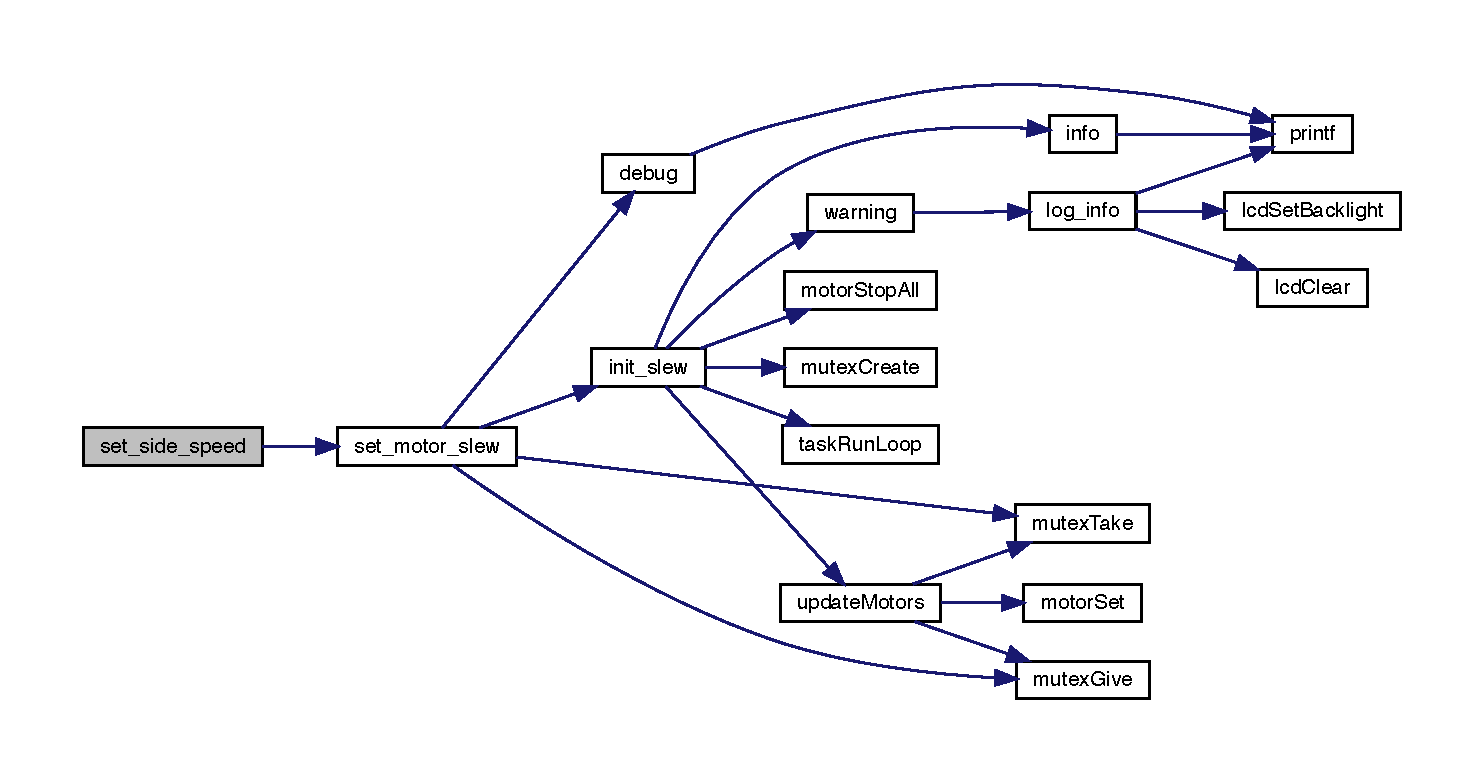
\includegraphics[width=350pt]{drive_8h_a8df41fd50094c065eedc81fc5e6595d1_cgraph}
\end{center}
\end{figure}
Here is the caller graph for this function\+:\nopagebreak
\begin{figure}[H]
\begin{center}
\leavevmode
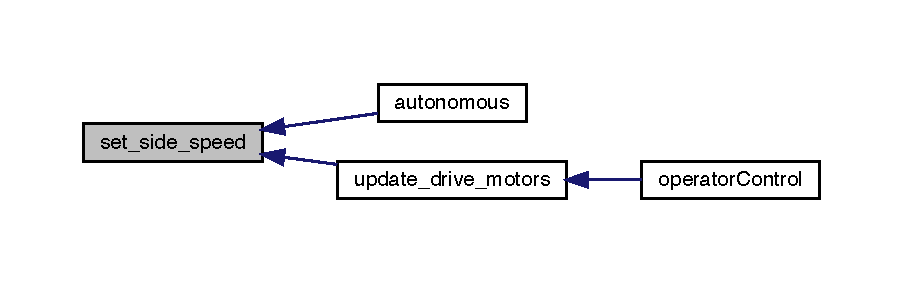
\includegraphics[width=350pt]{drive_8h_a8df41fd50094c065eedc81fc5e6595d1_icgraph}
\end{center}
\end{figure}
\mbox{\label{drive_8h_a53d6e35d53ec3e0b1b1c489d8203f204}} 
\index{drive.\+h@{drive.\+h}!set\+Thresh@{set\+Thresh}}
\index{set\+Thresh@{set\+Thresh}!drive.\+h@{drive.\+h}}
\paragraph{set\+Thresh()}
{\footnotesize\ttfamily void set\+Thresh (\begin{DoxyParamCaption}\item[{int}]{t }\end{DoxyParamCaption})}



Sets the deadzone threshhold on the drive. 

\begin{DoxyAuthor}{Author}
Chris Jerrett

Christian Desimone 
\end{DoxyAuthor}


Definition at line \textbf{ 25} of file \textbf{ drive.\+c}.



References \textbf{ thresh}.


\begin{DoxyCode}
00025                      \{
00026   thresh = t;
00027 \}
\end{DoxyCode}
\mbox{\label{drive_8h_a8224a4626a934d30ed587671b7004bf8}} 
\index{drive.\+h@{drive.\+h}!update\+\_\+drive\+\_\+motors@{update\+\_\+drive\+\_\+motors}}
\index{update\+\_\+drive\+\_\+motors@{update\+\_\+drive\+\_\+motors}!drive.\+h@{drive.\+h}}
\paragraph{update\+\_\+drive\+\_\+motors()}
{\footnotesize\ttfamily void update\+\_\+drive\+\_\+motors (\begin{DoxyParamCaption}{ }\end{DoxyParamCaption})}



Updates the drive motors during teleop. 

\begin{DoxyAuthor}{Author}
Christian Desimone 
\end{DoxyAuthor}
\begin{DoxyDate}{Date}
9/5/17 
\end{DoxyDate}


Definition at line \textbf{ 34} of file \textbf{ drive.\+c}.



References \textbf{ get\+\_\+mode()}, \textbf{ joystick\+Get\+Analog()}, \textbf{ L\+E\+FT}, \textbf{ M\+A\+S\+T\+ER}, \textbf{ P\+A\+R\+T\+N\+ER}, \textbf{ P\+A\+R\+T\+N\+E\+R\+\_\+\+C\+O\+N\+T\+R\+O\+L\+L\+E\+R\+\_\+\+M\+O\+DE}, \textbf{ R\+I\+G\+HT}, \textbf{ set\+\_\+side\+\_\+speed()}, \textbf{ thresh}, \textbf{ cord\+::x}, and \textbf{ cord\+::y}.



Referenced by \textbf{ operator\+Control()}.


\begin{DoxyCode}
00034                           \{
00035   \textcolor{comment}{//Get the joystick values from the controller}
00036   \textcolor{keywordtype}{int} x = 0;
00037   \textcolor{keywordtype}{int} y = 0;
00038   \textcolor{keywordflow}{if}(get_mode() == PARTNER_CONTROLLER_MODE) \{
00039     x = (joystickGetAnalog(PARTNER, 3));
00040     y = (joystickGetAnalog(PARTNER, 1));
00041   \} \textcolor{keywordflow}{else} \{
00042     x = -(joystickGetAnalog(MASTER, 3));
00043     y = (joystickGetAnalog(MASTER, 1));
00044   \}
00045   \textcolor{comment}{//Make sure the joystick values are significant enough to change the motors}
00046   \textcolor{keywordflow}{if}(x < thresh && x > -thresh)\{
00047     x = 0;
00048   \}
00049   \textcolor{keywordflow}{if}(y < thresh && y > -thresh)\{
00050     y = 0;
00051   \}
00052   \textcolor{comment}{//Create motor values for the left and right from the x and y of the joystick}
00053   \textcolor{keywordtype}{int} r = (x + y);
00054   \textcolor{keywordtype}{int} l = -(x - y);
00055 
00056   \textcolor{comment}{//Set the drive motors}
00057   set_side_speed(LEFT, l);
00058   set_side_speed(RIGHT, -r);
00059 
00060 \}
\end{DoxyCode}
Here is the call graph for this function\+:\nopagebreak
\begin{figure}[H]
\begin{center}
\leavevmode
\includegraphics[width=350pt]{drive_8h_a8224a4626a934d30ed587671b7004bf8_cgraph}
\end{center}
\end{figure}
Here is the caller graph for this function\+:\nopagebreak
\begin{figure}[H]
\begin{center}
\leavevmode
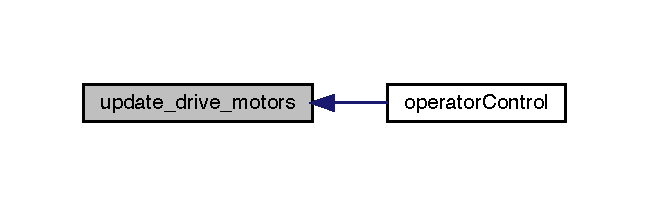
\includegraphics[width=311pt]{drive_8h_a8224a4626a934d30ed587671b7004bf8_icgraph}
\end{center}
\end{figure}

\hypertarget{encoders_8h}{}\section{include/encoders.h File Reference}
\label{encoders_8h}\index{include/encoders.\+h@{include/encoders.\+h}}


wrapper around encoder functions  


{\ttfamily \#include $<$A\+P\+I.\+h$>$}\newline
\subsection*{Macros}
\begin{DoxyCompactItemize}
\item 
\#define \hyperlink{encoders_8h_a87db35d2735ef045f57d446b3bfe8d48}{I\+M\+E\+\_\+\+N\+U\+M\+B\+ER}~0
\begin{DoxyCompactList}\small\item\em The number of I\+M\+Es. This number is compared against the number detect in init\+\_\+encoders. \end{DoxyCompactList}\end{DoxyCompactItemize}
\subsection*{Functions}
\begin{DoxyCompactItemize}
\item 
int \hyperlink{encoders_8h_aed261dd4dae33a48c42f2e363c84760f}{get\+\_\+encoder\+\_\+ticks} (unsigned char address)
\begin{DoxyCompactList}\small\item\em Gets the encoder ticks since last reset. \end{DoxyCompactList}\item 
int \hyperlink{encoders_8h_a8e6b77703c5cf18e00709b052fb4bf22}{get\+\_\+encoder\+\_\+velocity} (unsigned char address)
\begin{DoxyCompactList}\small\item\em Gets the encoder reads. \end{DoxyCompactList}\item 
bool \hyperlink{encoders_8h_aa6ec1ca17e907babd52803ecba451cd3}{init\+\_\+encoders} ()
\begin{DoxyCompactList}\small\item\em Initializes all motor encoders. \end{DoxyCompactList}\end{DoxyCompactItemize}


\subsection{Detailed Description}
wrapper around encoder functions 

\begin{DoxyAuthor}{Author}
Chris Jerrett 
\end{DoxyAuthor}
\begin{DoxyDate}{Date}
9/9/2017 
\end{DoxyDate}


\subsection{Macro Definition Documentation}
\mbox{\Hypertarget{encoders_8h_a87db35d2735ef045f57d446b3bfe8d48}\label{encoders_8h_a87db35d2735ef045f57d446b3bfe8d48}} 
\index{encoders.\+h@{encoders.\+h}!I\+M\+E\+\_\+\+N\+U\+M\+B\+ER@{I\+M\+E\+\_\+\+N\+U\+M\+B\+ER}}
\index{I\+M\+E\+\_\+\+N\+U\+M\+B\+ER@{I\+M\+E\+\_\+\+N\+U\+M\+B\+ER}!encoders.\+h@{encoders.\+h}}
\subsubsection{\texorpdfstring{I\+M\+E\+\_\+\+N\+U\+M\+B\+ER}{IME\_NUMBER}}
{\footnotesize\ttfamily \#define I\+M\+E\+\_\+\+N\+U\+M\+B\+ER~0}



The number of I\+M\+Es. This number is compared against the number detect in init\+\_\+encoders. 

\begin{DoxySeeAlso}{See also}
\hyperlink{encoders_8h_aa6ec1ca17e907babd52803ecba451cd3}{init\+\_\+encoders()} 
\end{DoxySeeAlso}
\begin{DoxyAuthor}{Author}
Chris Jerrett 
\end{DoxyAuthor}
\begin{DoxyDate}{Date}
9/9/2017 
\end{DoxyDate}
\begin{DoxySeeAlso}{See also}
\hyperlink{encoders_8h_a87db35d2735ef045f57d446b3bfe8d48}{I\+M\+E\+\_\+\+N\+U\+M\+B\+ER} 
\end{DoxySeeAlso}


Definition at line 21 of file encoders.\+h.



Referenced by init\+\_\+encoders().



\subsection{Function Documentation}
\mbox{\Hypertarget{encoders_8h_aed261dd4dae33a48c42f2e363c84760f}\label{encoders_8h_aed261dd4dae33a48c42f2e363c84760f}} 
\index{encoders.\+h@{encoders.\+h}!get\+\_\+encoder\+\_\+ticks@{get\+\_\+encoder\+\_\+ticks}}
\index{get\+\_\+encoder\+\_\+ticks@{get\+\_\+encoder\+\_\+ticks}!encoders.\+h@{encoders.\+h}}
\subsubsection{\texorpdfstring{get\+\_\+encoder\+\_\+ticks()}{get\_encoder\_ticks()}}
{\footnotesize\ttfamily int get\+\_\+encoder\+\_\+ticks (\begin{DoxyParamCaption}\item[{unsigned char}]{address }\end{DoxyParamCaption})}



Gets the encoder ticks since last reset. 

\begin{DoxyAuthor}{Author}
Chris Jerrett 
\end{DoxyAuthor}
\begin{DoxyDate}{Date}
9/15/2017 
\end{DoxyDate}


Definition at line 12 of file encoders.\+c.


\begin{DoxyCode}
12                                              \{
13   \textcolor{keywordtype}{int} i = 0;
14   imeGet(address, &i);
15   \textcolor{keywordflow}{return} i;
16 \}
\end{DoxyCode}
\mbox{\Hypertarget{encoders_8h_a8e6b77703c5cf18e00709b052fb4bf22}\label{encoders_8h_a8e6b77703c5cf18e00709b052fb4bf22}} 
\index{encoders.\+h@{encoders.\+h}!get\+\_\+encoder\+\_\+velocity@{get\+\_\+encoder\+\_\+velocity}}
\index{get\+\_\+encoder\+\_\+velocity@{get\+\_\+encoder\+\_\+velocity}!encoders.\+h@{encoders.\+h}}
\subsubsection{\texorpdfstring{get\+\_\+encoder\+\_\+velocity()}{get\_encoder\_velocity()}}
{\footnotesize\ttfamily int get\+\_\+encoder\+\_\+velocity (\begin{DoxyParamCaption}\item[{unsigned char}]{address }\end{DoxyParamCaption})}



Gets the encoder reads. 

\begin{DoxyAuthor}{Author}
Chris Jerrett 
\end{DoxyAuthor}
\begin{DoxyDate}{Date}
9/15/2017 
\end{DoxyDate}


Definition at line 18 of file encoders.\+c.


\begin{DoxyCode}
18                                                 \{
19   \textcolor{keywordtype}{int} i = 0;
20   imeGetVelocity(address, &i);
21   \textcolor{keywordflow}{return} i;
22 \}
\end{DoxyCode}
\mbox{\Hypertarget{encoders_8h_aa6ec1ca17e907babd52803ecba451cd3}\label{encoders_8h_aa6ec1ca17e907babd52803ecba451cd3}} 
\index{encoders.\+h@{encoders.\+h}!init\+\_\+encoders@{init\+\_\+encoders}}
\index{init\+\_\+encoders@{init\+\_\+encoders}!encoders.\+h@{encoders.\+h}}
\subsubsection{\texorpdfstring{init\+\_\+encoders()}{init\_encoders()}}
{\footnotesize\ttfamily bool init\+\_\+encoders (\begin{DoxyParamCaption}{ }\end{DoxyParamCaption})}



Initializes all motor encoders. 

\begin{DoxyAuthor}{Author}
Chris Jerrett 
\end{DoxyAuthor}
\begin{DoxyDate}{Date}
9/9/2017 
\end{DoxyDate}
\begin{DoxySeeAlso}{See also}
\hyperlink{encoders_8h_a87db35d2735ef045f57d446b3bfe8d48}{I\+M\+E\+\_\+\+N\+U\+M\+B\+ER} 
\end{DoxySeeAlso}


Definition at line 4 of file encoders.\+c.



References I\+M\+E\+\_\+\+N\+U\+M\+B\+ER.



Referenced by initialize().


\begin{DoxyCode}
4                      \{
5 \textcolor{preprocessor}{  #ifdef IME\_NUMBER}
6   \textcolor{keywordflow}{return} imeInitializeAll() == \hyperlink{encoders_8h_a87db35d2735ef045f57d446b3bfe8d48}{IME\_NUMBER};
7 \textcolor{preprocessor}{  #else}
8   \textcolor{keywordflow}{return} imeInitializeAll();
9 \textcolor{preprocessor}{  #endif}
10 \}
\end{DoxyCode}

\subsection{include/lcd.h File Reference}
\label{lcd_8h}\index{include/lcd.\+h@{include/lcd.\+h}}


L\+CD wrapper functions and macros.  


{\ttfamily \#include $<$A\+P\+I.\+h$>$}\newline
\subsubsection*{Data Structures}
\begin{DoxyCompactItemize}
\item 
struct \textbf{ lcd\+\_\+buttons}
\begin{DoxyCompactList}\small\item\em represents the state of the lcd buttons \end{DoxyCompactList}\end{DoxyCompactItemize}
\subsubsection*{Macros}
\begin{DoxyCompactItemize}
\item 
\#define \textbf{ B\+O\+T\+T\+O\+M\+\_\+\+R\+OW}~2
\begin{DoxyCompactList}\small\item\em The bottom row on the lcd screen. \end{DoxyCompactList}\item 
\#define \textbf{ T\+O\+P\+\_\+\+R\+OW}~1
\begin{DoxyCompactList}\small\item\em The top row on the lcd screen. \end{DoxyCompactList}\end{DoxyCompactItemize}
\subsubsection*{Enumerations}
\begin{DoxyCompactItemize}
\item 
enum \textbf{ button\+\_\+state} \{ \textbf{ R\+E\+L\+E\+A\+S\+ED} = false, 
\textbf{ P\+R\+E\+S\+S\+ED} = true
 \}\begin{DoxyCompactList}\small\item\em Represents the state of a button. \end{DoxyCompactList}
\end{DoxyCompactItemize}
\subsubsection*{Functions}
\begin{DoxyCompactItemize}
\item 
void \textbf{ init\+\_\+main\+\_\+lcd} (F\+I\+LE $\ast$lcd)
\begin{DoxyCompactList}\small\item\em Initializes the lcd screen. Also will initialize the lcd\+\_\+port var. Must be called before any lcd function can be called. \end{DoxyCompactList}\item 
void \textbf{ lcd\+\_\+clear} ()
\begin{DoxyCompactList}\small\item\em Clears the lcd. \end{DoxyCompactList}\item 
\textbf{ lcd\+\_\+buttons} \textbf{ lcd\+\_\+get\+\_\+pressed\+\_\+buttons} ()
\begin{DoxyCompactList}\small\item\em Returns the pressed buttons. \end{DoxyCompactList}\item 
void \textbf{ lcd\+\_\+print} (unsigned int line, const char $\ast$str)
\begin{DoxyCompactList}\small\item\em prints a string to a line on the lcd \end{DoxyCompactList}\item 
void \textbf{ lcd\+\_\+printf} (unsigned int line, const char $\ast$format\+\_\+str,...)
\begin{DoxyCompactList}\small\item\em prints a formated string to a line on the lcd. Smilar to printf \end{DoxyCompactList}\item 
void \textbf{ lcd\+\_\+set\+\_\+backlight} (bool \textbf{ state})
\begin{DoxyCompactList}\small\item\em sets the backlight of the lcd \end{DoxyCompactList}\item 
void \textbf{ promt\+\_\+confirmation} (const char $\ast$confirm\+\_\+text)
\begin{DoxyCompactList}\small\item\em Prompts the user to confirm a string. User must press middle button to confirm. Function is not thread safe and will stall a thread. \end{DoxyCompactList}\end{DoxyCompactItemize}


\subsubsection{Detailed Description}
L\+CD wrapper functions and macros. 

\begin{DoxyAuthor}{Author}
Chris Jerrett 
\end{DoxyAuthor}
\begin{DoxyDate}{Date}
9/9/2017 
\end{DoxyDate}


Definition in file \textbf{ lcd.\+h}.



\subsubsection{Macro Definition Documentation}
\mbox{\label{lcd_8h_a7b55e87550874687b3e25a64e1cfda9d}} 
\index{lcd.\+h@{lcd.\+h}!B\+O\+T\+T\+O\+M\+\_\+\+R\+OW@{B\+O\+T\+T\+O\+M\+\_\+\+R\+OW}}
\index{B\+O\+T\+T\+O\+M\+\_\+\+R\+OW@{B\+O\+T\+T\+O\+M\+\_\+\+R\+OW}!lcd.\+h@{lcd.\+h}}
\paragraph{B\+O\+T\+T\+O\+M\+\_\+\+R\+OW}
{\footnotesize\ttfamily \#define B\+O\+T\+T\+O\+M\+\_\+\+R\+OW~2}



The bottom row on the lcd screen. 

\begin{DoxyAuthor}{Author}
Chris Jerrett 
\end{DoxyAuthor}
\begin{DoxyDate}{Date}
9/9/2017 
\end{DoxyDate}


Definition at line \textbf{ 25} of file \textbf{ lcd.\+h}.



Referenced by \textbf{ log\+\_\+info()}.

\mbox{\label{lcd_8h_a18bab754c6ad16bc35c48333091516c9}} 
\index{lcd.\+h@{lcd.\+h}!T\+O\+P\+\_\+\+R\+OW@{T\+O\+P\+\_\+\+R\+OW}}
\index{T\+O\+P\+\_\+\+R\+OW@{T\+O\+P\+\_\+\+R\+OW}!lcd.\+h@{lcd.\+h}}
\paragraph{T\+O\+P\+\_\+\+R\+OW}
{\footnotesize\ttfamily \#define T\+O\+P\+\_\+\+R\+OW~1}



The top row on the lcd screen. 

\begin{DoxyAuthor}{Author}
Chris Jerrett 
\end{DoxyAuthor}
\begin{DoxyDate}{Date}
9/9/2017 
\end{DoxyDate}


Definition at line \textbf{ 18} of file \textbf{ lcd.\+h}.



Referenced by \textbf{ display\+\_\+menu()}, and \textbf{ log\+\_\+info()}.



\subsubsection{Enumeration Type Documentation}
\mbox{\label{lcd_8h_a0bbab92f5605e16a4162b6c5ccc2c29b}} 
\index{lcd.\+h@{lcd.\+h}!button\+\_\+state@{button\+\_\+state}}
\index{button\+\_\+state@{button\+\_\+state}!lcd.\+h@{lcd.\+h}}
\paragraph{button\+\_\+state}
{\footnotesize\ttfamily enum \textbf{ button\+\_\+state}}



Represents the state of a button. 

A button can be pressed of R\+E\+L\+E\+A\+S\+ED. Release is false which is also 0. P\+R\+E\+S\+S\+ED is true or 1.

\begin{DoxyAuthor}{Author}
Chris Jerrett 
\end{DoxyAuthor}
\begin{DoxyDate}{Date}
9/9/2017 
\end{DoxyDate}
\begin{DoxyEnumFields}{Enumerator}
\raisebox{\heightof{T}}[0pt][0pt]{\index{R\+E\+L\+E\+A\+S\+ED@{R\+E\+L\+E\+A\+S\+ED}!lcd.\+h@{lcd.\+h}}\index{lcd.\+h@{lcd.\+h}!R\+E\+L\+E\+A\+S\+ED@{R\+E\+L\+E\+A\+S\+ED}}}\mbox{\label{lcd_8h_a0bbab92f5605e16a4162b6c5ccc2c29baa38d18fe73a7fc82c112b6917d0b5cd0}} 
R\+E\+L\+E\+A\+S\+ED&A released button \\
\hline

\raisebox{\heightof{T}}[0pt][0pt]{\index{P\+R\+E\+S\+S\+ED@{P\+R\+E\+S\+S\+ED}!lcd.\+h@{lcd.\+h}}\index{lcd.\+h@{lcd.\+h}!P\+R\+E\+S\+S\+ED@{P\+R\+E\+S\+S\+ED}}}\mbox{\label{lcd_8h_a0bbab92f5605e16a4162b6c5ccc2c29ba5ef9a100ac8b4b8d6dec477c377b7901}} 
P\+R\+E\+S\+S\+ED&A pressed button \\
\hline

\end{DoxyEnumFields}


Definition at line \textbf{ 36} of file \textbf{ lcd.\+h}.



\subsubsection{Function Documentation}
\mbox{\label{lcd_8h_a93b26f37d6b1687ad54c90feedfd29ca}} 
\index{lcd.\+h@{lcd.\+h}!init\+\_\+main\+\_\+lcd@{init\+\_\+main\+\_\+lcd}}
\index{init\+\_\+main\+\_\+lcd@{init\+\_\+main\+\_\+lcd}!lcd.\+h@{lcd.\+h}}
\paragraph{init\+\_\+main\+\_\+lcd()}
{\footnotesize\ttfamily void init\+\_\+main\+\_\+lcd (\begin{DoxyParamCaption}\item[{F\+I\+LE $\ast$}]{lcd }\end{DoxyParamCaption})}



Initializes the lcd screen. Also will initialize the lcd\+\_\+port var. Must be called before any lcd function can be called. 


\begin{DoxyParams}{Parameters}
{\em lcd} & the urart port of the lcd screen \\
\hline
\end{DoxyParams}
\begin{DoxySeeAlso}{See also}
uart1 

uart2 
\end{DoxySeeAlso}
\begin{DoxyAuthor}{Author}
Chris Jerrett 
\end{DoxyAuthor}
\begin{DoxyDate}{Date}
9/9/2017 
\end{DoxyDate}


Definition at line \textbf{ 62} of file \textbf{ lcd.\+c}.



References \textbf{ lcd\+\_\+clear()}, and \textbf{ lcd\+\_\+port}.



Referenced by \textbf{ initialize()}.

\mbox{\label{lcd_8h_a35c08b1fa742e650f4873939707b893b}} 
\index{lcd.\+h@{lcd.\+h}!lcd\+\_\+clear@{lcd\+\_\+clear}}
\index{lcd\+\_\+clear@{lcd\+\_\+clear}!lcd.\+h@{lcd.\+h}}
\paragraph{lcd\+\_\+clear()}
{\footnotesize\ttfamily void lcd\+\_\+clear (\begin{DoxyParamCaption}{ }\end{DoxyParamCaption})}



Clears the lcd. 

\begin{DoxyAuthor}{Author}
Chris Jerrett 
\end{DoxyAuthor}
\begin{DoxyDate}{Date}
9/9/2017 
\end{DoxyDate}


Definition at line \textbf{ 47} of file \textbf{ lcd.\+c}.



References \textbf{ lcd\+\_\+assert()}, and \textbf{ lcd\+\_\+port}.



Referenced by \textbf{ display\+\_\+menu()}, and \textbf{ init\+\_\+main\+\_\+lcd()}.

\mbox{\label{lcd_8h_ac7b3225ccc82fcbe067ba9da934f010d}} 
\index{lcd.\+h@{lcd.\+h}!lcd\+\_\+get\+\_\+pressed\+\_\+buttons@{lcd\+\_\+get\+\_\+pressed\+\_\+buttons}}
\index{lcd\+\_\+get\+\_\+pressed\+\_\+buttons@{lcd\+\_\+get\+\_\+pressed\+\_\+buttons}!lcd.\+h@{lcd.\+h}}
\paragraph{lcd\+\_\+get\+\_\+pressed\+\_\+buttons()}
{\footnotesize\ttfamily \textbf{ lcd\+\_\+buttons} lcd\+\_\+get\+\_\+pressed\+\_\+buttons (\begin{DoxyParamCaption}{ }\end{DoxyParamCaption})}



Returns the pressed buttons. 

\begin{DoxyReturn}{Returns}
a struct containing the states of all three buttons. 
\end{DoxyReturn}
\begin{DoxyAuthor}{Author}
Chris Jerrett 
\end{DoxyAuthor}
\begin{DoxyDate}{Date}
9/9/2017 
\end{DoxyDate}
\begin{DoxySeeAlso}{See also}
\doxyref{lcd\+\_\+buttons}{p.}{structlcd__buttons} 
\end{DoxySeeAlso}


Definition at line \textbf{ 28} of file \textbf{ lcd.\+c}.



References \textbf{ lcd\+\_\+assert()}, \textbf{ lcd\+\_\+port}, \textbf{ lcd\+\_\+buttons\+::left}, \textbf{ lcd\+\_\+buttons\+::middle}, \textbf{ P\+R\+E\+S\+S\+ED}, \textbf{ R\+E\+L\+E\+A\+S\+ED}, and \textbf{ lcd\+\_\+buttons\+::right}.



Referenced by \textbf{ display\+\_\+menu()}, and \textbf{ promt\+\_\+confirmation()}.

\mbox{\label{lcd_8h_adabd3f7cdda45119604b488caf22bba8}} 
\index{lcd.\+h@{lcd.\+h}!lcd\+\_\+print@{lcd\+\_\+print}}
\index{lcd\+\_\+print@{lcd\+\_\+print}!lcd.\+h@{lcd.\+h}}
\paragraph{lcd\+\_\+print()}
{\footnotesize\ttfamily void lcd\+\_\+print (\begin{DoxyParamCaption}\item[{unsigned int}]{line,  }\item[{const char $\ast$}]{str }\end{DoxyParamCaption})}



prints a string to a line on the lcd 


\begin{DoxyParams}{Parameters}
{\em line} & the line to print on \\
\hline
{\em str} & string to print \\
\hline
\end{DoxyParams}
\begin{DoxyAuthor}{Author}
Chris Jerrett 
\end{DoxyAuthor}
\begin{DoxyDate}{Date}
9/9/2017 
\end{DoxyDate}


Definition at line \textbf{ 75} of file \textbf{ lcd.\+c}.



References \textbf{ lcd\+\_\+assert()}, and \textbf{ lcd\+\_\+port}.



Referenced by \textbf{ display\+\_\+menu()}, and \textbf{ promt\+\_\+confirmation()}.

\mbox{\label{lcd_8h_aa0d4ca88701dfecf98796e2028482b69}} 
\index{lcd.\+h@{lcd.\+h}!lcd\+\_\+printf@{lcd\+\_\+printf}}
\index{lcd\+\_\+printf@{lcd\+\_\+printf}!lcd.\+h@{lcd.\+h}}
\paragraph{lcd\+\_\+printf()}
{\footnotesize\ttfamily void lcd\+\_\+printf (\begin{DoxyParamCaption}\item[{unsigned int}]{line,  }\item[{const char $\ast$}]{format\+\_\+str,  }\item[{}]{... }\end{DoxyParamCaption})}



prints a formated string to a line on the lcd. Smilar to printf 


\begin{DoxyParams}{Parameters}
{\em line} & the line to print on \\
\hline
{\em format\+\_\+str} & format string string to print \\
\hline
\end{DoxyParams}
\begin{DoxyAuthor}{Author}
Chris Jerrett 
\end{DoxyAuthor}
\begin{DoxyDate}{Date}
9/9/2017 
\end{DoxyDate}


Definition at line \textbf{ 87} of file \textbf{ lcd.\+c}.



References \textbf{ lcd\+\_\+assert()}, and \textbf{ lcd\+\_\+port}.

\mbox{\label{lcd_8h_a245902a4d48a6d9bd1ab308bf9b7e6b5}} 
\index{lcd.\+h@{lcd.\+h}!lcd\+\_\+set\+\_\+backlight@{lcd\+\_\+set\+\_\+backlight}}
\index{lcd\+\_\+set\+\_\+backlight@{lcd\+\_\+set\+\_\+backlight}!lcd.\+h@{lcd.\+h}}
\paragraph{lcd\+\_\+set\+\_\+backlight()}
{\footnotesize\ttfamily void lcd\+\_\+set\+\_\+backlight (\begin{DoxyParamCaption}\item[{bool}]{state }\end{DoxyParamCaption})}



sets the backlight of the lcd 


\begin{DoxyParams}{Parameters}
{\em state} & a boolean representing the state of the backlight. true = on, false = off. \\
\hline
\end{DoxyParams}
\begin{DoxyAuthor}{Author}
Chris Jerrett 
\end{DoxyAuthor}
\begin{DoxyDate}{Date}
9/9/2017 
\end{DoxyDate}


Definition at line \textbf{ 99} of file \textbf{ lcd.\+c}.



References \textbf{ lcd\+\_\+assert()}, and \textbf{ lcd\+\_\+port}.

\mbox{\label{lcd_8h_a99f4683e1990edf624ab216bf327cba4}} 
\index{lcd.\+h@{lcd.\+h}!promt\+\_\+confirmation@{promt\+\_\+confirmation}}
\index{promt\+\_\+confirmation@{promt\+\_\+confirmation}!lcd.\+h@{lcd.\+h}}
\paragraph{promt\+\_\+confirmation()}
{\footnotesize\ttfamily void promt\+\_\+confirmation (\begin{DoxyParamCaption}\item[{const char $\ast$}]{confirm\+\_\+text }\end{DoxyParamCaption})}



Prompts the user to confirm a string. User must press middle button to confirm. Function is not thread safe and will stall a thread. 


\begin{DoxyParams}{Parameters}
{\em confirm\+\_\+text} & the text for the user to confirm. \\
\hline
\end{DoxyParams}
\begin{DoxyAuthor}{Author}
Chris Jerrett 
\end{DoxyAuthor}
\begin{DoxyDate}{Date}
9/9/2017 
\end{DoxyDate}


Definition at line \textbf{ 113} of file \textbf{ lcd.\+c}.



References \textbf{ lcd\+\_\+assert()}, \textbf{ lcd\+\_\+get\+\_\+pressed\+\_\+buttons()}, \textbf{ lcd\+\_\+print()}, and \textbf{ P\+R\+E\+S\+S\+ED}.


\subsection{include/log.h File Reference}
\label{log_8h}\index{include/log.\+h@{include/log.\+h}}


Contains logging functions.  


{\ttfamily \#include \char`\"{}lcd.\+h\char`\"{}}\newline
{\ttfamily \#include $<$A\+P\+I.\+h$>$}\newline
\subsubsection*{Macros}
\begin{DoxyCompactItemize}
\item 
\#define \textbf{ D\+E\+B\+UG}~4
\begin{DoxyCompactList}\small\item\em logging only info debug. most verbose level \end{DoxyCompactList}\item 
\#define \textbf{ E\+R\+R\+OR}~1
\begin{DoxyCompactList}\small\item\em logging only errors. Also displays error to lcd \end{DoxyCompactList}\item 
\#define \textbf{ I\+N\+FO}~3
\begin{DoxyCompactList}\small\item\em logging only info messages and higher. \end{DoxyCompactList}\item 
\#define \textbf{ N\+O\+NE}~0
\begin{DoxyCompactList}\small\item\em No logging. Should be used in competition to reduce serial communication. \end{DoxyCompactList}\item 
\#define \textbf{ W\+A\+R\+N\+I\+NG}~2
\begin{DoxyCompactList}\small\item\em logs errors and warnings. Also displays error to lcd \end{DoxyCompactList}\end{DoxyCompactItemize}
\subsubsection*{Functions}
\begin{DoxyCompactItemize}
\item 
void \textbf{ debug} (const char $\ast$debug\+\_\+message)
\begin{DoxyCompactList}\small\item\em prints a info message \end{DoxyCompactList}\item 
void \textbf{ error} (const char $\ast$error\+\_\+message)
\begin{DoxyCompactList}\small\item\em prints a error message and displays on lcd. Only will print and display if log\+\_\+level is greater than N\+O\+NE \end{DoxyCompactList}\item 
void \textbf{ info} (const char $\ast$info\+\_\+message)
\begin{DoxyCompactList}\small\item\em prints a info message \end{DoxyCompactList}\item 
void \textbf{ init\+\_\+error} (bool use\+\_\+lcd, F\+I\+LE $\ast$lcd)
\begin{DoxyCompactList}\small\item\em Initializes the error lcd system Only required if using lcd. \end{DoxyCompactList}\item 
void \textbf{ warning} (const char $\ast$warning\+\_\+message)
\begin{DoxyCompactList}\small\item\em prints a warning message and displays on lcd. Only will print and display if log\+\_\+level is greater than N\+O\+NE \end{DoxyCompactList}\end{DoxyCompactItemize}


\subsubsection{Detailed Description}
Contains logging functions. 

\begin{DoxyAuthor}{Author}
Chris Jerrett 
\end{DoxyAuthor}
\begin{DoxyDate}{Date}
9/16/2017 
\end{DoxyDate}


Definition in file \textbf{ log.\+h}.



\subsubsection{Macro Definition Documentation}
\mbox{\label{log_8h_ad72dbcf6d0153db1b8d8a58001feed83}} 
\index{log.\+h@{log.\+h}!D\+E\+B\+UG@{D\+E\+B\+UG}}
\index{D\+E\+B\+UG@{D\+E\+B\+UG}!log.\+h@{log.\+h}}
\paragraph{D\+E\+B\+UG}
{\footnotesize\ttfamily \#define D\+E\+B\+UG~4}



logging only info debug. most verbose level 

\begin{DoxyAuthor}{Author}
Chris Jerrett 
\end{DoxyAuthor}
\begin{DoxyDate}{Date}
9/10/17 
\end{DoxyDate}


Definition at line \textbf{ 50} of file \textbf{ log.\+h}.

\mbox{\label{log_8h_a8fe83ac76edc595f6b98cd4a4127aed5}} 
\index{log.\+h@{log.\+h}!E\+R\+R\+OR@{E\+R\+R\+OR}}
\index{E\+R\+R\+OR@{E\+R\+R\+OR}!log.\+h@{log.\+h}}
\paragraph{E\+R\+R\+OR}
{\footnotesize\ttfamily \#define E\+R\+R\+OR~1}



logging only errors. Also displays error to lcd 

\begin{DoxyAuthor}{Author}
Chris Jerrett 
\end{DoxyAuthor}
\begin{DoxyDate}{Date}
9/10/17 
\end{DoxyDate}


Definition at line \textbf{ 27} of file \textbf{ log.\+h}.



Referenced by \textbf{ debug()}, and \textbf{ info()}.

\mbox{\label{log_8h_ae1103fea1e1b3c41ca3322d5389f7162}} 
\index{log.\+h@{log.\+h}!I\+N\+FO@{I\+N\+FO}}
\index{I\+N\+FO@{I\+N\+FO}!log.\+h@{log.\+h}}
\paragraph{I\+N\+FO}
{\footnotesize\ttfamily \#define I\+N\+FO~3}



logging only info messages and higher. 

\begin{DoxyAuthor}{Author}
Chris Jerrett 
\end{DoxyAuthor}
\begin{DoxyDate}{Date}
9/10/17 
\end{DoxyDate}


Definition at line \textbf{ 42} of file \textbf{ log.\+h}.

\mbox{\label{log_8h_a655c84af1b0034986ff56e12e84f983d}} 
\index{log.\+h@{log.\+h}!N\+O\+NE@{N\+O\+NE}}
\index{N\+O\+NE@{N\+O\+NE}!log.\+h@{log.\+h}}
\paragraph{N\+O\+NE}
{\footnotesize\ttfamily \#define N\+O\+NE~0}



No logging. Should be used in competition to reduce serial communication. 

\begin{DoxyAuthor}{Author}
Chris Jerrett 
\end{DoxyAuthor}
\begin{DoxyDate}{Date}
9/10/17 
\end{DoxyDate}


Definition at line \textbf{ 19} of file \textbf{ log.\+h}.



Referenced by \textbf{ error()}.

\mbox{\label{log_8h_a5cb439d9f933fde4cf23caa370c030e7}} 
\index{log.\+h@{log.\+h}!W\+A\+R\+N\+I\+NG@{W\+A\+R\+N\+I\+NG}}
\index{W\+A\+R\+N\+I\+NG@{W\+A\+R\+N\+I\+NG}!log.\+h@{log.\+h}}
\paragraph{W\+A\+R\+N\+I\+NG}
{\footnotesize\ttfamily \#define W\+A\+R\+N\+I\+NG~2}



logs errors and warnings. Also displays error to lcd 

\begin{DoxyAuthor}{Author}
Chris Jerrett 
\end{DoxyAuthor}
\begin{DoxyDate}{Date}
9/10/17 
\end{DoxyDate}


Definition at line \textbf{ 35} of file \textbf{ log.\+h}.



Referenced by \textbf{ warning()}.



\subsubsection{Function Documentation}
\mbox{\label{log_8h_af3668f40d1ad1b4f3418869ac9a31f34}} 
\index{log.\+h@{log.\+h}!debug@{debug}}
\index{debug@{debug}!log.\+h@{log.\+h}}
\paragraph{debug()}
{\footnotesize\ttfamily void debug (\begin{DoxyParamCaption}\item[{const char $\ast$}]{debug\+\_\+message }\end{DoxyParamCaption})}



prints a info message 

Only will print and display if log\+\_\+level is greater than info \begin{DoxySeeAlso}{See also}
\doxyref{log\+\_\+level}{p.}{log_8c_a8cf62743dafa288b58bd7c6028ec28e5} 
\end{DoxySeeAlso}

\begin{DoxyParams}{Parameters}
{\em debug\+\_\+message} & the message \\
\hline
\end{DoxyParams}


Definition at line \textbf{ 77} of file \textbf{ log.\+c}.



References \textbf{ E\+R\+R\+OR}, and \textbf{ log\+\_\+level}.



Referenced by \textbf{ set\+\_\+motor\+\_\+immediate()}, and \textbf{ set\+\_\+motor\+\_\+slew()}.

\mbox{\label{log_8h_a8e5bb8a2a372f5b066ff7af7044584c1}} 
\index{log.\+h@{log.\+h}!error@{error}}
\index{error@{error}!log.\+h@{log.\+h}}
\paragraph{error()}
{\footnotesize\ttfamily void error (\begin{DoxyParamCaption}\item[{const char $\ast$}]{error\+\_\+message }\end{DoxyParamCaption})}



prints a error message and displays on lcd. Only will print and display if log\+\_\+level is greater than N\+O\+NE 

\begin{DoxySeeAlso}{See also}
\doxyref{log\+\_\+level}{p.}{log_8c_a8cf62743dafa288b58bd7c6028ec28e5} 
\end{DoxySeeAlso}
\begin{DoxyAuthor}{Author}
Chris Jerrett 
\end{DoxyAuthor}
\begin{DoxyDate}{Date}
9/10/17 
\end{DoxyDate}

\begin{DoxyParams}{Parameters}
{\em error\+\_\+message} & the message \\
\hline
\end{DoxyParams}


Definition at line \textbf{ 39} of file \textbf{ log.\+c}.



References \textbf{ log\+\_\+info()}, \textbf{ log\+\_\+level}, and \textbf{ N\+O\+NE}.



Referenced by \textbf{ assert()}, \textbf{ create\+\_\+menu()}, \textbf{ init\+\_\+encoders()}, and \textbf{ initialize()}.

\mbox{\label{log_8h_a1606d750e1bb8de9f9e917172bba3382}} 
\index{log.\+h@{log.\+h}!info@{info}}
\index{info@{info}!log.\+h@{log.\+h}}
\paragraph{info()}
{\footnotesize\ttfamily void info (\begin{DoxyParamCaption}\item[{const char $\ast$}]{info\+\_\+message }\end{DoxyParamCaption})}



prints a info message 

Only will print and display if log\+\_\+level is greater than E\+R\+R\+OR \begin{DoxySeeAlso}{See also}
\doxyref{log\+\_\+level}{p.}{log_8c_a8cf62743dafa288b58bd7c6028ec28e5} 
\end{DoxySeeAlso}

\begin{DoxyParams}{Parameters}
{\em info\+\_\+message} & the message \\
\hline
\end{DoxyParams}


Definition at line \textbf{ 64} of file \textbf{ log.\+c}.



References \textbf{ E\+R\+R\+OR}, \textbf{ log\+\_\+info()}, and \textbf{ log\+\_\+level}.



Referenced by \textbf{ initialize()}.

\mbox{\label{log_8h_a163f389b4f5cf440a807d8fb48aaa006}} 
\index{log.\+h@{log.\+h}!init\+\_\+error@{init\+\_\+error}}
\index{init\+\_\+error@{init\+\_\+error}!log.\+h@{log.\+h}}
\paragraph{init\+\_\+error()}
{\footnotesize\ttfamily void init\+\_\+error (\begin{DoxyParamCaption}\item[{bool}]{use\+\_\+lcd,  }\item[{F\+I\+LE $\ast$}]{lcd }\end{DoxyParamCaption})}



Initializes the error lcd system Only required if using lcd. 

\begin{DoxyAuthor}{Author}
Chris Jerrett 
\end{DoxyAuthor}
\begin{DoxyDate}{Date}
9/10/17 
\end{DoxyDate}

\begin{DoxyParams}{Parameters}
{\em use\+\_\+lcd} & whether to use the lcd \\
\hline
{\em lcd} & the lcd \\
\hline
\end{DoxyParams}


Definition at line \textbf{ 14} of file \textbf{ log.\+c}.



References \textbf{ log\+\_\+lcd}.



Referenced by \textbf{ initialize()}.

\mbox{\label{log_8h_a0bec2cf5fff7f607bc510b74aba9887c}} 
\index{log.\+h@{log.\+h}!warning@{warning}}
\index{warning@{warning}!log.\+h@{log.\+h}}
\paragraph{warning()}
{\footnotesize\ttfamily void warning (\begin{DoxyParamCaption}\item[{const char $\ast$}]{warning\+\_\+message }\end{DoxyParamCaption})}



prints a warning message and displays on lcd. Only will print and display if log\+\_\+level is greater than N\+O\+NE 

\begin{DoxySeeAlso}{See also}
\doxyref{log\+\_\+level}{p.}{log_8c_a8cf62743dafa288b58bd7c6028ec28e5} 
\end{DoxySeeAlso}
\begin{DoxyAuthor}{Author}
Chris Jerrett 
\end{DoxyAuthor}
\begin{DoxyDate}{Date}
9/10/17 
\end{DoxyDate}

\begin{DoxyParams}{Parameters}
{\em warning\+\_\+message} & the message \\
\hline
\end{DoxyParams}


Definition at line \textbf{ 52} of file \textbf{ log.\+c}.



References \textbf{ log\+\_\+info()}, \textbf{ log\+\_\+level}, and \textbf{ W\+A\+R\+N\+I\+NG}.



Referenced by \textbf{ init\+\_\+slew()}.


\hypertarget{main_8h}{}\section{include/main.h File Reference}
\label{main_8h}\index{include/main.\+h@{include/main.\+h}}


Header file for global functions.  


{\ttfamily \#include $<$A\+P\+I.\+h$>$}\newline
Include dependency graph for main.\+h\+:
% FIG 0
This graph shows which files directly or indirectly include this file\+:
% FIG 1
\subsection*{Functions}
\begin{DoxyCompactItemize}
\item 
void \hyperlink{main_8h_a3c7ca506bbc071fa740de13805b7f376}{autonomous} ()
\item 
void \hyperlink{main_8h_ad9cda921edb01125bb13c2f86bcf624b}{initialize\+IO} ()
\item 
void \hyperlink{main_8h_a25a40b6614565f755233080a384c35f1}{initialize} ()
\item 
void \hyperlink{main_8h_ac71a94af413917f27d108e95c4d6f6a7}{operator\+Control} ()
\end{DoxyCompactItemize}


\subsection{Detailed Description}
Header file for global functions. 

Any experienced C or C++ programmer knows the importance of header files. For those who do not, a header file allows multiple files to reference functions in other files without necessarily having to see the code (and therefore causing a multiple definition). To make a function in \char`\"{}opcontrol.\+c\char`\"{}, \char`\"{}auto.\+c\char`\"{}, \char`\"{}main.\+c\char`\"{}, or any other C file visible to the core implementation files, prototype it here.

This file is included by default in the predefined stubs in each V\+EX Cortex P\+R\+OS Project.

Copyright (c) 2011-\/2014, Purdue University A\+CM S\+IG B\+O\+TS. All rights reserved.

Redistribution and use in source and binary forms, with or without modification, are permitted provided that the following conditions are met\+:
\begin{DoxyItemize}
\item Redistributions of source code must retain the above copyright notice, this list of conditions and the following disclaimer.
\item Redistributions in binary form must reproduce the above copyright notice, this list of conditions and the following disclaimer in the documentation and/or other materials provided with the distribution.
\item Neither the name of Purdue University A\+CM S\+IG B\+O\+TS nor the names of its contributors may be used to endorse or promote products derived from this software without specific prior written permission.
\end{DoxyItemize}

T\+H\+IS S\+O\+F\+T\+W\+A\+RE IS P\+R\+O\+V\+I\+D\+ED BY T\+HE C\+O\+P\+Y\+R\+I\+G\+HT H\+O\+L\+D\+E\+RS A\+ND C\+O\+N\+T\+R\+I\+B\+U\+T\+O\+RS \char`\"{}\+A\+S I\+S\char`\"{} A\+ND A\+NY E\+X\+P\+R\+E\+SS OR I\+M\+P\+L\+I\+ED W\+A\+R\+R\+A\+N\+T\+I\+ES, I\+N\+C\+L\+U\+D\+I\+NG, B\+UT N\+OT L\+I\+M\+I\+T\+ED TO, T\+HE I\+M\+P\+L\+I\+ED W\+A\+R\+R\+A\+N\+T\+I\+ES OF M\+E\+R\+C\+H\+A\+N\+T\+A\+B\+I\+L\+I\+TY A\+ND F\+I\+T\+N\+E\+SS F\+OR A P\+A\+R\+T\+I\+C\+U\+L\+AR P\+U\+R\+P\+O\+SE A\+RE D\+I\+S\+C\+L\+A\+I\+M\+ED. IN NO E\+V\+E\+NT S\+H\+A\+LL P\+U\+R\+D\+UE U\+N\+I\+V\+E\+R\+S\+I\+TY A\+CM S\+IG B\+O\+TS BE L\+I\+A\+B\+LE F\+OR A\+NY D\+I\+R\+E\+CT, I\+N\+D\+I\+R\+E\+CT, I\+N\+C\+I\+D\+E\+N\+T\+AL, S\+P\+E\+C\+I\+AL, E\+X\+E\+M\+P\+L\+A\+RY, OR C\+O\+N\+S\+E\+Q\+U\+E\+N\+T\+I\+AL D\+A\+M\+A\+G\+ES (I\+N\+C\+L\+U\+D\+I\+NG, B\+UT N\+OT L\+I\+M\+I\+T\+ED TO, P\+R\+O\+C\+U\+R\+E\+M\+E\+NT OF S\+U\+B\+S\+T\+I\+T\+U\+TE G\+O\+O\+DS OR S\+E\+R\+V\+I\+C\+ES; L\+O\+SS OF U\+SE, D\+A\+TA, OR P\+R\+O\+F\+I\+TS; OR B\+U\+S\+I\+N\+E\+SS I\+N\+T\+E\+R\+R\+U\+P\+T\+I\+ON) H\+O\+W\+E\+V\+ER C\+A\+U\+S\+ED A\+ND ON A\+NY T\+H\+E\+O\+RY OF L\+I\+A\+B\+I\+L\+I\+TY, W\+H\+E\+T\+H\+ER IN C\+O\+N\+T\+R\+A\+CT, S\+T\+R\+I\+CT L\+I\+A\+B\+I\+L\+I\+TY, OR T\+O\+RT (I\+N\+C\+L\+U\+D\+I\+NG N\+E\+G\+L\+I\+G\+E\+N\+CE OR O\+T\+H\+E\+R\+W\+I\+SE) A\+R\+I\+S\+I\+NG IN A\+NY W\+AY O\+UT OF T\+HE U\+SE OF T\+H\+IS S\+O\+F\+T\+W\+A\+RE, E\+V\+EN IF A\+D\+V\+I\+S\+ED OF T\+HE P\+O\+S\+S\+I\+B\+I\+L\+I\+TY OF S\+U\+CH D\+A\+M\+A\+GE.

Purdue Robotics OS contains Free\+R\+T\+OS (\href{http://www.freertos.org}{\tt http\+://www.\+freertos.\+org}) whose source code may be obtained from \href{http://sourceforge.net/projects/freertos/files/}{\tt http\+://sourceforge.\+net/projects/freertos/files/} or on request. 

\subsection{Function Documentation}
\mbox{\Hypertarget{main_8h_a3c7ca506bbc071fa740de13805b7f376}\label{main_8h_a3c7ca506bbc071fa740de13805b7f376}} 
\index{main.\+h@{main.\+h}!autonomous@{autonomous}}
\index{autonomous@{autonomous}!main.\+h@{main.\+h}}
\subsubsection{\texorpdfstring{autonomous()}{autonomous()}}
{\footnotesize\ttfamily void autonomous (\begin{DoxyParamCaption}{ }\end{DoxyParamCaption})}

Runs the user autonomous code. This function will be started in its own task with the default priority and stack size whenever the robot is enabled via the Field Management System or the V\+EX Competition Switch in the autonomous mode. If the robot is disabled or communications is lost, the autonomous task will be stopped by the kernel. Re-\/enabling the robot will restart the task, not re-\/start it from where it left off.

Code running in the autonomous task cannot access information from the V\+EX Joystick. However, the autonomous function can be invoked from another task if a V\+EX Competition Switch is not available, and it can access joystick information if called in this way.

The autonomous task may exit, unlike \hyperlink{main_8h_ac71a94af413917f27d108e95c4d6f6a7}{operator\+Control()} which should never exit. If it does so, the robot will await a switch to another mode or disable/enable cycle. 

Definition at line 29 of file auto.\+c.

\mbox{\Hypertarget{main_8h_a25a40b6614565f755233080a384c35f1}\label{main_8h_a25a40b6614565f755233080a384c35f1}} 
\index{main.\+h@{main.\+h}!initialize@{initialize}}
\index{initialize@{initialize}!main.\+h@{main.\+h}}
\subsubsection{\texorpdfstring{initialize()}{initialize()}}
{\footnotesize\ttfamily void initialize (\begin{DoxyParamCaption}{ }\end{DoxyParamCaption})}

Runs user initialization code. This function will be started in its own task with the default priority and stack size once when the robot is starting up. It is possible that the V\+E\+Xnet communication link may not be fully established at this time, so reading from the V\+EX Joystick may fail.

This function should initialize most sensors (gyro, encoders, ultrasonics), L\+C\+Ds, global variables, and I\+M\+Es.

This function must exit relatively promptly, or the \hyperlink{main_8h_ac71a94af413917f27d108e95c4d6f6a7}{operator\+Control()} and \hyperlink{main_8h_a3c7ca506bbc071fa740de13805b7f376}{autonomous()} tasks will not start. An autonomous mode selection menu like the pre\+\_\+auton() in other environments can be implemented in this task if desired. 

Definition at line 43 of file init.\+c.

Here is the call graph for this function\+:
% FIG 2
\mbox{\Hypertarget{main_8h_ad9cda921edb01125bb13c2f86bcf624b}\label{main_8h_ad9cda921edb01125bb13c2f86bcf624b}} 
\index{main.\+h@{main.\+h}!initialize\+IO@{initialize\+IO}}
\index{initialize\+IO@{initialize\+IO}!main.\+h@{main.\+h}}
\subsubsection{\texorpdfstring{initialize\+I\+O()}{initializeIO()}}
{\footnotesize\ttfamily void initialize\+IO (\begin{DoxyParamCaption}{ }\end{DoxyParamCaption})}

Runs pre-\/initialization code. This function will be started in kernel mode one time while the V\+EX Cortex is starting up. As the scheduler is still paused, most A\+PI functions will fail.

The purpose of this function is solely to set the default pin modes (\hyperlink{_a_p_i_8h_a1875409d12eee562555bda94cad7f973}{pin\+Mode()}) and port states (\hyperlink{_a_p_i_8h_a23e767e5b47fa61d4e2cc02e6f15c7ab}{digital\+Write()}) of limit switches, push buttons, and solenoids. It can also safely configure a U\+A\+RT port (usart\+Open()) but cannot set up an L\+CD (\hyperlink{_a_p_i_8h_a51af160afcbfb860dfff75d91ffb3824}{lcd\+Init()}). 

Definition at line 25 of file init.\+c.

Here is the call graph for this function\+:
% FIG 3
\mbox{\Hypertarget{main_8h_ac71a94af413917f27d108e95c4d6f6a7}\label{main_8h_ac71a94af413917f27d108e95c4d6f6a7}} 
\index{main.\+h@{main.\+h}!operator\+Control@{operator\+Control}}
\index{operator\+Control@{operator\+Control}!main.\+h@{main.\+h}}
\subsubsection{\texorpdfstring{operator\+Control()}{operatorControl()}}
{\footnotesize\ttfamily void operator\+Control (\begin{DoxyParamCaption}{ }\end{DoxyParamCaption})}

Runs the user operator control code. This function will be started in its own task with the default priority and stack size whenever the robot is enabled via the Field Management System or the V\+EX Competition Switch in the operator control mode. If the robot is disabled or communications is lost, the operator control task will be stopped by the kernel. Re-\/enabling the robot will restart the task, not resume it from where it left off.

If no V\+EX Competition Switch or Field Management system is plugged in, the V\+EX Cortex will run the operator control task. Be warned that this will also occur if the V\+EX Cortex is tethered directly to a computer via the U\+SB A to A cable without any V\+EX Joystick attached.

Code running in this task can take almost any action, as the V\+EX Joystick is available and the scheduler is operational. However, proper use of \hyperlink{_a_p_i_8h_a1c59207742a1acf45a8957d7f04f9dfe}{delay()} or \hyperlink{_a_p_i_8h_ae93bc867b1aa4a12d6536a497f1b6869}{task\+Delay\+Until()} is highly recommended to give other tasks (including system tasks such as updating L\+C\+Ds) time to run.

This task should never exit; it should end with some kind of infinite loop, even if empty. 

Definition at line 33 of file opcontrol.\+c.

Here is the call graph for this function\+:
% FIG 4

\section{include/menu.h File Reference}
\label{menu_8h}\index{include/menu.\+h@{include/menu.\+h}}


Contains menu functionality and abstraction.  


{\ttfamily \#include \char`\"{}lcd.\+h\char`\"{}}\newline
{\ttfamily \#include \char`\"{}A\+P\+I.\+h\char`\"{}}\newline
{\ttfamily \#include $<$string.\+h$>$}\newline
{\ttfamily \#include $<$limits.\+h$>$}\newline
{\ttfamily \#include $<$float.\+h$>$}\newline
{\ttfamily \#include $<$vlib.\+h$>$}\newline
{\ttfamily \#include \char`\"{}log.\+h\char`\"{}}\newline
Include dependency graph for menu.\+h\+:\nopagebreak
\begin{figure}[H]
\begin{center}
\leavevmode
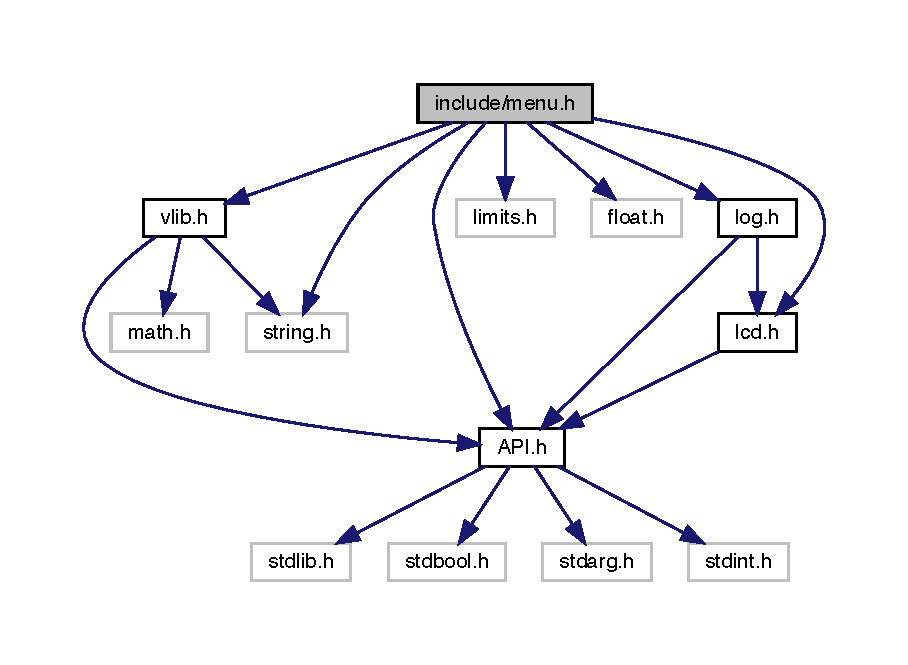
\includegraphics[width=350pt]{menu_8h__incl}
\end{center}
\end{figure}
This graph shows which files directly or indirectly include this file\+:\nopagebreak
\begin{figure}[H]
\begin{center}
\leavevmode
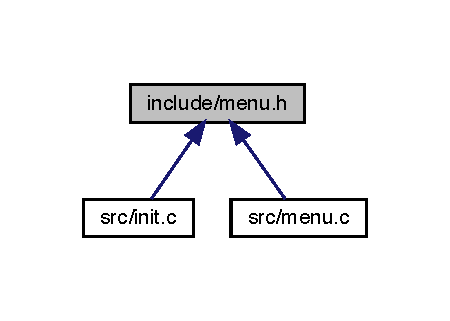
\includegraphics[width=216pt]{menu_8h__dep__incl}
\end{center}
\end{figure}
\subsection*{Data Structures}
\begin{DoxyCompactItemize}
\item 
struct \textbf{ menu\+\_\+t}
\begin{DoxyCompactList}\small\item\em Represents a specific instance of a menu. Will cause a memory leak if not deinitialized via denint\+\_\+menu. \end{DoxyCompactList}\end{DoxyCompactItemize}
\subsection*{Typedefs}
\begin{DoxyCompactItemize}
\item 
typedef struct \textbf{ menu\+\_\+t} \textbf{ menu\+\_\+t}
\begin{DoxyCompactList}\small\item\em Represents a specific instance of a menu. Will cause a memory leak if not deinitialized via denint\+\_\+menu. \end{DoxyCompactList}\end{DoxyCompactItemize}
\subsection*{Enumerations}
\begin{DoxyCompactItemize}
\item 
enum \textbf{ menu\+\_\+type} \{ \textbf{ I\+N\+T\+\_\+\+T\+Y\+PE}, 
\textbf{ F\+L\+O\+A\+T\+\_\+\+T\+Y\+PE}, 
\textbf{ S\+T\+R\+I\+N\+G\+\_\+\+T\+Y\+PE}
 \}\begin{DoxyCompactList}\small\item\em Represents the different types of menus. \end{DoxyCompactList}
\end{DoxyCompactItemize}
\subsection*{Functions}
\begin{DoxyCompactItemize}
\item 
static void \textbf{ calculate\+\_\+current\+\_\+display} (char $\ast$rtn, \textbf{ menu\+\_\+t} $\ast$menu)
\begin{DoxyCompactList}\small\item\em Static function that calculates the string from menu. \end{DoxyCompactList}\item 
static \textbf{ menu\+\_\+t} $\ast$ \textbf{ create\+\_\+menu} (enum \textbf{ menu\+\_\+type} type, const char $\ast$prompt)
\begin{DoxyCompactList}\small\item\em Static function that handles creation of menu. {\itshape  Menu must be freed or will cause memory leak {\itshape  }}\end{DoxyCompactList}\item 
void \textbf{ denint\+\_\+menu} (\textbf{ menu\+\_\+t} $\ast$menu)
\begin{DoxyCompactList}\small\item\em Destroys a menu {\itshape  Menu must be freed or will cause memory leak {\itshape  }}\end{DoxyCompactList}\item 
int \textbf{ display\+\_\+menu} (\textbf{ menu\+\_\+t} $\ast$menu)
\begin{DoxyCompactList}\small\item\em Displays a menu context, but does not display. {\itshape  Menu must be freed or will cause memory leak! {\itshape  Will exit if robot is enabled. This prevents menu from locking up system in even of a reset. }}\end{DoxyCompactList}\item 
\textbf{ menu\+\_\+t} $\ast$ \textbf{ init\+\_\+menu\+\_\+float} (enum \textbf{ menu\+\_\+type} type, float \textbf{ min}, float \textbf{ max}, float step, const char $\ast$prompt)
\begin{DoxyCompactList}\small\item\em Creates a menu context, but does not display. {\itshape  Menu must be freed or will cause memory leak! {\itshape  }}\end{DoxyCompactList}\item 
\textbf{ menu\+\_\+t} $\ast$ \textbf{ init\+\_\+menu\+\_\+int} (enum \textbf{ menu\+\_\+type} type, int \textbf{ min}, int \textbf{ max}, int step, const char $\ast$prompt)
\begin{DoxyCompactList}\small\item\em Creates a menu context, but does not display. {\itshape  Menu must be freed or will cause memory leak {\itshape  }}\end{DoxyCompactList}\item 
\textbf{ menu\+\_\+t} $\ast$ \textbf{ init\+\_\+menu\+\_\+var} (enum \textbf{ menu\+\_\+type} type, unsigned int nums, const char $\ast$prompt, char $\ast$options,...)
\begin{DoxyCompactList}\small\item\em Creates a menu context, but does not display. {\itshape  Menu must be freed or will cause memory leak {\itshape  }}\end{DoxyCompactList}\end{DoxyCompactItemize}


\subsection{Detailed Description}
Contains menu functionality and abstraction. 

\begin{DoxyAuthor}{Author}
Chris Jerrett 
\end{DoxyAuthor}
\begin{DoxyDate}{Date}
9/9/2017 
\end{DoxyDate}


Definition in file \textbf{ menu.\+h}.



\subsection{Typedef Documentation}
\mbox{\label{menu_8h_aac280f147a4bb94ab2f1a69eff76f751}} 
\index{menu.\+h@{menu.\+h}!menu\+\_\+t@{menu\+\_\+t}}
\index{menu\+\_\+t@{menu\+\_\+t}!menu.\+h@{menu.\+h}}
\subsubsection{menu\+\_\+t}
{\footnotesize\ttfamily typedef struct \textbf{ menu\+\_\+t}  \textbf{ menu\+\_\+t}}



Represents a specific instance of a menu. Will cause a memory leak if not deinitialized via denint\+\_\+menu. 

\begin{DoxyAuthor}{Author}
Chris Jerrett 
\end{DoxyAuthor}
\begin{DoxyDate}{Date}
9/8/17 
\end{DoxyDate}
\begin{DoxySeeAlso}{See also}
\doxyref{menu.\+h}{p.}{menu_8h} 

\doxyref{menu\+\_\+t}{p.}{structmenu__t} 

\doxyref{create\+\_\+menu}{p.}{menu_8c_aff4fd27ff7707295d91c67fa52a6b021} 

init\+\_\+menu 

\doxyref{display\+\_\+menu}{p.}{menu_8c_abfadedb104f89f672dd3045499975a71} 

\doxyref{menu\+\_\+type}{p.}{menu_8h_a6bbf4baf5018b0d76aab6c2e6bf85e62} 

\doxyref{denint\+\_\+menu}{p.}{menu_8c_a05a36619ac6c9ba4544eddb83ee2a50d} 
\end{DoxySeeAlso}


\subsection{Enumeration Type Documentation}
\mbox{\label{menu_8h_a6bbf4baf5018b0d76aab6c2e6bf85e62}} 
\index{menu.\+h@{menu.\+h}!menu\+\_\+type@{menu\+\_\+type}}
\index{menu\+\_\+type@{menu\+\_\+type}!menu.\+h@{menu.\+h}}
\subsubsection{menu\+\_\+type}
{\footnotesize\ttfamily enum \textbf{ menu\+\_\+type}}



Represents the different types of menus. 

\begin{DoxyAuthor}{Author}
Chris Jerrett 
\end{DoxyAuthor}
\begin{DoxyDate}{Date}
9/8/17 
\end{DoxyDate}
\begin{DoxySeeAlso}{See also}
\doxyref{menu.\+h}{p.}{menu_8h} 

\doxyref{menu\+\_\+t}{p.}{structmenu__t} 

\doxyref{create\+\_\+menu}{p.}{menu_8h_adcee778eac0edb821427d32949106dc5} 

init\+\_\+menu 

\doxyref{display\+\_\+menu}{p.}{menu_8h_abfadedb104f89f672dd3045499975a71} 

\doxyref{menu\+\_\+type}{p.}{menu_8h_a6bbf4baf5018b0d76aab6c2e6bf85e62} 
\end{DoxySeeAlso}
\begin{DoxyEnumFields}{Enumerator}
\raisebox{\heightof{T}}[0pt][0pt]{\index{I\+N\+T\+\_\+\+T\+Y\+PE@{I\+N\+T\+\_\+\+T\+Y\+PE}!menu.\+h@{menu.\+h}}\index{menu.\+h@{menu.\+h}!I\+N\+T\+\_\+\+T\+Y\+PE@{I\+N\+T\+\_\+\+T\+Y\+PE}}}\mbox{\label{menu_8h_a6bbf4baf5018b0d76aab6c2e6bf85e62a7fee88532b24b79bf2a88688a5d681d7}} 
I\+N\+T\+\_\+\+T\+Y\+PE&Menu type allowing user to select a integer. The integer type menu has a max, min and a step value. Each step is calculated. Will return the index of the selected value. Example\+: User goes forwards twice then it will return 2. \\
\hline

\raisebox{\heightof{T}}[0pt][0pt]{\index{F\+L\+O\+A\+T\+\_\+\+T\+Y\+PE@{F\+L\+O\+A\+T\+\_\+\+T\+Y\+PE}!menu.\+h@{menu.\+h}}\index{menu.\+h@{menu.\+h}!F\+L\+O\+A\+T\+\_\+\+T\+Y\+PE@{F\+L\+O\+A\+T\+\_\+\+T\+Y\+PE}}}\mbox{\label{menu_8h_a6bbf4baf5018b0d76aab6c2e6bf85e62ab2a272a88abadbaa481269e2506345c5}} 
F\+L\+O\+A\+T\+\_\+\+T\+Y\+PE&Menu type allowing user to select a float The float type menu has a max, min and a step value. Each step is calculated. Will return the index of the selected value. Example\+: User goes forwards twice then it will return 2. \\
\hline

\raisebox{\heightof{T}}[0pt][0pt]{\index{S\+T\+R\+I\+N\+G\+\_\+\+T\+Y\+PE@{S\+T\+R\+I\+N\+G\+\_\+\+T\+Y\+PE}!menu.\+h@{menu.\+h}}\index{menu.\+h@{menu.\+h}!S\+T\+R\+I\+N\+G\+\_\+\+T\+Y\+PE@{S\+T\+R\+I\+N\+G\+\_\+\+T\+Y\+PE}}}\mbox{\label{menu_8h_a6bbf4baf5018b0d76aab6c2e6bf85e62a7823190eb356a6edf2f33589f250053c}} 
S\+T\+R\+I\+N\+G\+\_\+\+T\+Y\+PE&Menu type allowing user to select a string from a array of strings. Will return the index of the selected value. Example\+: User goes forwards twice then it will return 2. \\
\hline

\end{DoxyEnumFields}


Definition at line \textbf{ 30} of file \textbf{ menu.\+h}.


\begin{DoxyCode}
00030                \{
00037   INT_TYPE,
00044   FLOAT_TYPE,
00050   STRING_TYPE
00051 \};
\end{DoxyCode}


\subsection{Function Documentation}
\mbox{\label{menu_8h_a0fb55c1213b23963d509b974d1254567}} 
\index{menu.\+h@{menu.\+h}!calculate\+\_\+current\+\_\+display@{calculate\+\_\+current\+\_\+display}}
\index{calculate\+\_\+current\+\_\+display@{calculate\+\_\+current\+\_\+display}!menu.\+h@{menu.\+h}}
\subsubsection{calculate\+\_\+current\+\_\+display()}
{\footnotesize\ttfamily static void calculate\+\_\+current\+\_\+display (\begin{DoxyParamCaption}\item[{char $\ast$}]{rtn,  }\item[{\textbf{ menu\+\_\+t} $\ast$}]{menu }\end{DoxyParamCaption})\hspace{0.3cm}{\ttfamily [static]}}



Static function that calculates the string from menu. 


\begin{DoxyParams}{Parameters}
{\em rtn} & the string to be written to \\
\hline
{\em menu} & the menu for prompt to be calculated from \\
\hline
\end{DoxyParams}
\begin{DoxyAuthor}{Author}
Chris Jerrett 
\end{DoxyAuthor}
\begin{DoxyDate}{Date}
9/8/17 
\end{DoxyDate}
\mbox{\label{menu_8h_adcee778eac0edb821427d32949106dc5}} 
\index{menu.\+h@{menu.\+h}!create\+\_\+menu@{create\+\_\+menu}}
\index{create\+\_\+menu@{create\+\_\+menu}!menu.\+h@{menu.\+h}}
\subsubsection{create\+\_\+menu()}
{\footnotesize\ttfamily static \textbf{ menu\+\_\+t}$\ast$ create\+\_\+menu (\begin{DoxyParamCaption}\item[{enum \textbf{ menu\+\_\+type}}]{type,  }\item[{const char $\ast$}]{prompt }\end{DoxyParamCaption})\hspace{0.3cm}{\ttfamily [static]}}



Static function that handles creation of menu. {\itshape  Menu must be freed or will cause memory leak {\itshape  }}

\begin{DoxyAuthor}{Author}
Chris Jerrett 
\end{DoxyAuthor}
\begin{DoxyDate}{Date}
9/8/17 
\end{DoxyDate}
\mbox{\label{menu_8h_a05a36619ac6c9ba4544eddb83ee2a50d}} 
\index{menu.\+h@{menu.\+h}!denint\+\_\+menu@{denint\+\_\+menu}}
\index{denint\+\_\+menu@{denint\+\_\+menu}!menu.\+h@{menu.\+h}}
\subsubsection{denint\+\_\+menu()}
{\footnotesize\ttfamily void denint\+\_\+menu (\begin{DoxyParamCaption}\item[{\textbf{ menu\+\_\+t} $\ast$}]{menu }\end{DoxyParamCaption})}



Destroys a menu {\itshape  Menu must be freed or will cause memory leak {\itshape  }}


\begin{DoxyParams}{Parameters}
{\em menu} & the menu to free \\
\hline
\end{DoxyParams}
\begin{DoxySeeAlso}{See also}
menu 
\end{DoxySeeAlso}
\begin{DoxyAuthor}{Author}
Chris Jerrett 
\end{DoxyAuthor}
\begin{DoxyDate}{Date}
9/8/17 
\end{DoxyDate}


Definition at line \textbf{ 163} of file \textbf{ menu.\+c}.



References \textbf{ menu\+\_\+t\+::options}, and \textbf{ menu\+\_\+t\+::prompt}.


\begin{DoxyCode}
00163                               \{
00164   free(menu->prompt);
00165   \textcolor{keywordflow}{if}(menu->options != NULL) free(menu->options);
00166   free(menu);
00167 \}
\end{DoxyCode}
\mbox{\label{menu_8h_abfadedb104f89f672dd3045499975a71}} 
\index{menu.\+h@{menu.\+h}!display\+\_\+menu@{display\+\_\+menu}}
\index{display\+\_\+menu@{display\+\_\+menu}!menu.\+h@{menu.\+h}}
\subsubsection{display\+\_\+menu()}
{\footnotesize\ttfamily int display\+\_\+menu (\begin{DoxyParamCaption}\item[{\textbf{ menu\+\_\+t} $\ast$}]{menu }\end{DoxyParamCaption})}



Displays a menu context, but does not display. {\itshape  Menu must be freed or will cause memory leak! {\itshape  Will exit if robot is enabled. This prevents menu from locking up system in even of a reset. }}


\begin{DoxyParams}{Parameters}
{\em menu} & the menu to display \\
\hline
\end{DoxyParams}
\begin{DoxySeeAlso}{See also}
\doxyref{menu\+\_\+type}{p.}{menu_8h_a6bbf4baf5018b0d76aab6c2e6bf85e62} 
\end{DoxySeeAlso}
\begin{DoxyAuthor}{Author}
Chris Jerrett 
\end{DoxyAuthor}
\begin{DoxyDate}{Date}
9/8/17 
\end{DoxyDate}


Definition at line \textbf{ 136} of file \textbf{ menu.\+c}.



References \textbf{ calculate\+\_\+current\+\_\+display()}, \textbf{ menu\+\_\+t\+::current}, \textbf{ lcd\+\_\+get\+\_\+pressed\+\_\+buttons()}, \textbf{ lcd\+\_\+print()}, \textbf{ P\+R\+E\+S\+S\+ED}, \textbf{ menu\+\_\+t\+::prompt}, \textbf{ R\+E\+L\+E\+A\+S\+ED}, and \textbf{ T\+O\+P\+\_\+\+R\+OW}.


\begin{DoxyCode}
00136                               \{
00137   lcd_print(TOP_ROW, menu->prompt);
00138   \textcolor{comment}{//Will exit if teleop or autonomous begin. This is extremely important if robot disconnects or resets.}
00139   \textcolor{keywordflow}{while}(lcd_get_pressed_buttons().middle == RELEASED && !isEnabled()) \{
00140     \textcolor{keywordtype}{char} val[16];
00141     calculate_current_display(val, menu);
00142 
00143     \textcolor{keywordflow}{if}(lcd_get_pressed_buttons().right == PRESSED) \{
00144       menu->current += 1;
00145     \}
00146     \textcolor{keywordflow}{if}(lcd_get_pressed_buttons().left == PRESSED) \{
00147       menu->current -= 1;
00148     \}
00149     delay(500);
00150   \}
00151   \textcolor{keywordflow}{return} menu->current;
00152 \}
\end{DoxyCode}
\mbox{\label{menu_8h_a5abb752733423805f59ef3b92e3c2e57}} 
\index{menu.\+h@{menu.\+h}!init\+\_\+menu\+\_\+float@{init\+\_\+menu\+\_\+float}}
\index{init\+\_\+menu\+\_\+float@{init\+\_\+menu\+\_\+float}!menu.\+h@{menu.\+h}}
\subsubsection{init\+\_\+menu\+\_\+float()}
{\footnotesize\ttfamily \textbf{ menu\+\_\+t}$\ast$ init\+\_\+menu\+\_\+float (\begin{DoxyParamCaption}\item[{enum \textbf{ menu\+\_\+type}}]{type,  }\item[{float}]{min,  }\item[{float}]{max,  }\item[{float}]{step,  }\item[{const char $\ast$}]{prompt }\end{DoxyParamCaption})}



Creates a menu context, but does not display. {\itshape  Menu must be freed or will cause memory leak! {\itshape  }}


\begin{DoxyParams}{Parameters}
{\em type} & the type of menu \\
\hline
\end{DoxyParams}
\begin{DoxySeeAlso}{See also}
\doxyref{menu\+\_\+type}{p.}{menu_8h_a6bbf4baf5018b0d76aab6c2e6bf85e62} 
\end{DoxySeeAlso}

\begin{DoxyParams}{Parameters}
{\em min} & the minimum value \\
\hline
{\em max} & the maximum value \\
\hline
{\em step} & the step value \\
\hline
{\em prompt} & the prompt to display to user \\
\hline
\end{DoxyParams}
\begin{DoxyAuthor}{Author}
Chris Jerrett 
\end{DoxyAuthor}
\begin{DoxyDate}{Date}
9/8/17 
\end{DoxyDate}


Definition at line \textbf{ 92} of file \textbf{ menu.\+c}.



References \textbf{ create\+\_\+menu()}, \textbf{ max()}, \textbf{ menu\+\_\+t\+::max\+\_\+f}, \textbf{ min()}, \textbf{ menu\+\_\+t\+::min\+\_\+f}, and \textbf{ menu\+\_\+t\+::step\+\_\+f}.


\begin{DoxyCode}
00092                                                                                                   \{
00093   menu_t* menu = create_menu(type, prompt);
00094   menu->min_f = min;
00095   menu->max_f = max;
00096   menu->step_f = step;
00097   \textcolor{keywordflow}{return} menu;
00098 \}
\end{DoxyCode}
\mbox{\label{menu_8h_ac8efedba760ec35ebf841ab19543ba5a}} 
\index{menu.\+h@{menu.\+h}!init\+\_\+menu\+\_\+int@{init\+\_\+menu\+\_\+int}}
\index{init\+\_\+menu\+\_\+int@{init\+\_\+menu\+\_\+int}!menu.\+h@{menu.\+h}}
\subsubsection{init\+\_\+menu\+\_\+int()}
{\footnotesize\ttfamily \textbf{ menu\+\_\+t}$\ast$ init\+\_\+menu\+\_\+int (\begin{DoxyParamCaption}\item[{enum \textbf{ menu\+\_\+type}}]{type,  }\item[{int}]{min,  }\item[{int}]{max,  }\item[{int}]{step,  }\item[{const char $\ast$}]{prompt }\end{DoxyParamCaption})}



Creates a menu context, but does not display. {\itshape  Menu must be freed or will cause memory leak {\itshape  }}


\begin{DoxyParams}{Parameters}
{\em type} & the type of menu \\
\hline
\end{DoxyParams}
\begin{DoxySeeAlso}{See also}
\doxyref{menu\+\_\+type}{p.}{menu_8h_a6bbf4baf5018b0d76aab6c2e6bf85e62} 
\end{DoxySeeAlso}

\begin{DoxyParams}{Parameters}
{\em min} & the minimum value \\
\hline
{\em max} & the maximum value \\
\hline
{\em step} & the step value \\
\hline
{\em prompt} & the prompt to display to user \\
\hline
\end{DoxyParams}
\begin{DoxyAuthor}{Author}
Chris Jerrett 
\end{DoxyAuthor}
\begin{DoxyDate}{Date}
9/8/17 
\end{DoxyDate}


Definition at line \textbf{ 71} of file \textbf{ menu.\+c}.



References \textbf{ create\+\_\+menu()}, \textbf{ max()}, \textbf{ menu\+\_\+t\+::max}, \textbf{ min()}, \textbf{ menu\+\_\+t\+::min}, and \textbf{ menu\+\_\+t\+::step}.


\begin{DoxyCode}
00071                                                                                           \{
00072   menu_t* menu = create_menu(type, prompt);
00073   menu->min = min;
00074   menu->max = max;
00075   menu->step = step;
00076   \textcolor{keywordflow}{return} menu;
00077 \}
\end{DoxyCode}
\mbox{\label{menu_8h_a3529988b0a7c12cb3f2ebb3cf5595594}} 
\index{menu.\+h@{menu.\+h}!init\+\_\+menu\+\_\+var@{init\+\_\+menu\+\_\+var}}
\index{init\+\_\+menu\+\_\+var@{init\+\_\+menu\+\_\+var}!menu.\+h@{menu.\+h}}
\subsubsection{init\+\_\+menu\+\_\+var()}
{\footnotesize\ttfamily \textbf{ menu\+\_\+t}$\ast$ init\+\_\+menu\+\_\+var (\begin{DoxyParamCaption}\item[{enum \textbf{ menu\+\_\+type}}]{type,  }\item[{unsigned int}]{nums,  }\item[{const char $\ast$}]{prompt,  }\item[{char $\ast$}]{options,  }\item[{}]{... }\end{DoxyParamCaption})}



Creates a menu context, but does not display. {\itshape  Menu must be freed or will cause memory leak {\itshape  }}


\begin{DoxyParams}{Parameters}
{\em type} & the type of menu \\
\hline
\end{DoxyParams}
\begin{DoxySeeAlso}{See also}
\doxyref{menu\+\_\+type}{p.}{menu_8h_a6bbf4baf5018b0d76aab6c2e6bf85e62} 
\end{DoxySeeAlso}

\begin{DoxyParams}{Parameters}
{\em nums} & the number of elements passed to function \\
\hline
{\em prompt} & the prompt to display to user \\
\hline
{\em options} & the options to display for user \\
\hline
\end{DoxyParams}
\begin{DoxyAuthor}{Author}
Chris Jerrett 
\end{DoxyAuthor}
\begin{DoxyDate}{Date}
9/8/17 
\end{DoxyDate}


Definition at line \textbf{ 44} of file \textbf{ menu.\+c}.



References \textbf{ create\+\_\+menu()}, \textbf{ menu\+\_\+t\+::length}, and \textbf{ menu\+\_\+t\+::options}.


\begin{DoxyCode}
00044                                                                                                     \{
00045   menu_t* menu = create_menu(type, prompt);
00046   va\_list values;
00047   \textcolor{keywordtype}{char} **options\_array = (\textcolor{keywordtype}{char}**)calloc(\textcolor{keyword}{sizeof}(\textcolor{keywordtype}{char}*), nums);
00048   va\_start(values, options);
00049   \textcolor{keywordflow}{for}(\textcolor{keywordtype}{unsigned} \textcolor{keywordtype}{int} i = 0; i < nums; i++)\{
00050     options\_array[i] = va\_arg(values, \textcolor{keywordtype}{char}*);
00051   \}
00052   va\_end(values);
00053   menu->options = options\_array;
00054   menu->length = nums;
00055   \textcolor{keywordflow}{return} menu;
00056 \}
\end{DoxyCode}

\hypertarget{ports_8h}{}\section{include/ports.h File Reference}
\label{ports_8h}\index{include/ports.\+h@{include/ports.\+h}}
\subsection*{Macros}
\begin{DoxyCompactItemize}
\item 
\#define \hyperlink{ports_8h_ae59fbcf599f31d0317338ee35491c175}{I\+M\+E\+\_\+\+F\+R\+O\+N\+T\+\_\+\+R\+I\+G\+HT}~0
\end{DoxyCompactItemize}


\subsection{Macro Definition Documentation}
\mbox{\Hypertarget{ports_8h_ae59fbcf599f31d0317338ee35491c175}\label{ports_8h_ae59fbcf599f31d0317338ee35491c175}} 
\index{ports.\+h@{ports.\+h}!I\+M\+E\+\_\+\+F\+R\+O\+N\+T\+\_\+\+R\+I\+G\+HT@{I\+M\+E\+\_\+\+F\+R\+O\+N\+T\+\_\+\+R\+I\+G\+HT}}
\index{I\+M\+E\+\_\+\+F\+R\+O\+N\+T\+\_\+\+R\+I\+G\+HT@{I\+M\+E\+\_\+\+F\+R\+O\+N\+T\+\_\+\+R\+I\+G\+HT}!ports.\+h@{ports.\+h}}
\subsubsection{\texorpdfstring{I\+M\+E\+\_\+\+F\+R\+O\+N\+T\+\_\+\+R\+I\+G\+HT}{IME\_FRONT\_RIGHT}}
{\footnotesize\ttfamily \#define I\+M\+E\+\_\+\+F\+R\+O\+N\+T\+\_\+\+R\+I\+G\+HT~0}



Definition at line 4 of file ports.\+h.


\hypertarget{slew_8h}{}\section{include/slew.h File Reference}
\label{slew_8h}\index{include/slew.\+h@{include/slew.\+h}}


Contains the slew rate controller wrapper for the motors.  


{\ttfamily \#include $<$A\+P\+I.\+h$>$}\newline
{\ttfamily \#include $<$math.\+h$>$}\newline
{\ttfamily \#include $<$vlib.\+h$>$}\newline
Include dependency graph for slew.\+h\+:\nopagebreak
\begin{figure}[H]
\begin{center}
\leavevmode
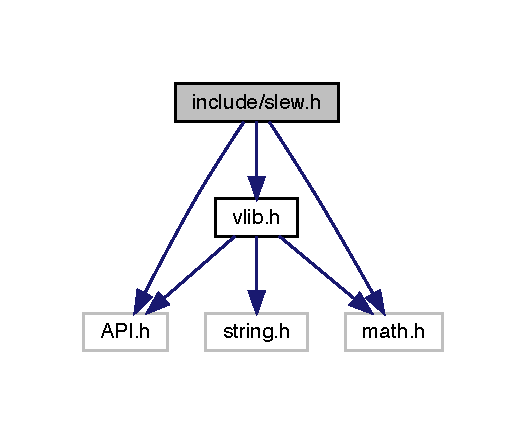
\includegraphics[width=350pt]{slew_8h__incl}
\end{center}
\end{figure}
This graph shows which files directly or indirectly include this file\+:\nopagebreak
\begin{figure}[H]
\begin{center}
\leavevmode
\includegraphics[width=350pt]{slew_8h__dep__incl}
\end{center}
\end{figure}
\subsection*{Macros}
\begin{DoxyCompactItemize}
\item 
\#define \hyperlink{slew_8h_ad1ad4b29af4180aa00713599367fbc98}{M\+O\+T\+O\+R\+\_\+\+P\+O\+R\+TS}~12
\begin{DoxyCompactList}\small\item\em The number of motor ports on the robot. \end{DoxyCompactList}\item 
\#define \hyperlink{slew_8h_a4a3ff8667251227c99f8f4c81e9ff467}{R\+A\+M\+P\+\_\+\+P\+R\+O\+P\+O\+R\+T\+I\+ON}~1
\begin{DoxyCompactList}\small\item\em proportion defining how quickly the motor should converge on the correct value. higher value leads to slower convergence \end{DoxyCompactList}\item 
\#define \hyperlink{slew_8h_a4e8e7d6fdd1f5c6f8a0f341e4b61f025}{U\+P\+D\+A\+T\+E\+\_\+\+P\+E\+R\+I\+O\+D\+\_\+\+MS}~25
\begin{DoxyCompactList}\small\item\em How frequently to update the motors, in milliseconds. \end{DoxyCompactList}\end{DoxyCompactItemize}
\subsection*{Functions}
\begin{DoxyCompactItemize}
\item 
void \hyperlink{slew_8h_a981c9990a969d2587e66e550737f7cd9}{deinitslew} ()
\begin{DoxyCompactList}\small\item\em Deinitializes the slew rate controller and frees memory. \end{DoxyCompactList}\item 
void \hyperlink{slew_8h_a321758941d88b75783955c819bb75005}{init\+\_\+slew} ()
\begin{DoxyCompactList}\small\item\em Initializes the slew rate controller. \end{DoxyCompactList}\item 
void \hyperlink{slew_8h_a9f8b8ae577ef938622024545711f0151}{set\+\_\+motor\+\_\+immediate} (int motor, int speed)
\item 
void \hyperlink{slew_8h_a7dff2b79dffe55fb936d977594d7c01d}{set\+\_\+motor\+\_\+slew} (int motor, int speed)
\begin{DoxyCompactList}\small\item\em Sets motor speed wrapped inside the slew rate controller. \end{DoxyCompactList}\item 
void \hyperlink{slew_8h_a807a87c5df438fde21c1e8213906695b}{update\+Motors} ()
\begin{DoxyCompactList}\small\item\em Closes the distance between the desired motor value and the current motor value by half for each motor. \end{DoxyCompactList}\end{DoxyCompactItemize}


\subsection{Detailed Description}
Contains the slew rate controller wrapper for the motors. 

\begin{DoxyAuthor}{Author}
Chris Jerrett 
\end{DoxyAuthor}
\begin{DoxyDate}{Date}
9/14/17 
\end{DoxyDate}


\subsection{Macro Definition Documentation}
\mbox{\Hypertarget{slew_8h_ad1ad4b29af4180aa00713599367fbc98}\label{slew_8h_ad1ad4b29af4180aa00713599367fbc98}} 
\index{slew.\+h@{slew.\+h}!M\+O\+T\+O\+R\+\_\+\+P\+O\+R\+TS@{M\+O\+T\+O\+R\+\_\+\+P\+O\+R\+TS}}
\index{M\+O\+T\+O\+R\+\_\+\+P\+O\+R\+TS@{M\+O\+T\+O\+R\+\_\+\+P\+O\+R\+TS}!slew.\+h@{slew.\+h}}
\subsubsection{\texorpdfstring{M\+O\+T\+O\+R\+\_\+\+P\+O\+R\+TS}{MOTOR\_PORTS}}
{\footnotesize\ttfamily \#define M\+O\+T\+O\+R\+\_\+\+P\+O\+R\+TS~12}



The number of motor ports on the robot. 

\begin{DoxyAuthor}{Author}
Christian De\+Simone 
\end{DoxyAuthor}
\begin{DoxyDate}{Date}
9/14/17 
\end{DoxyDate}


Definition at line 27 of file slew.\+h.

\mbox{\Hypertarget{slew_8h_a4a3ff8667251227c99f8f4c81e9ff467}\label{slew_8h_a4a3ff8667251227c99f8f4c81e9ff467}} 
\index{slew.\+h@{slew.\+h}!R\+A\+M\+P\+\_\+\+P\+R\+O\+P\+O\+R\+T\+I\+ON@{R\+A\+M\+P\+\_\+\+P\+R\+O\+P\+O\+R\+T\+I\+ON}}
\index{R\+A\+M\+P\+\_\+\+P\+R\+O\+P\+O\+R\+T\+I\+ON@{R\+A\+M\+P\+\_\+\+P\+R\+O\+P\+O\+R\+T\+I\+ON}!slew.\+h@{slew.\+h}}
\subsubsection{\texorpdfstring{R\+A\+M\+P\+\_\+\+P\+R\+O\+P\+O\+R\+T\+I\+ON}{RAMP\_PROPORTION}}
{\footnotesize\ttfamily \#define R\+A\+M\+P\+\_\+\+P\+R\+O\+P\+O\+R\+T\+I\+ON~1}



proportion defining how quickly the motor should converge on the correct value. higher value leads to slower convergence 

\begin{DoxyAuthor}{Author}
Chris Jerrett 
\end{DoxyAuthor}
\begin{DoxyDate}{Date}
9/14/17 
\end{DoxyDate}


Definition at line 34 of file slew.\+h.

\mbox{\Hypertarget{slew_8h_a4e8e7d6fdd1f5c6f8a0f341e4b61f025}\label{slew_8h_a4e8e7d6fdd1f5c6f8a0f341e4b61f025}} 
\index{slew.\+h@{slew.\+h}!U\+P\+D\+A\+T\+E\+\_\+\+P\+E\+R\+I\+O\+D\+\_\+\+MS@{U\+P\+D\+A\+T\+E\+\_\+\+P\+E\+R\+I\+O\+D\+\_\+\+MS}}
\index{U\+P\+D\+A\+T\+E\+\_\+\+P\+E\+R\+I\+O\+D\+\_\+\+MS@{U\+P\+D\+A\+T\+E\+\_\+\+P\+E\+R\+I\+O\+D\+\_\+\+MS}!slew.\+h@{slew.\+h}}
\subsubsection{\texorpdfstring{U\+P\+D\+A\+T\+E\+\_\+\+P\+E\+R\+I\+O\+D\+\_\+\+MS}{UPDATE\_PERIOD\_MS}}
{\footnotesize\ttfamily \#define U\+P\+D\+A\+T\+E\+\_\+\+P\+E\+R\+I\+O\+D\+\_\+\+MS~25}



How frequently to update the motors, in milliseconds. 

\begin{DoxyAuthor}{Author}
Chris Jerrett 
\end{DoxyAuthor}
\begin{DoxyDate}{Date}
9/14/17 
\end{DoxyDate}


Definition at line 20 of file slew.\+h.



\subsection{Function Documentation}
\mbox{\Hypertarget{slew_8h_a981c9990a969d2587e66e550737f7cd9}\label{slew_8h_a981c9990a969d2587e66e550737f7cd9}} 
\index{slew.\+h@{slew.\+h}!deinitslew@{deinitslew}}
\index{deinitslew@{deinitslew}!slew.\+h@{slew.\+h}}
\subsubsection{\texorpdfstring{deinitslew()}{deinitslew()}}
{\footnotesize\ttfamily void deinitslew (\begin{DoxyParamCaption}{ }\end{DoxyParamCaption})}



Deinitializes the slew rate controller and frees memory. 

\begin{DoxyAuthor}{Author}
Chris Jerrett 
\end{DoxyAuthor}
\begin{DoxyDate}{Date}
9/14/17 
\end{DoxyDate}


Definition at line 43 of file slew.\+c.



References initialized, motors\+\_\+curr\+\_\+speeds, motors\+\_\+set\+\_\+speeds, slew, and task\+Delete().



Referenced by autonomous().


\begin{DoxyCode}
43                  \{
44   \hyperlink{_a_p_i_8h_add3b8d580ea6ef5635c6d9ff88c68612}{taskDelete}(\hyperlink{slew_8c_a9dc30877eadbb32ceb6bede027c9a93f}{slew});
45   memset(\hyperlink{slew_8c_acf7558ed17fdecd298ea7eb82291c7d0}{motors\_set\_speeds}, 0, \textcolor{keyword}{sizeof}(\textcolor{keywordtype}{int}) * 10);
46   memset(\hyperlink{slew_8c_a69e0d1204ea4d87b7366c9cd79527984}{motors\_curr\_speeds}, 0, \textcolor{keyword}{sizeof}(\textcolor{keywordtype}{int}) * 10);
47   \hyperlink{slew_8c_aedeffc7d23da25d52b9a50045189fe2b}{initialized} = \textcolor{keyword}{false};
48 \}
\end{DoxyCode}
Here is the call graph for this function\+:\nopagebreak
\begin{figure}[H]
\begin{center}
\leavevmode
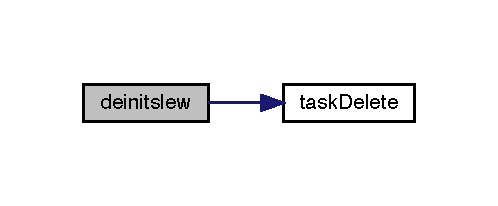
\includegraphics[width=239pt]{slew_8h_a981c9990a969d2587e66e550737f7cd9_cgraph}
\end{center}
\end{figure}
Here is the caller graph for this function\+:\nopagebreak
\begin{figure}[H]
\begin{center}
\leavevmode
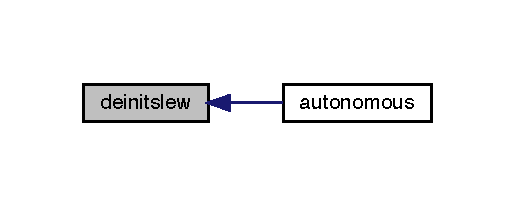
\includegraphics[width=247pt]{slew_8h_a981c9990a969d2587e66e550737f7cd9_icgraph}
\end{center}
\end{figure}
\mbox{\Hypertarget{slew_8h_a321758941d88b75783955c819bb75005}\label{slew_8h_a321758941d88b75783955c819bb75005}} 
\index{slew.\+h@{slew.\+h}!init\+\_\+slew@{init\+\_\+slew}}
\index{init\+\_\+slew@{init\+\_\+slew}!slew.\+h@{slew.\+h}}
\subsubsection{\texorpdfstring{init\+\_\+slew()}{init\_slew()}}
{\footnotesize\ttfamily void init\+\_\+slew (\begin{DoxyParamCaption}{ }\end{DoxyParamCaption})}



Initializes the slew rate controller. 

\begin{DoxyAuthor}{Author}
Chris Jerrett, Christian De\+Simone 
\end{DoxyAuthor}
\begin{DoxyDate}{Date}
9/14/17 
\end{DoxyDate}


Definition at line 30 of file slew.\+c.



References info(), initialized, motors\+\_\+curr\+\_\+speeds, motors\+\_\+set\+\_\+speeds, motor\+Stop\+All(), mutex\+Create(), slew, speeds\+\_\+mutex, task\+Run\+Loop(), update\+Motors(), and warning().



Referenced by autonomous(), operator\+Control(), set\+\_\+motor\+\_\+immediate(), and set\+\_\+motor\+\_\+slew().


\begin{DoxyCode}
30                 \{
31   \textcolor{keywordflow}{if}(\hyperlink{slew_8c_aedeffc7d23da25d52b9a50045189fe2b}{initialized}) \{
32     \hyperlink{log_8h_a0bec2cf5fff7f607bc510b74aba9887c}{warning}(\textcolor{stringliteral}{"Trying to init already init slew"});
33   \}
34   memset(\hyperlink{slew_8c_acf7558ed17fdecd298ea7eb82291c7d0}{motors\_set\_speeds}, 0, \textcolor{keyword}{sizeof}(\textcolor{keywordtype}{int}) * 10);
35   memset(\hyperlink{slew_8c_a69e0d1204ea4d87b7366c9cd79527984}{motors\_curr\_speeds}, 0, \textcolor{keyword}{sizeof}(\textcolor{keywordtype}{int}) * 10);
36   \hyperlink{_a_p_i_8h_a8966c541f3e9565aea1289f0d2f2cf43}{motorStopAll}();
37   \hyperlink{log_8h_a1606d750e1bb8de9f9e917172bba3382}{info}(\textcolor{stringliteral}{"Did Init Slew"});
38   \hyperlink{slew_8c_a29ddd4c66a52ff81b441d04f9f6d9318}{speeds\_mutex} = \hyperlink{_a_p_i_8h_aecd027ce8f8b52a765735e9eb5b202b3}{mutexCreate}();
39   \hyperlink{slew_8c_a9dc30877eadbb32ceb6bede027c9a93f}{slew} = \hyperlink{_a_p_i_8h_ab05a241d6d1fd98b1ceb4665db678156}{taskRunLoop}(\hyperlink{slew_8c_a807a87c5df438fde21c1e8213906695b}{updateMotors}, 100);
40   \hyperlink{slew_8c_aedeffc7d23da25d52b9a50045189fe2b}{initialized} = \textcolor{keyword}{true};
41 \}
\end{DoxyCode}
Here is the call graph for this function\+:\nopagebreak
\begin{figure}[H]
\begin{center}
\leavevmode
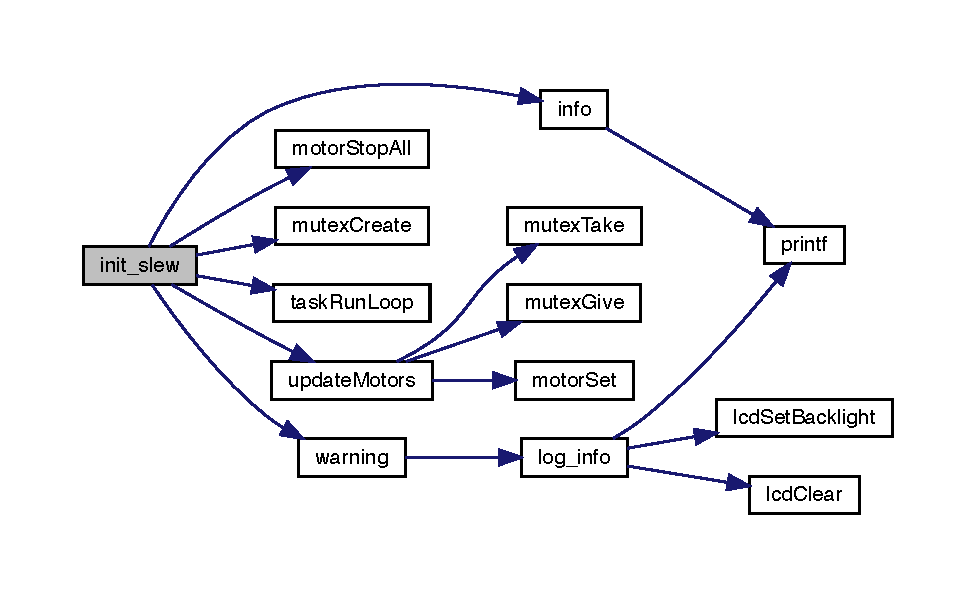
\includegraphics[width=350pt]{slew_8h_a321758941d88b75783955c819bb75005_cgraph}
\end{center}
\end{figure}
Here is the caller graph for this function\+:\nopagebreak
\begin{figure}[H]
\begin{center}
\leavevmode
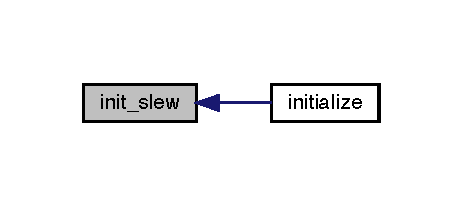
\includegraphics[width=350pt]{slew_8h_a321758941d88b75783955c819bb75005_icgraph}
\end{center}
\end{figure}
\mbox{\Hypertarget{slew_8h_a9f8b8ae577ef938622024545711f0151}\label{slew_8h_a9f8b8ae577ef938622024545711f0151}} 
\index{slew.\+h@{slew.\+h}!set\+\_\+motor\+\_\+immediate@{set\+\_\+motor\+\_\+immediate}}
\index{set\+\_\+motor\+\_\+immediate@{set\+\_\+motor\+\_\+immediate}!slew.\+h@{slew.\+h}}
\subsubsection{\texorpdfstring{set\+\_\+motor\+\_\+immediate()}{set\_motor\_immediate()}}
{\footnotesize\ttfamily void set\+\_\+motor\+\_\+immediate (\begin{DoxyParamCaption}\item[{int}]{motor,  }\item[{int}]{speed }\end{DoxyParamCaption})}



Definition at line 60 of file slew.\+c.



References debug(), init\+\_\+slew(), initialized, motors\+\_\+curr\+\_\+speeds, motors\+\_\+set\+\_\+speeds, motor\+Set(), mutex\+Give(), mutex\+Take(), and speeds\+\_\+mutex.



Referenced by close\+\_\+claw(), open\+\_\+claw(), set\+\_\+claw\+\_\+motor(), set\+\_\+intake\+\_\+motor(), and set\+\_\+lifter\+\_\+motors().


\begin{DoxyCode}
60                                                \{
61   \textcolor{keywordflow}{if}(!\hyperlink{slew_8c_aedeffc7d23da25d52b9a50045189fe2b}{initialized}) \{
62     \hyperlink{log_8h_af3668f40d1ad1b4f3418869ac9a31f34}{debug}(\textcolor{stringliteral}{"Slew Not Initialized! Initializing"});
63     \hyperlink{slew_8c_a321758941d88b75783955c819bb75005}{init\_slew}();
64   \}
65   \hyperlink{_a_p_i_8h_a03c5b04b472d024281f62d7af8854a8e}{motorSet}(motor, speed);
66   \hyperlink{_a_p_i_8h_a8b51124628d2a7741738d48551d1e8ee}{mutexTake}(\hyperlink{slew_8c_a29ddd4c66a52ff81b441d04f9f6d9318}{speeds\_mutex}, 10);
67   \hyperlink{slew_8c_a69e0d1204ea4d87b7366c9cd79527984}{motors\_curr\_speeds}[motor-1] = speed;
68   \hyperlink{slew_8c_acf7558ed17fdecd298ea7eb82291c7d0}{motors\_set\_speeds}[motor-1] = speed;
69   \hyperlink{_a_p_i_8h_afe171a08d22de18fc2ab604b2364959f}{mutexGive}(\hyperlink{slew_8c_a29ddd4c66a52ff81b441d04f9f6d9318}{speeds\_mutex});
70 \}
\end{DoxyCode}
Here is the call graph for this function\+:\nopagebreak
\begin{figure}[H]
\begin{center}
\leavevmode
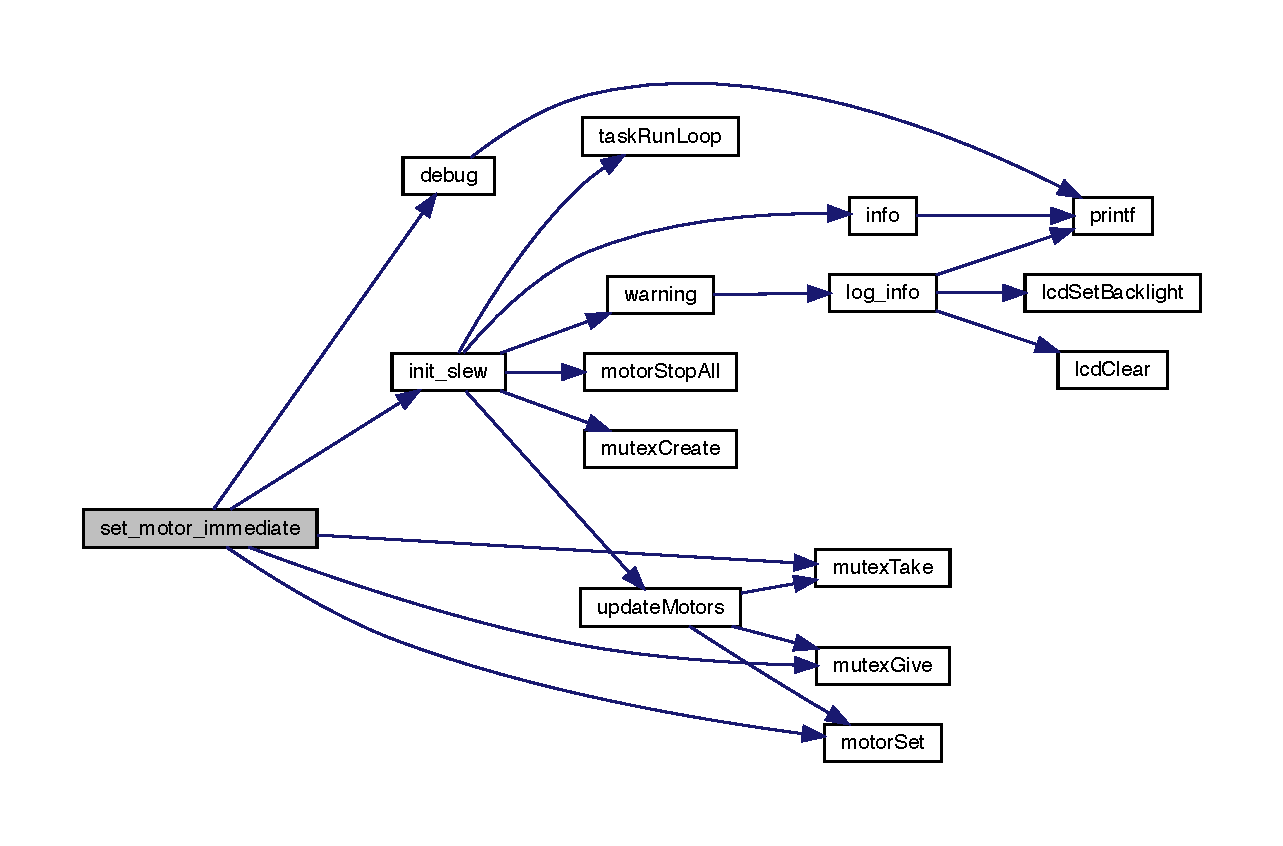
\includegraphics[width=350pt]{slew_8h_a9f8b8ae577ef938622024545711f0151_cgraph}
\end{center}
\end{figure}
Here is the caller graph for this function\+:\nopagebreak
\begin{figure}[H]
\begin{center}
\leavevmode
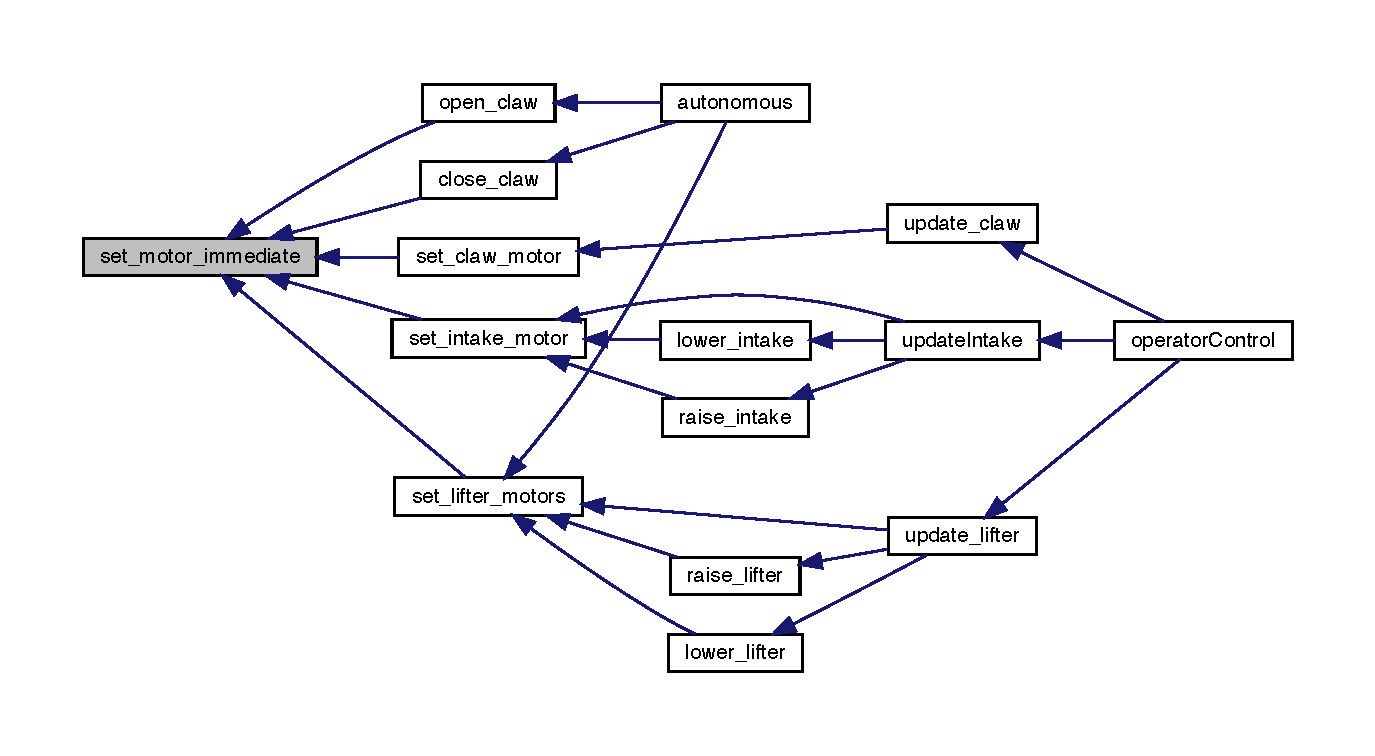
\includegraphics[width=350pt]{slew_8h_a9f8b8ae577ef938622024545711f0151_icgraph}
\end{center}
\end{figure}
\mbox{\Hypertarget{slew_8h_a7dff2b79dffe55fb936d977594d7c01d}\label{slew_8h_a7dff2b79dffe55fb936d977594d7c01d}} 
\index{slew.\+h@{slew.\+h}!set\+\_\+motor\+\_\+slew@{set\+\_\+motor\+\_\+slew}}
\index{set\+\_\+motor\+\_\+slew@{set\+\_\+motor\+\_\+slew}!slew.\+h@{slew.\+h}}
\subsubsection{\texorpdfstring{set\+\_\+motor\+\_\+slew()}{set\_motor\_slew()}}
{\footnotesize\ttfamily void set\+\_\+motor\+\_\+slew (\begin{DoxyParamCaption}\item[{int}]{motor,  }\item[{int}]{speed }\end{DoxyParamCaption})}



Sets motor speed wrapped inside the slew rate controller. 


\begin{DoxyParams}{Parameters}
{\em motor} & the motor port to use \\
\hline
{\em speed} & the speed to use, between -\/127 and 127 \\
\hline
\end{DoxyParams}
\begin{DoxyAuthor}{Author}
Chris Jerrett 
\end{DoxyAuthor}
\begin{DoxyDate}{Date}
9/14/17 
\end{DoxyDate}


Definition at line 50 of file slew.\+c.



References debug(), init\+\_\+slew(), initialized, motors\+\_\+set\+\_\+speeds, mutex\+Give(), mutex\+Take(), and speeds\+\_\+mutex.



Referenced by set\+\_\+side\+\_\+speed().


\begin{DoxyCode}
50                                          \{
51   \textcolor{keywordflow}{if}(!\hyperlink{slew_8c_aedeffc7d23da25d52b9a50045189fe2b}{initialized}) \{
52     \hyperlink{log_8h_af3668f40d1ad1b4f3418869ac9a31f34}{debug}(\textcolor{stringliteral}{"Slew Not Initialized! Initializing"});
53     \hyperlink{slew_8c_a321758941d88b75783955c819bb75005}{init\_slew}();
54   \}
55   \hyperlink{_a_p_i_8h_a8b51124628d2a7741738d48551d1e8ee}{mutexTake}(\hyperlink{slew_8c_a29ddd4c66a52ff81b441d04f9f6d9318}{speeds\_mutex}, 10);
56   \hyperlink{slew_8c_acf7558ed17fdecd298ea7eb82291c7d0}{motors\_set\_speeds}[motor-1] = speed;
57   \hyperlink{_a_p_i_8h_afe171a08d22de18fc2ab604b2364959f}{mutexGive}(\hyperlink{slew_8c_a29ddd4c66a52ff81b441d04f9f6d9318}{speeds\_mutex});
58 \}
\end{DoxyCode}
Here is the call graph for this function\+:\nopagebreak
\begin{figure}[H]
\begin{center}
\leavevmode
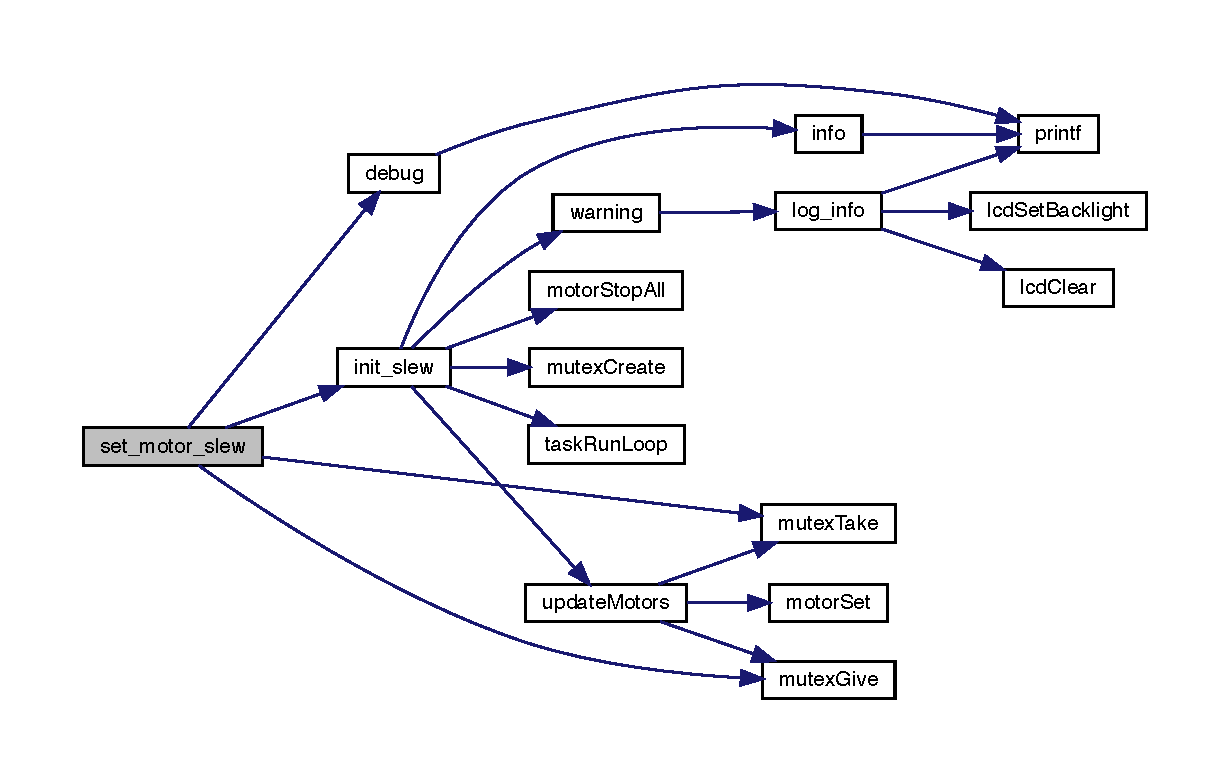
\includegraphics[width=350pt]{slew_8h_a7dff2b79dffe55fb936d977594d7c01d_cgraph}
\end{center}
\end{figure}
Here is the caller graph for this function\+:\nopagebreak
\begin{figure}[H]
\begin{center}
\leavevmode
\includegraphics[width=350pt]{slew_8h_a7dff2b79dffe55fb936d977594d7c01d_icgraph}
\end{center}
\end{figure}
\mbox{\Hypertarget{slew_8h_a807a87c5df438fde21c1e8213906695b}\label{slew_8h_a807a87c5df438fde21c1e8213906695b}} 
\index{slew.\+h@{slew.\+h}!update\+Motors@{update\+Motors}}
\index{update\+Motors@{update\+Motors}!slew.\+h@{slew.\+h}}
\subsubsection{\texorpdfstring{update\+Motors()}{updateMotors()}}
{\footnotesize\ttfamily void update\+Motors (\begin{DoxyParamCaption}{ }\end{DoxyParamCaption})}



Closes the distance between the desired motor value and the current motor value by half for each motor. 

\begin{DoxyAuthor}{Author}
Chris Jerrett 
\end{DoxyAuthor}
\begin{DoxyDate}{Date}
9/14/17 
\end{DoxyDate}


Definition at line 13 of file slew.\+c.



References motors\+\_\+curr\+\_\+speeds, motors\+\_\+set\+\_\+speeds, motor\+Set(), mutex\+Give(), mutex\+Take(), and speeds\+\_\+mutex.



Referenced by init\+\_\+slew().


\begin{DoxyCode}
13                    \{
14   \textcolor{comment}{//Take back half approach}
15   \textcolor{comment}{//Not linear but equal to setSpeed(1-(1/2)^x)}
16   \textcolor{keywordflow}{for}(\textcolor{keywordtype}{unsigned} \textcolor{keywordtype}{int} i = 0; i < 9; i++) \{
17     \textcolor{keywordflow}{if}(\hyperlink{slew_8c_acf7558ed17fdecd298ea7eb82291c7d0}{motors\_set\_speeds}[i] == \hyperlink{slew_8c_a69e0d1204ea4d87b7366c9cd79527984}{motors\_curr\_speeds}[i]) \textcolor{keywordflow}{continue};
18     \hyperlink{_a_p_i_8h_a8b51124628d2a7741738d48551d1e8ee}{mutexTake}(\hyperlink{slew_8c_a29ddd4c66a52ff81b441d04f9f6d9318}{speeds\_mutex}, 10);
19     \textcolor{keywordtype}{int} set\_speed = (\hyperlink{slew_8c_acf7558ed17fdecd298ea7eb82291c7d0}{motors\_set\_speeds}[i]);
20     \textcolor{keywordtype}{int} curr\_speed = \hyperlink{slew_8c_a69e0d1204ea4d87b7366c9cd79527984}{motors\_curr\_speeds}[i];
21     \hyperlink{_a_p_i_8h_afe171a08d22de18fc2ab604b2364959f}{mutexGive}(\hyperlink{slew_8c_a29ddd4c66a52ff81b441d04f9f6d9318}{speeds\_mutex});
22     \textcolor{keywordtype}{int} diff = set\_speed - curr\_speed;
23     \textcolor{keywordtype}{int} offset = diff;
24     \textcolor{keywordtype}{int} n = curr\_speed + offset;
25     \hyperlink{slew_8c_a69e0d1204ea4d87b7366c9cd79527984}{motors\_curr\_speeds}[i] = n;
26     \hyperlink{_a_p_i_8h_a03c5b04b472d024281f62d7af8854a8e}{motorSet}(i+1, n);
27   \}
28 \}
\end{DoxyCode}
Here is the call graph for this function\+:\nopagebreak
\begin{figure}[H]
\begin{center}
\leavevmode
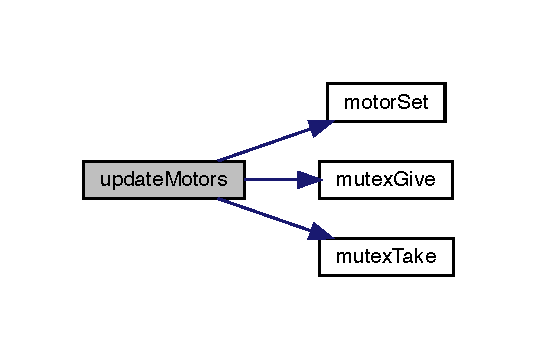
\includegraphics[width=258pt]{slew_8h_a807a87c5df438fde21c1e8213906695b_cgraph}
\end{center}
\end{figure}
Here is the caller graph for this function\+:\nopagebreak
\begin{figure}[H]
\begin{center}
\leavevmode
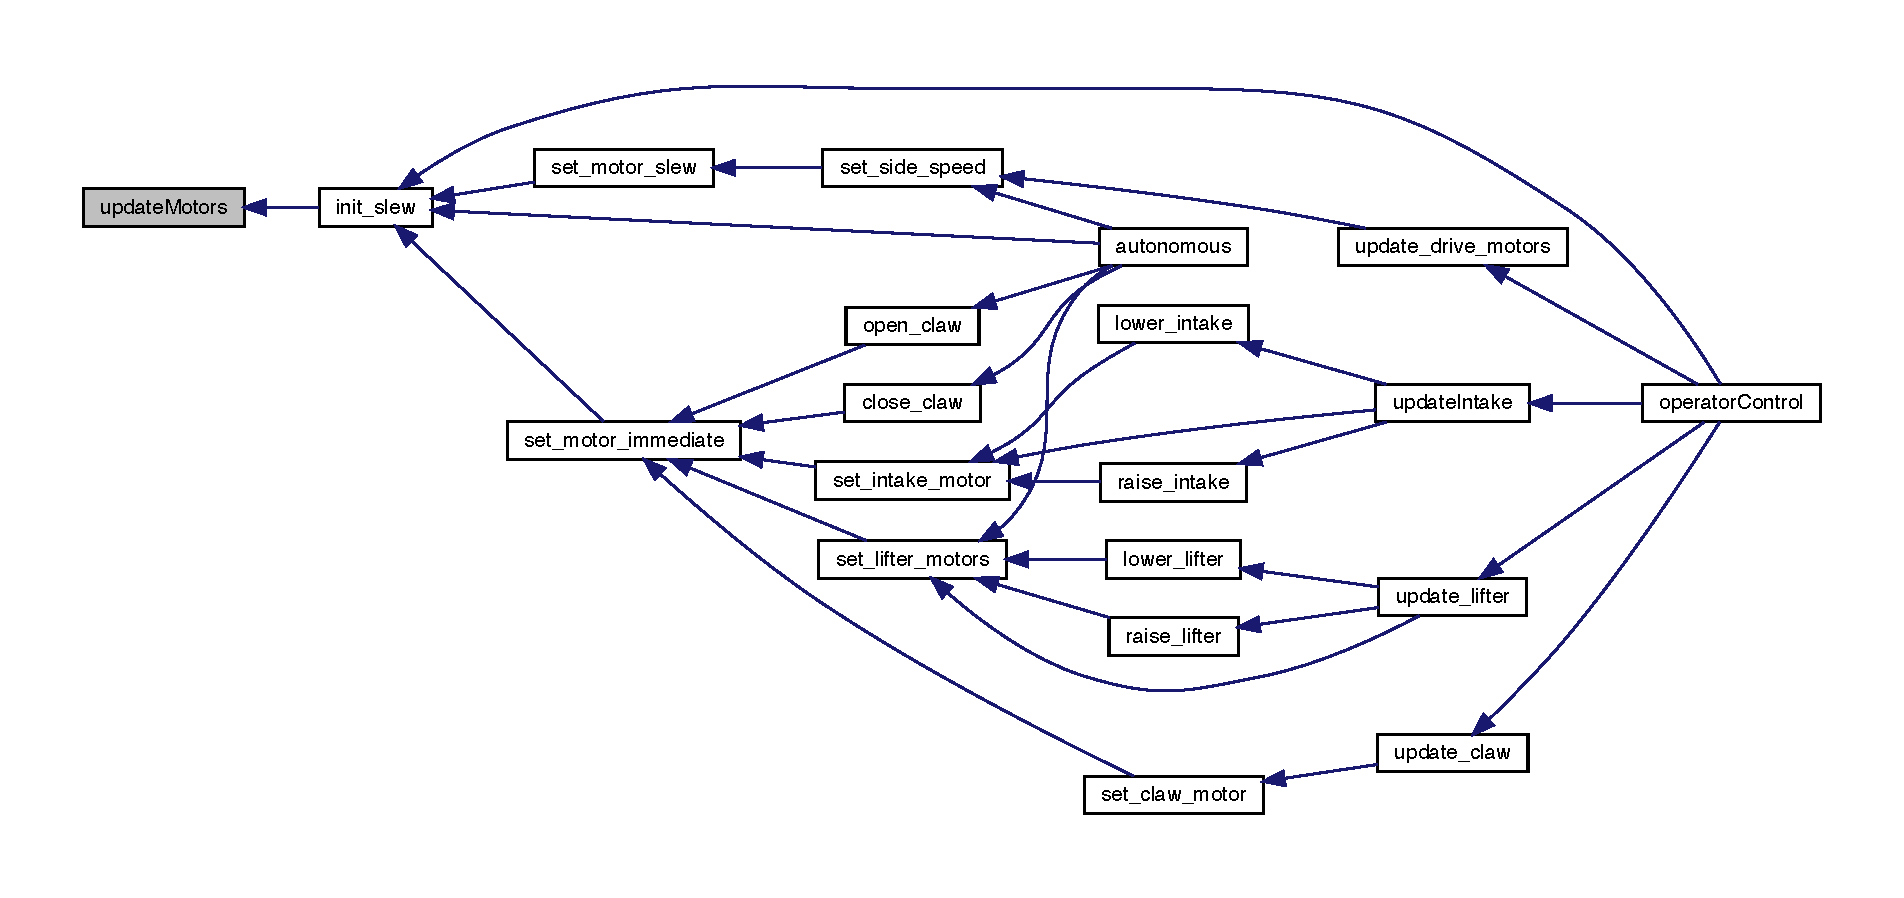
\includegraphics[width=350pt]{slew_8h_a807a87c5df438fde21c1e8213906695b_icgraph}
\end{center}
\end{figure}

\subsection{include/vlib.h File Reference}
\label{vlib_8h}\index{include/vlib.\+h@{include/vlib.\+h}}


Contains misc helpful functions.  


{\ttfamily \#include $<$math.\+h$>$}\newline
{\ttfamily \#include $<$A\+P\+I.\+h$>$}\newline
{\ttfamily \#include $<$string.\+h$>$}\newline
Include dependency graph for vlib.\+h\+:\nopagebreak
\begin{figure}[H]
\begin{center}
\leavevmode
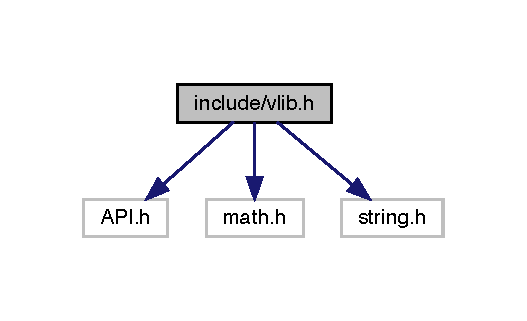
\includegraphics[width=338pt]{vlib_8h__incl}
\end{center}
\end{figure}
This graph shows which files directly or indirectly include this file\+:\nopagebreak
\begin{figure}[H]
\begin{center}
\leavevmode
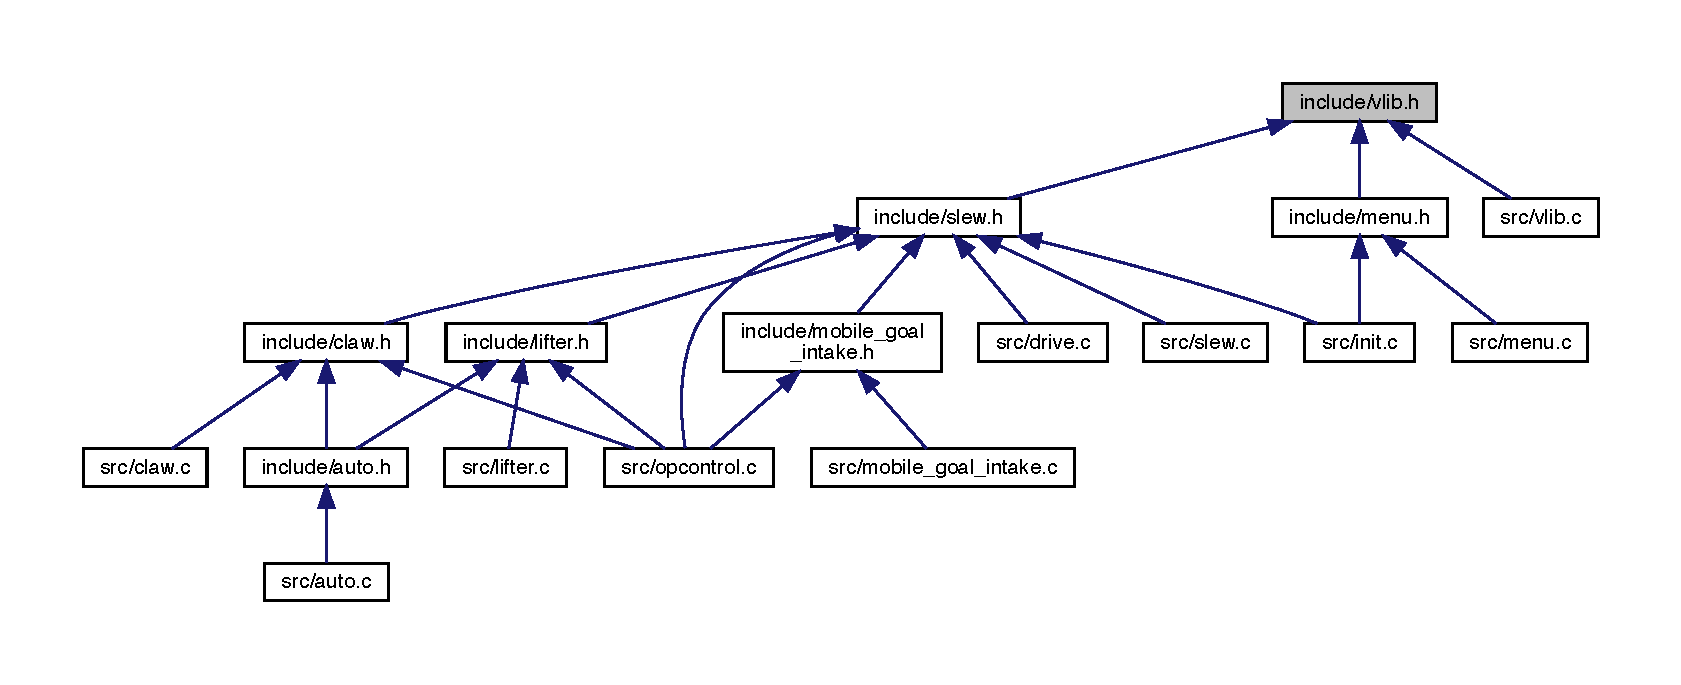
\includegraphics[width=350pt]{vlib_8h__dep__incl}
\end{center}
\end{figure}
\subsubsection*{Functions}
\begin{DoxyCompactItemize}
\item 
void \textbf{ ftoa\+\_\+bad} (float a, char $\ast$buffer, int precision)
\begin{DoxyCompactList}\small\item\em converts a float to string. \end{DoxyCompactList}\item 
int \textbf{ itoa\+\_\+bad} (int a, char $\ast$buffer, int digits)
\begin{DoxyCompactList}\small\item\em converts a int to string. \end{DoxyCompactList}\item 
void \textbf{ reverse} (char $\ast$str, int len)
\begin{DoxyCompactList}\small\item\em reverses a string \textquotesingle{}str\textquotesingle{} of length \textquotesingle{}len\textquotesingle{} \end{DoxyCompactList}\end{DoxyCompactItemize}


\subsubsection{Detailed Description}
Contains misc helpful functions. 

\begin{DoxyAuthor}{Author}
Chris Jerrett 
\end{DoxyAuthor}
\begin{DoxyDate}{Date}
9/9/2017 
\end{DoxyDate}


Definition in file \textbf{ vlib.\+h}.



\subsubsection{Function Documentation}
\mbox{\label{vlib_8h_a8805990ed667939e615e4a98950b8bd1}} 
\index{vlib.\+h@{vlib.\+h}!ftoa\+\_\+bad@{ftoa\+\_\+bad}}
\index{ftoa\+\_\+bad@{ftoa\+\_\+bad}!vlib.\+h@{vlib.\+h}}
\paragraph{ftoa\+\_\+bad()}
{\footnotesize\ttfamily void ftoa\+\_\+bad (\begin{DoxyParamCaption}\item[{float}]{a,  }\item[{char $\ast$}]{buffer,  }\item[{int}]{precision }\end{DoxyParamCaption})}



converts a float to string. 


\begin{DoxyParams}{Parameters}
{\em a} & the float \\
\hline
{\em buffer} & the string the float will be written to. \\
\hline
{\em precision} & digits after the decimal to write \\
\hline
\end{DoxyParams}
\begin{DoxyAuthor}{Author}
Christian De\+Simone 
\end{DoxyAuthor}
\begin{DoxyDate}{Date}
9/26/2017 
\end{DoxyDate}


Definition at line \textbf{ 30} of file \textbf{ vlib.\+c}.



References \textbf{ itoa\+\_\+bad()}.



Referenced by \textbf{ calculate\+\_\+current\+\_\+display()}.


\begin{DoxyCode}
00030                                                     \{
00031   \textcolor{comment}{// Extract integer part}
00032   \textcolor{keywordtype}{int} ipart = (int)a;
00033 
00034   \textcolor{comment}{// Extract floating part}
00035   \textcolor{keywordtype}{float} fpart = a - (float)ipart;
00036 
00037   \textcolor{comment}{// convert integer part to string}
00038   \textcolor{keywordtype}{int} i = itoa_bad(ipart, buffer, 0);
00039 
00040   \textcolor{comment}{// check for display option after point}
00041   \textcolor{keywordflow}{if}(precision != 0) \{
00042     buffer[i] = \textcolor{charliteral}{'.'};  \textcolor{comment}{// add dot}
00043 
00044     \textcolor{comment}{// Get the value of fraction part up to given num.}
00045     \textcolor{comment}{// of points after dot. The third parameter is needed}
00046     \textcolor{comment}{// to handle cases like 233.007}
00047     fpart = fpart * pow(10, precision);
00048 
00049     itoa_bad((\textcolor{keywordtype}{int})fpart, buffer + i + 1, precision);
00050   \}
00051 \}
\end{DoxyCode}
Here is the call graph for this function\+:\nopagebreak
\begin{figure}[H]
\begin{center}
\leavevmode
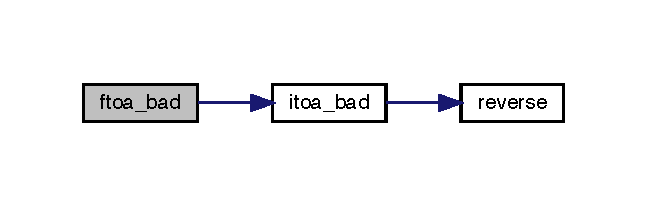
\includegraphics[width=311pt]{vlib_8h_a8805990ed667939e615e4a98950b8bd1_cgraph}
\end{center}
\end{figure}
Here is the caller graph for this function\+:\nopagebreak
\begin{figure}[H]
\begin{center}
\leavevmode
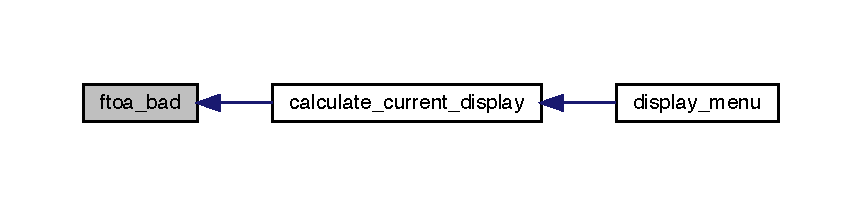
\includegraphics[width=350pt]{vlib_8h_a8805990ed667939e615e4a98950b8bd1_icgraph}
\end{center}
\end{figure}
\mbox{\label{vlib_8h_a08fa7134f8b9a80eeba25f9feab22892}} 
\index{vlib.\+h@{vlib.\+h}!itoa\+\_\+bad@{itoa\+\_\+bad}}
\index{itoa\+\_\+bad@{itoa\+\_\+bad}!vlib.\+h@{vlib.\+h}}
\paragraph{itoa\+\_\+bad()}
{\footnotesize\ttfamily int itoa\+\_\+bad (\begin{DoxyParamCaption}\item[{int}]{a,  }\item[{char $\ast$}]{buffer,  }\item[{int}]{digits }\end{DoxyParamCaption})}



converts a int to string. 


\begin{DoxyParams}{Parameters}
{\em a} & the integer \\
\hline
{\em buffer} & the string the int will be written to. \\
\hline
{\em digits} & the number of digits to be written \\
\hline
\end{DoxyParams}
\begin{DoxyReturn}{Returns}
the digits 
\end{DoxyReturn}
\begin{DoxyAuthor}{Author}
Chris Jerrett, Christian De\+Simone 
\end{DoxyAuthor}
\begin{DoxyDate}{Date}
9/9/2017 
\end{DoxyDate}


Definition at line \textbf{ 13} of file \textbf{ vlib.\+c}.



References \textbf{ reverse()}.



Referenced by \textbf{ calculate\+\_\+current\+\_\+display()}, and \textbf{ ftoa\+\_\+bad()}.


\begin{DoxyCode}
00013                                               \{
00014   \textcolor{keywordtype}{int} i = 0;
00015    \textcolor{keywordflow}{while} (a) \{
00016        buffer[i++] = (a%10) + \textcolor{charliteral}{'0'};
00017        a = a/10;
00018    \}
00019 
00020    \textcolor{comment}{// If number of digits required is more, then}
00021    \textcolor{comment}{// add 0s at the beginning}
00022    \textcolor{keywordflow}{while} (i < digits)
00023        buffer[i++] = \textcolor{charliteral}{'0'};
00024 
00025    reverse(buffer, i);
00026    buffer[i] = \textcolor{charliteral}{'\(\backslash\)0'};
00027    \textcolor{keywordflow}{return} i;
00028 \}
\end{DoxyCode}
Here is the call graph for this function\+:\nopagebreak
\begin{figure}[H]
\begin{center}
\leavevmode
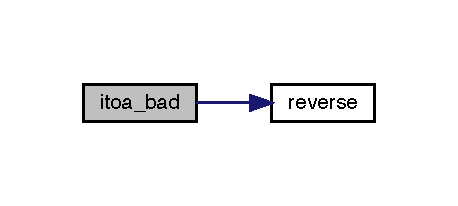
\includegraphics[width=220pt]{vlib_8h_a08fa7134f8b9a80eeba25f9feab22892_cgraph}
\end{center}
\end{figure}
Here is the caller graph for this function\+:\nopagebreak
\begin{figure}[H]
\begin{center}
\leavevmode
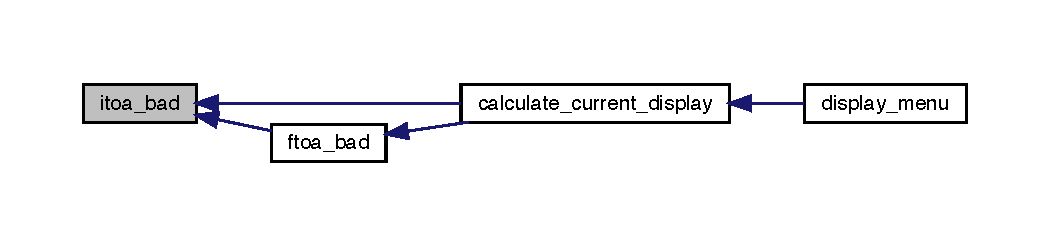
\includegraphics[width=350pt]{vlib_8h_a08fa7134f8b9a80eeba25f9feab22892_icgraph}
\end{center}
\end{figure}
\mbox{\label{vlib_8h_aad7fea725cb4b198ace1aa3df5051244}} 
\index{vlib.\+h@{vlib.\+h}!reverse@{reverse}}
\index{reverse@{reverse}!vlib.\+h@{vlib.\+h}}
\paragraph{reverse()}
{\footnotesize\ttfamily void reverse (\begin{DoxyParamCaption}\item[{char $\ast$}]{str,  }\item[{int}]{len }\end{DoxyParamCaption})}



reverses a string \textquotesingle{}str\textquotesingle{} of length \textquotesingle{}len\textquotesingle{} 

\begin{DoxyAuthor}{Author}
Chris Jerrett 
\end{DoxyAuthor}
\begin{DoxyDate}{Date}
9/9/2017 
\end{DoxyDate}

\begin{DoxyParams}{Parameters}
{\em str} & the string to reverse \\
\hline
{\em len} & the length \\
\hline
\end{DoxyParams}


Definition at line \textbf{ 3} of file \textbf{ vlib.\+c}.



Referenced by \textbf{ itoa\+\_\+bad()}.


\begin{DoxyCode}
00003                                  \{
00004     \textcolor{keywordtype}{int} i=0, j=len-1, temp;
00005     \textcolor{keywordflow}{while} (i<j) \{
00006         temp = str[i];
00007         str[i] = str[j];
00008         str[j] = temp;
00009         i++; j--;
00010     \}
00011 \}
\end{DoxyCode}
Here is the caller graph for this function\+:\nopagebreak
\begin{figure}[H]
\begin{center}
\leavevmode
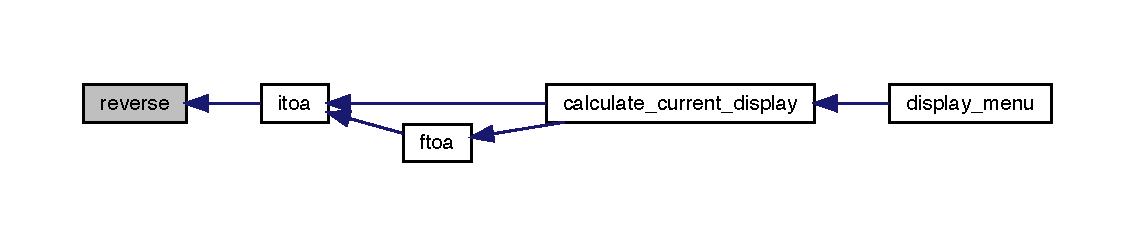
\includegraphics[width=350pt]{vlib_8h_aad7fea725cb4b198ace1aa3df5051244_icgraph}
\end{center}
\end{figure}

\subsection{include/vmath.h File Reference}
\label{vmath_8h}\index{include/vmath.\+h@{include/vmath.\+h}}


Vex Specific Math Functions, includes\+: Cartesian to polar cordinates.  


{\ttfamily \#include $<$math.\+h$>$}\newline
\subsubsection*{Data Structures}
\begin{DoxyCompactItemize}
\item 
struct \textbf{ cord}
\begin{DoxyCompactList}\small\item\em A struct that contains cartesian coordinates. \end{DoxyCompactList}\item 
struct \textbf{ polar\+\_\+cord}
\begin{DoxyCompactList}\small\item\em A struct that contains polar coordinates. \end{DoxyCompactList}\end{DoxyCompactItemize}
\subsubsection*{Macros}
\begin{DoxyCompactItemize}
\item 
\#define \textbf{ M\+\_\+\+PI}~3.\+14159265358979323846
\end{DoxyCompactItemize}
\subsubsection*{Functions}
\begin{DoxyCompactItemize}
\item 
struct \textbf{ polar\+\_\+cord} \textbf{ cartesian\+\_\+cord\+\_\+to\+\_\+polar} (struct \textbf{ cord} cords)
\begin{DoxyCompactList}\small\item\em Function to convert x and y 2 dimensional cartesian cordinated to polar coordinates. \end{DoxyCompactList}\item 
struct \textbf{ polar\+\_\+cord} \textbf{ cartesian\+\_\+to\+\_\+polar} (float x, float y)
\begin{DoxyCompactList}\small\item\em Function to convert x and y 2 dimensional cartesian coordinated to polar coordinates. \end{DoxyCompactList}\item 
int \textbf{ max} (int a, int b)
\begin{DoxyCompactList}\small\item\em the min of two values \end{DoxyCompactList}\item 
int \textbf{ min} (int a, int b)
\begin{DoxyCompactList}\small\item\em the min of two values \end{DoxyCompactList}\item 
double \textbf{ sind} (double angle)
\begin{DoxyCompactList}\small\item\em sine of a angle in degrees \end{DoxyCompactList}\end{DoxyCompactItemize}


\subsubsection{Detailed Description}
Vex Specific Math Functions, includes\+: Cartesian to polar cordinates. 

\begin{DoxyAuthor}{Author}
Christian Desimone 

Chris Jerrett 
\end{DoxyAuthor}
\begin{DoxyDate}{Date}
9/9/2017 
\end{DoxyDate}


Definition in file \textbf{ vmath.\+h}.



\subsubsection{Macro Definition Documentation}
\mbox{\label{vmath_8h_ae71449b1cc6e6250b91f539153a7a0d3}} 
\index{vmath.\+h@{vmath.\+h}!M\+\_\+\+PI@{M\+\_\+\+PI}}
\index{M\+\_\+\+PI@{M\+\_\+\+PI}!vmath.\+h@{vmath.\+h}}
\paragraph{M\+\_\+\+PI}
{\footnotesize\ttfamily \#define M\+\_\+\+PI~3.\+14159265358979323846}



Definition at line \textbf{ 13} of file \textbf{ vmath.\+h}.



Referenced by \textbf{ calculate\+\_\+encoder\+\_\+odemetry()}, and \textbf{ sind()}.



\subsubsection{Function Documentation}
\mbox{\label{vmath_8h_a832105cf858b3046c57c0d08a4e7c38b}} 
\index{vmath.\+h@{vmath.\+h}!cartesian\+\_\+cord\+\_\+to\+\_\+polar@{cartesian\+\_\+cord\+\_\+to\+\_\+polar}}
\index{cartesian\+\_\+cord\+\_\+to\+\_\+polar@{cartesian\+\_\+cord\+\_\+to\+\_\+polar}!vmath.\+h@{vmath.\+h}}
\paragraph{cartesian\+\_\+cord\+\_\+to\+\_\+polar()}
{\footnotesize\ttfamily struct \textbf{ polar\+\_\+cord} cartesian\+\_\+cord\+\_\+to\+\_\+polar (\begin{DoxyParamCaption}\item[{struct \textbf{ cord}}]{cords }\end{DoxyParamCaption})}



Function to convert x and y 2 dimensional cartesian cordinated to polar coordinates. 

\begin{DoxyAuthor}{Author}
Christian Desimone 
\end{DoxyAuthor}
\begin{DoxyDate}{Date}
9/8/2017
\end{DoxyDate}

\begin{DoxyParams}{Parameters}
{\em cords} & the cartesian cords \\
\hline
\end{DoxyParams}
\begin{DoxyReturn}{Returns}
a struct containing the angle and magnitude. 
\end{DoxyReturn}
\begin{DoxySeeAlso}{See also}
\doxyref{polar\+\_\+cord}{p.}{structpolar__cord} 

\doxyref{cord}{p.}{structcord} 
\end{DoxySeeAlso}


Definition at line \textbf{ 53} of file \textbf{ vmath.\+c}.



References \textbf{ cartesian\+\_\+to\+\_\+polar()}.

\mbox{\label{vmath_8h_a1c4a1747b714f5d4654f0614193f9e49}} 
\index{vmath.\+h@{vmath.\+h}!cartesian\+\_\+to\+\_\+polar@{cartesian\+\_\+to\+\_\+polar}}
\index{cartesian\+\_\+to\+\_\+polar@{cartesian\+\_\+to\+\_\+polar}!vmath.\+h@{vmath.\+h}}
\paragraph{cartesian\+\_\+to\+\_\+polar()}
{\footnotesize\ttfamily struct \textbf{ polar\+\_\+cord} cartesian\+\_\+to\+\_\+polar (\begin{DoxyParamCaption}\item[{float}]{x,  }\item[{float}]{y }\end{DoxyParamCaption})}



Function to convert x and y 2 dimensional cartesian coordinated to polar coordinates. 

\begin{DoxyAuthor}{Author}
Christian Desimone 
\end{DoxyAuthor}
\begin{DoxyDate}{Date}
9/8/2017
\end{DoxyDate}

\begin{DoxyParams}{Parameters}
{\em x} & float value of the x cartesian coordinate. \\
\hline
{\em y} & float value of the y cartesian coordinate. \\
\hline
\end{DoxyParams}
\begin{DoxyReturn}{Returns}
a struct containing the angle and magnitude. 
\end{DoxyReturn}
\begin{DoxySeeAlso}{See also}
\doxyref{polar\+\_\+cord}{p.}{structpolar__cord} 
\end{DoxySeeAlso}


Definition at line \textbf{ 15} of file \textbf{ vmath.\+c}.



References \textbf{ polar\+\_\+cord\+::angle}, and \textbf{ polar\+\_\+cord\+::magnitue}.



Referenced by \textbf{ cartesian\+\_\+cord\+\_\+to\+\_\+polar()}.

\mbox{\label{vmath_8h_af082905f7eac6d03e92015146bbc1925}} 
\index{vmath.\+h@{vmath.\+h}!max@{max}}
\index{max@{max}!vmath.\+h@{vmath.\+h}}
\paragraph{max()}
{\footnotesize\ttfamily int max (\begin{DoxyParamCaption}\item[{int}]{a,  }\item[{int}]{b }\end{DoxyParamCaption})}



the min of two values 


\begin{DoxyParams}{Parameters}
{\em a} & the first \\
\hline
{\em b} & the second \\
\hline
\end{DoxyParams}
\begin{DoxyReturn}{Returns}
the smaller of a and b 
\end{DoxyReturn}


Definition at line \textbf{ 83} of file \textbf{ vmath.\+c}.



Referenced by \textbf{ calculate\+\_\+current\+\_\+display()}, \textbf{ init\+\_\+menu\+\_\+float()}, and \textbf{ init\+\_\+menu\+\_\+int()}.

\mbox{\label{vmath_8h_abd8bbcfabb3ddef2ccaafb9928a37b95}} 
\index{vmath.\+h@{vmath.\+h}!min@{min}}
\index{min@{min}!vmath.\+h@{vmath.\+h}}
\paragraph{min()}
{\footnotesize\ttfamily int min (\begin{DoxyParamCaption}\item[{int}]{a,  }\item[{int}]{b }\end{DoxyParamCaption})}



the min of two values 


\begin{DoxyParams}{Parameters}
{\em a} & the first \\
\hline
{\em b} & the second \\
\hline
\end{DoxyParams}
\begin{DoxyReturn}{Returns}
the smaller of a and b 
\end{DoxyReturn}


Definition at line \textbf{ 71} of file \textbf{ vmath.\+c}.



Referenced by \textbf{ calculate\+\_\+current\+\_\+display()}, \textbf{ init\+\_\+menu\+\_\+float()}, and \textbf{ init\+\_\+menu\+\_\+int()}.

\mbox{\label{vmath_8h_a2b83ceb814c90ebfa042a26d884ac159}} 
\index{vmath.\+h@{vmath.\+h}!sind@{sind}}
\index{sind@{sind}!vmath.\+h@{vmath.\+h}}
\paragraph{sind()}
{\footnotesize\ttfamily double sind (\begin{DoxyParamCaption}\item[{double}]{angle }\end{DoxyParamCaption})}



sine of a angle in degrees 



Definition at line \textbf{ 60} of file \textbf{ vmath.\+c}.



References \textbf{ M\+\_\+\+PI}.


\subsection{R\+E\+A\+D\+M\+E.\+md File Reference}
\label{_r_e_a_d_m_e_8md}\index{R\+E\+A\+D\+M\+E.\+md@{R\+E\+A\+D\+M\+E.\+md}}

\hypertarget{auto_8c}{}\section{src/auto.c File Reference}
\label{auto_8c}\index{src/auto.\+c@{src/auto.\+c}}


File for autonomous code.  


{\ttfamily \#include \char`\"{}main.\+h\char`\"{}}\newline
\subsection*{Functions}
\begin{DoxyCompactItemize}
\item 
void \hyperlink{auto_8c_a3c7ca506bbc071fa740de13805b7f376}{autonomous} ()
\end{DoxyCompactItemize}


\subsection{Detailed Description}
File for autonomous code. 

This file should contain the user \hyperlink{auto_8c_a3c7ca506bbc071fa740de13805b7f376}{autonomous()} function and any functions related to it.

Any copyright is dedicated to the Public Domain. \href{http://creativecommons.org/publicdomain/zero/1.0/}{\tt http\+://creativecommons.\+org/publicdomain/zero/1.\+0/}

P\+R\+OS contains Free\+R\+T\+OS (\href{http://www.freertos.org}{\tt http\+://www.\+freertos.\+org}) whose source code may be obtained from \href{http://sourceforge.net/projects/freertos/files/}{\tt http\+://sourceforge.\+net/projects/freertos/files/} or on request. 

\subsection{Function Documentation}
\mbox{\Hypertarget{auto_8c_a3c7ca506bbc071fa740de13805b7f376}\label{auto_8c_a3c7ca506bbc071fa740de13805b7f376}} 
\index{auto.\+c@{auto.\+c}!autonomous@{autonomous}}
\index{autonomous@{autonomous}!auto.\+c@{auto.\+c}}
\subsubsection{\texorpdfstring{autonomous()}{autonomous()}}
{\footnotesize\ttfamily void autonomous (\begin{DoxyParamCaption}{ }\end{DoxyParamCaption})}

Runs the user autonomous code. This function will be started in its own task with the default priority and stack size whenever the robot is enabled via the Field Management System or the V\+EX Competition Switch in the autonomous mode. If the robot is disabled or communications is lost, the autonomous task will be stopped by the kernel. Re-\/enabling the robot will restart the task, not re-\/start it from where it left off.

Code running in the autonomous task cannot access information from the V\+EX Joystick. However, the autonomous function can be invoked from another task if a V\+EX Competition Switch is not available, and it can access joystick information if called in this way.

The autonomous task may exit, unlike \hyperlink{main_8h_ac71a94af413917f27d108e95c4d6f6a7}{operator\+Control()} which should never exit. If it does so, the robot will await a switch to another mode or disable/enable cycle. 
\subsection{src/battery.c File Reference}
\label{battery_8c}\index{src/battery.\+c@{src/battery.\+c}}
{\ttfamily \#include \char`\"{}battery.\+h\char`\"{}}\newline
{\ttfamily \#include $<$A\+P\+I.\+h$>$}\newline
Include dependency graph for battery.\+c\+:\nopagebreak
\begin{figure}[H]
\begin{center}
\leavevmode
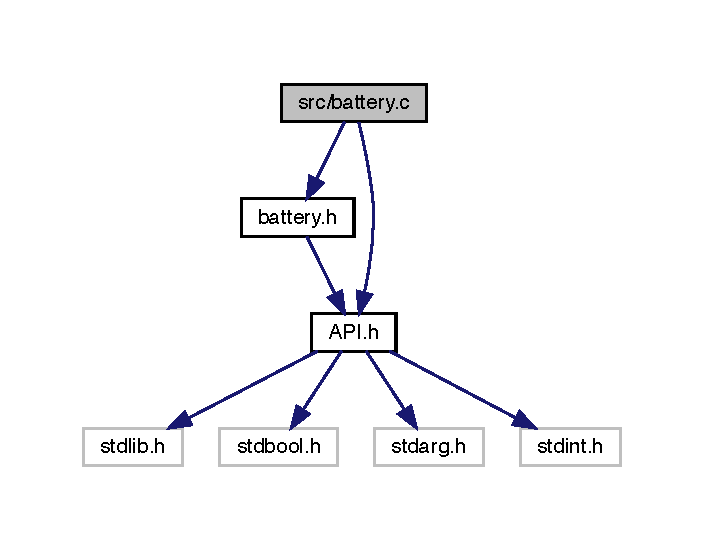
\includegraphics[width=338pt]{battery_8c__incl}
\end{center}
\end{figure}
\subsubsection*{Functions}
\begin{DoxyCompactItemize}
\item 
double \textbf{ backup\+\_\+battery\+\_\+voltage} ()
\begin{DoxyCompactList}\small\item\em gets the backup battery voltage \end{DoxyCompactList}\item 
bool \textbf{ battery\+\_\+level\+\_\+acceptable} ()
\begin{DoxyCompactList}\small\item\em returns if the batteries are acceptable \end{DoxyCompactList}\item 
double \textbf{ main\+\_\+battery\+\_\+voltage} ()
\begin{DoxyCompactList}\small\item\em gets the main battery voltage \end{DoxyCompactList}\end{DoxyCompactItemize}


\subsubsection{Function Documentation}
\mbox{\label{battery_8c_a9b1c5cf7ddddebf63796050a1d4a9969}} 
\index{battery.\+c@{battery.\+c}!backup\+\_\+battery\+\_\+voltage@{backup\+\_\+battery\+\_\+voltage}}
\index{backup\+\_\+battery\+\_\+voltage@{backup\+\_\+battery\+\_\+voltage}!battery.\+c@{battery.\+c}}
\paragraph{backup\+\_\+battery\+\_\+voltage()}
{\footnotesize\ttfamily double backup\+\_\+battery\+\_\+voltage (\begin{DoxyParamCaption}{ }\end{DoxyParamCaption})}



gets the backup battery voltage 

\begin{DoxyAuthor}{Author}
Chris Jerrett 
\end{DoxyAuthor}


Definition at line \textbf{ 17} of file \textbf{ battery.\+c}.



References \textbf{ power\+Level\+Backup()}.



Referenced by \textbf{ battery\+\_\+level\+\_\+acceptable()}.


\begin{DoxyCode}
00017                                 \{
00018   \textcolor{keywordflow}{return} powerLevelBackup() / 1000.0;
00019 \}
\end{DoxyCode}
Here is the call graph for this function\+:\nopagebreak
\begin{figure}[H]
\begin{center}
\leavevmode
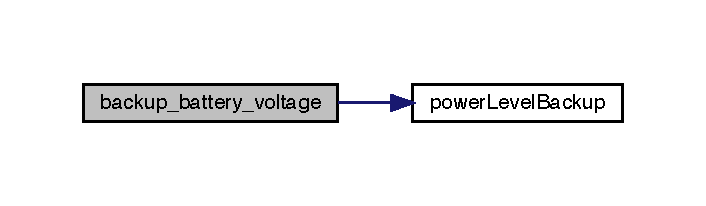
\includegraphics[width=339pt]{battery_8c_a9b1c5cf7ddddebf63796050a1d4a9969_cgraph}
\end{center}
\end{figure}
Here is the caller graph for this function\+:\nopagebreak
\begin{figure}[H]
\begin{center}
\leavevmode
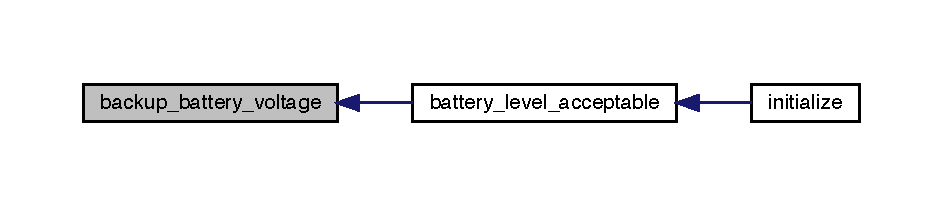
\includegraphics[width=350pt]{battery_8c_a9b1c5cf7ddddebf63796050a1d4a9969_icgraph}
\end{center}
\end{figure}
\mbox{\label{battery_8c_a1097bbb878f6e2690f8eea6cd231959a}} 
\index{battery.\+c@{battery.\+c}!battery\+\_\+level\+\_\+acceptable@{battery\+\_\+level\+\_\+acceptable}}
\index{battery\+\_\+level\+\_\+acceptable@{battery\+\_\+level\+\_\+acceptable}!battery.\+c@{battery.\+c}}
\paragraph{battery\+\_\+level\+\_\+acceptable()}
{\footnotesize\ttfamily bool battery\+\_\+level\+\_\+acceptable (\begin{DoxyParamCaption}{ }\end{DoxyParamCaption})}



returns if the batteries are acceptable 

\begin{DoxySeeAlso}{See also}
\doxyref{M\+I\+N\+\_\+\+M\+A\+I\+N\+\_\+\+V\+O\+L\+T\+A\+GE}{p.}{battery_8h_a63f8a91bb74417aa77dc00340b6fd007} 

\doxyref{M\+I\+N\+\_\+\+B\+A\+C\+K\+U\+P\+\_\+\+V\+O\+L\+T\+A\+GE}{p.}{battery_8h_a0713ec94f47c403bf536ab6b11833b81}
\end{DoxySeeAlso}
\begin{DoxyAuthor}{Author}
Chris Jerrett 
\end{DoxyAuthor}


Definition at line \textbf{ 28} of file \textbf{ battery.\+c}.



References \textbf{ backup\+\_\+battery\+\_\+voltage()}, \textbf{ main\+\_\+battery\+\_\+voltage()}, \textbf{ M\+I\+N\+\_\+\+B\+A\+C\+K\+U\+P\+\_\+\+V\+O\+L\+T\+A\+GE}, and \textbf{ M\+I\+N\+\_\+\+M\+A\+I\+N\+\_\+\+V\+O\+L\+T\+A\+GE}.


\begin{DoxyCode}
00028                                 \{
00029   \textcolor{keywordflow}{if}(main_battery_voltage() < MIN_MAIN_VOLTAGE) \textcolor{keywordflow}{return} \textcolor{keyword}{false};
00030   \textcolor{keywordflow}{if}(backup_battery_voltage() < MIN_BACKUP_VOLTAGE) \textcolor{keywordflow}{return} \textcolor{keyword}{false};
00031   \textcolor{keywordflow}{return} \textcolor{keyword}{true};
00032 \}
\end{DoxyCode}
Here is the call graph for this function\+:\nopagebreak
\begin{figure}[H]
\begin{center}
\leavevmode
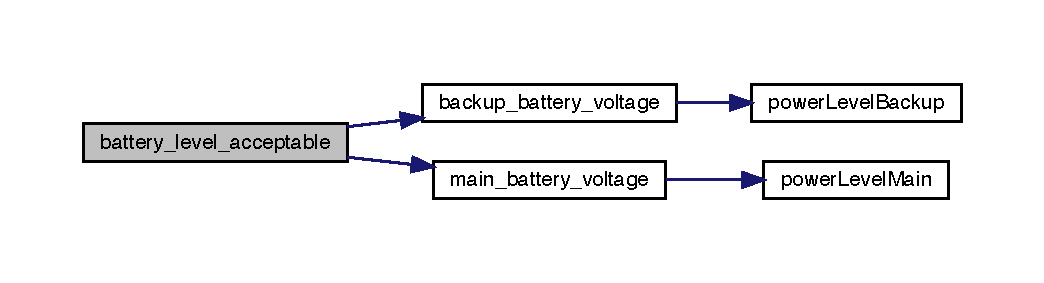
\includegraphics[width=350pt]{battery_8c_a1097bbb878f6e2690f8eea6cd231959a_cgraph}
\end{center}
\end{figure}
\mbox{\label{battery_8c_a8c92c389534fdb079698cdebeb7f2efa}} 
\index{battery.\+c@{battery.\+c}!main\+\_\+battery\+\_\+voltage@{main\+\_\+battery\+\_\+voltage}}
\index{main\+\_\+battery\+\_\+voltage@{main\+\_\+battery\+\_\+voltage}!battery.\+c@{battery.\+c}}
\paragraph{main\+\_\+battery\+\_\+voltage()}
{\footnotesize\ttfamily double main\+\_\+battery\+\_\+voltage (\begin{DoxyParamCaption}{ }\end{DoxyParamCaption})}



gets the main battery voltage 

\begin{DoxyAuthor}{Author}
Chris Jerrett 
\end{DoxyAuthor}


Definition at line \textbf{ 9} of file \textbf{ battery.\+c}.



References \textbf{ power\+Level\+Main()}.



Referenced by \textbf{ battery\+\_\+level\+\_\+acceptable()}.


\begin{DoxyCode}
00009                               \{
00010   \textcolor{keywordflow}{return} powerLevelMain() / 1000.0;
00011 \}
\end{DoxyCode}
Here is the call graph for this function\+:\nopagebreak
\begin{figure}[H]
\begin{center}
\leavevmode
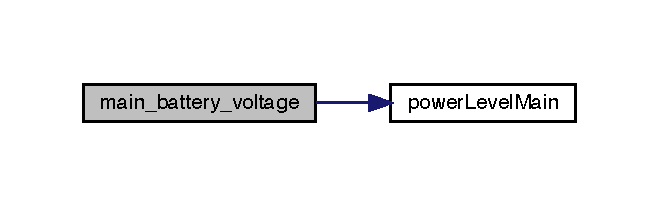
\includegraphics[width=316pt]{battery_8c_a8c92c389534fdb079698cdebeb7f2efa_cgraph}
\end{center}
\end{figure}
Here is the caller graph for this function\+:\nopagebreak
\begin{figure}[H]
\begin{center}
\leavevmode
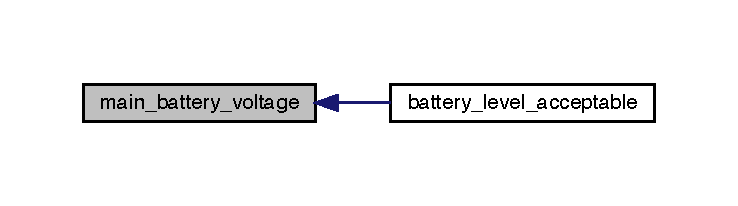
\includegraphics[width=350pt]{battery_8c_a8c92c389534fdb079698cdebeb7f2efa_icgraph}
\end{center}
\end{figure}

\hypertarget{controller_8c}{}\section{src/controller.c File Reference}
\label{controller_8c}\index{src/controller.\+c@{src/controller.\+c}}
{\ttfamily \#include \char`\"{}controller.\+h\char`\"{}}\newline
Include dependency graph for controller.\+c\+:\nopagebreak
\begin{figure}[H]
\begin{center}
\leavevmode
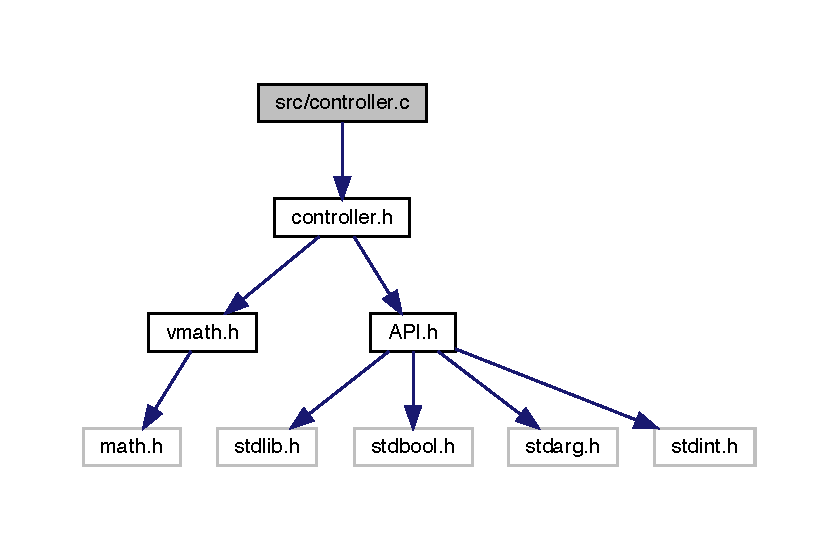
\includegraphics[width=350pt]{controller_8c__incl}
\end{center}
\end{figure}
\subsection*{Functions}
\begin{DoxyCompactItemize}
\item 
struct \hyperlink{structcord}{cord} \hyperlink{controller_8c_a0ce0176099c0bb15ad8c36123222059d}{get\+\_\+joystick\+\_\+cord} (enum \hyperlink{controller_8h_ac365c9e892abe4a1b85ae8f56a4eae5a}{joystick} \hyperlink{drive_8h_afc015eff6557e84151d2e53b94375445}{side}, int controller)
\begin{DoxyCompactList}\small\item\em Gets the location of a joystick on the controller. \end{DoxyCompactList}\end{DoxyCompactItemize}


\subsection{Function Documentation}
\mbox{\Hypertarget{controller_8c_a0ce0176099c0bb15ad8c36123222059d}\label{controller_8c_a0ce0176099c0bb15ad8c36123222059d}} 
\index{controller.\+c@{controller.\+c}!get\+\_\+joystick\+\_\+cord@{get\+\_\+joystick\+\_\+cord}}
\index{get\+\_\+joystick\+\_\+cord@{get\+\_\+joystick\+\_\+cord}!controller.\+c@{controller.\+c}}
\subsubsection{\texorpdfstring{get\+\_\+joystick\+\_\+cord()}{get\_joystick\_cord()}}
{\footnotesize\ttfamily struct \hyperlink{structcord}{cord} get\+\_\+joystick\+\_\+cord (\begin{DoxyParamCaption}\item[{enum \hyperlink{controller_8h_ac365c9e892abe4a1b85ae8f56a4eae5a}{joystick}}]{side,  }\item[{int}]{controller }\end{DoxyParamCaption})}



Gets the location of a joystick on the controller. 

\begin{DoxyAuthor}{Author}
Chris Jerrett 
\end{DoxyAuthor}


Definition at line 3 of file controller.\+c.



References joystick\+Get\+Analog(), L\+E\+F\+T\+\_\+\+J\+O\+Y\+\_\+X, L\+E\+F\+T\+\_\+\+J\+O\+Y\+\_\+Y, R\+I\+G\+H\+T\+\_\+\+J\+OY, R\+I\+G\+H\+T\+\_\+\+J\+O\+Y\+\_\+X, R\+I\+G\+H\+T\+\_\+\+J\+O\+Y\+\_\+Y, cord\+::x, and cord\+::y.


\begin{DoxyCode}
3                                                                   \{
4   \textcolor{keywordtype}{int} x;
5   \textcolor{keywordtype}{int} y;
6   \textcolor{keywordflow}{if}(\hyperlink{drive_8h_afc015eff6557e84151d2e53b94375445}{side} == \hyperlink{controller_8h_ac365c9e892abe4a1b85ae8f56a4eae5aae08a2d362c677f96f72d93047513cafe}{RIGHT\_JOY}) \{
7     y = \hyperlink{_a_p_i_8h_ad56fcec15d1a48deb8780bb0fc38be4d}{joystickGetAnalog}(controller, \hyperlink{controller_8h_ad74f84aad465437cc1e0f914dbd6fab5}{RIGHT\_JOY\_X});
8     x = \hyperlink{_a_p_i_8h_ad56fcec15d1a48deb8780bb0fc38be4d}{joystickGetAnalog}(controller, \hyperlink{controller_8h_a99457bf9dee795334411ea77f0858b16}{RIGHT\_JOY\_Y});
9   \} \textcolor{keywordflow}{else} \{
10     y = \hyperlink{_a_p_i_8h_ad56fcec15d1a48deb8780bb0fc38be4d}{joystickGetAnalog}(controller, \hyperlink{controller_8h_ac055a23829dc64aa20b8e2e1bcfbf316}{LEFT\_JOY\_X});
11     x = \hyperlink{_a_p_i_8h_ad56fcec15d1a48deb8780bb0fc38be4d}{joystickGetAnalog}(controller, \hyperlink{controller_8h_ae0a2b64db5fc4f4bf4b169185be93db3}{LEFT\_JOY\_Y});
12   \}
13   \textcolor{keyword}{struct }\hyperlink{structcord}{cord} c;
14   c.\hyperlink{structcord_a2eef9b681474b679cf87b0c20eced2cd}{x} = \hyperlink{structcord_a2eef9b681474b679cf87b0c20eced2cd}{x};
15   c.y = \hyperlink{structcord_a4e7d289c55cfe511532e53a81dc19215}{y};
16   \textcolor{keywordflow}{return} c;
17 \}
\end{DoxyCode}
Here is the call graph for this function\+:\nopagebreak
\begin{figure}[H]
\begin{center}
\leavevmode
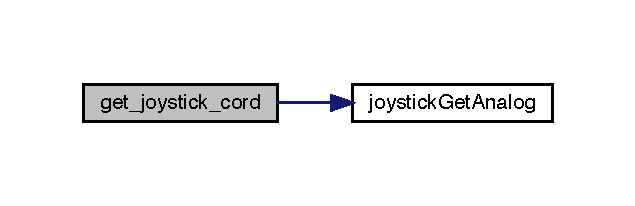
\includegraphics[width=305pt]{controller_8c_a0ce0176099c0bb15ad8c36123222059d_cgraph}
\end{center}
\end{figure}

\subsection{src/drive.c File Reference}
\label{drive_8c}\index{src/drive.\+c@{src/drive.\+c}}
\subsubsection*{Functions}
\begin{DoxyCompactItemize}
\item 
int \textbf{ get\+Thresh} ()
\begin{DoxyCompactList}\small\item\em Gets the deadzone threshhold on the joystick. \end{DoxyCompactList}\item 
static float \textbf{ joystick\+Exp} (int joystick\+Val)
\begin{DoxyCompactList}\small\item\em Applies exponential scale to a joystick value. \end{DoxyCompactList}\item 
void \textbf{ set\+\_\+side\+\_\+speed} (\textbf{ side\+\_\+t} \textbf{ side}, int speed)
\begin{DoxyCompactList}\small\item\em sets the speed of one side of the robot. \end{DoxyCompactList}\item 
void \textbf{ set\+Thresh} (int t)
\begin{DoxyCompactList}\small\item\em Sets the deadzone threshhold on the joystick. \end{DoxyCompactList}\item 
void \textbf{ update\+\_\+drive\+\_\+motors} ()
\begin{DoxyCompactList}\small\item\em Updates the drive motors during teleop. \end{DoxyCompactList}\end{DoxyCompactItemize}
\subsubsection*{Variables}
\begin{DoxyCompactItemize}
\item 
static int \textbf{ thresh} = 10
\end{DoxyCompactItemize}


\subsubsection{Function Documentation}
\mbox{\label{drive_8c_a9caa5e772598f9182c9ec84cf8c351ee}} 
\index{drive.\+c@{drive.\+c}!get\+Thresh@{get\+Thresh}}
\index{get\+Thresh@{get\+Thresh}!drive.\+c@{drive.\+c}}
\paragraph{get\+Thresh()}
{\footnotesize\ttfamily int get\+Thresh (\begin{DoxyParamCaption}{ }\end{DoxyParamCaption})}



Gets the deadzone threshhold on the joystick. 

\begin{DoxyAuthor}{Author}
Christian Desimone 
\end{DoxyAuthor}


Definition at line \textbf{ 12} of file \textbf{ drive.\+c}.



References \textbf{ thresh}.


\begin{DoxyCode}
00012 \{ \textcolor{keywordflow}{return} thresh; \}
\end{DoxyCode}
\mbox{\label{drive_8c_a6de4fbb9197f2f350c53a9f8bf23a8f1}} 
\index{drive.\+c@{drive.\+c}!joystick\+Exp@{joystick\+Exp}}
\index{joystick\+Exp@{joystick\+Exp}!drive.\+c@{drive.\+c}}
\paragraph{joystick\+Exp()}
{\footnotesize\ttfamily static float joystick\+Exp (\begin{DoxyParamCaption}\item[{int}]{joystick\+Val }\end{DoxyParamCaption})\hspace{0.3cm}{\ttfamily [static]}}



Applies exponential scale to a joystick value. 

\begin{DoxyAuthor}{Author}
Christian De\+Simone, Chris Jerrett 
\end{DoxyAuthor}

\begin{DoxyParams}{Parameters}
{\em joystick\+Val} & the analog value from the joystick \\
\hline
\end{DoxyParams}
\begin{DoxyDate}{Date}
9/21/2017 
\end{DoxyDate}


Definition at line \textbf{ 73} of file \textbf{ drive.\+c}.



References \textbf{ thresh}.


\begin{DoxyCode}
00073                                           \{
00074   \textcolor{comment}{// make the offset negative if moving backwards}
00075   \textcolor{keywordflow}{if} (abs(joystickVal) < thresh) \{
00076     \textcolor{keywordflow}{return} 0;
00077   \}
00078 
00079   \textcolor{keywordtype}{int} offset;
00080   \textcolor{comment}{// Use the threshold to ensure the joystick values are significant}
00081   \textcolor{keywordflow}{if} (joystickVal < 0) \{
00082     offset = -(thresh);
00083   \} \textcolor{keywordflow}{else} \{
00084     offset = thresh;
00085   \}
00086   \textcolor{comment}{// Apply the function ((((x/10)^3)/18) + offset) * 0.8 to the joystick value}
00087   \textcolor{keywordflow}{return} (pow(joystickVal / 10, 3) / 18 + offset) * 0.8;
00088 \}
\end{DoxyCode}
\mbox{\label{drive_8c_a8df41fd50094c065eedc81fc5e6595d1}} 
\index{drive.\+c@{drive.\+c}!set\+\_\+side\+\_\+speed@{set\+\_\+side\+\_\+speed}}
\index{set\+\_\+side\+\_\+speed@{set\+\_\+side\+\_\+speed}!drive.\+c@{drive.\+c}}
\paragraph{set\+\_\+side\+\_\+speed()}
{\footnotesize\ttfamily void set\+\_\+side\+\_\+speed (\begin{DoxyParamCaption}\item[{\textbf{ side\+\_\+t}}]{side,  }\item[{int}]{speed }\end{DoxyParamCaption})}



sets the speed of one side of the robot. 

\begin{DoxyAuthor}{Author}
Christian Desimone 
\end{DoxyAuthor}

\begin{DoxyParams}{Parameters}
{\em side} & a side enum which indicates the size. \\
\hline
{\em speed} & the speed of the side. Can range from -\/127 -\/ 127 negative being back and positive forwards \\
\hline
\end{DoxyParams}


Definition at line \textbf{ 54} of file \textbf{ drive.\+c}.



References \textbf{ B\+O\+TH}, \textbf{ L\+E\+FT}, \textbf{ R\+I\+G\+HT}, and \textbf{ set\+\_\+motor\+\_\+slew()}.



Referenced by \textbf{ auton\+\_\+drive\+\_\+towards\+\_\+mobile\+\_\+goal()}, \textbf{ auton\+\_\+turn\+\_\+180()}, \textbf{ autonomous()}, and \textbf{ update\+\_\+drive\+\_\+motors()}.


\begin{DoxyCode}
00054                                             \{
00055   \textcolor{keywordflow}{if} (side == RIGHT || side == BOTH) \{
00056     set_motor_slew(MOTOR\_BACK\_RIGHT, -speed);
00057     set_motor_slew(MOTOR\_FRONT\_RIGHT, -speed);
00058     set_motor_slew(MOTOR\_MIDDLE\_RIGHT, -speed);
00059   \}
00060   \textcolor{keywordflow}{if} (side == LEFT || side == BOTH) \{
00061     set_motor_slew(MOTOR\_BACK\_LEFT, speed);
00062     set_motor_slew(MOTOR\_MIDDLE\_LEFT, speed);
00063     set_motor_slew(MOTOR\_FRONT\_LEFT, speed);
00064   \}
00065 \}
\end{DoxyCode}
Here is the call graph for this function\+:
\nopagebreak
\begin{figure}[H]
\begin{center}
\leavevmode
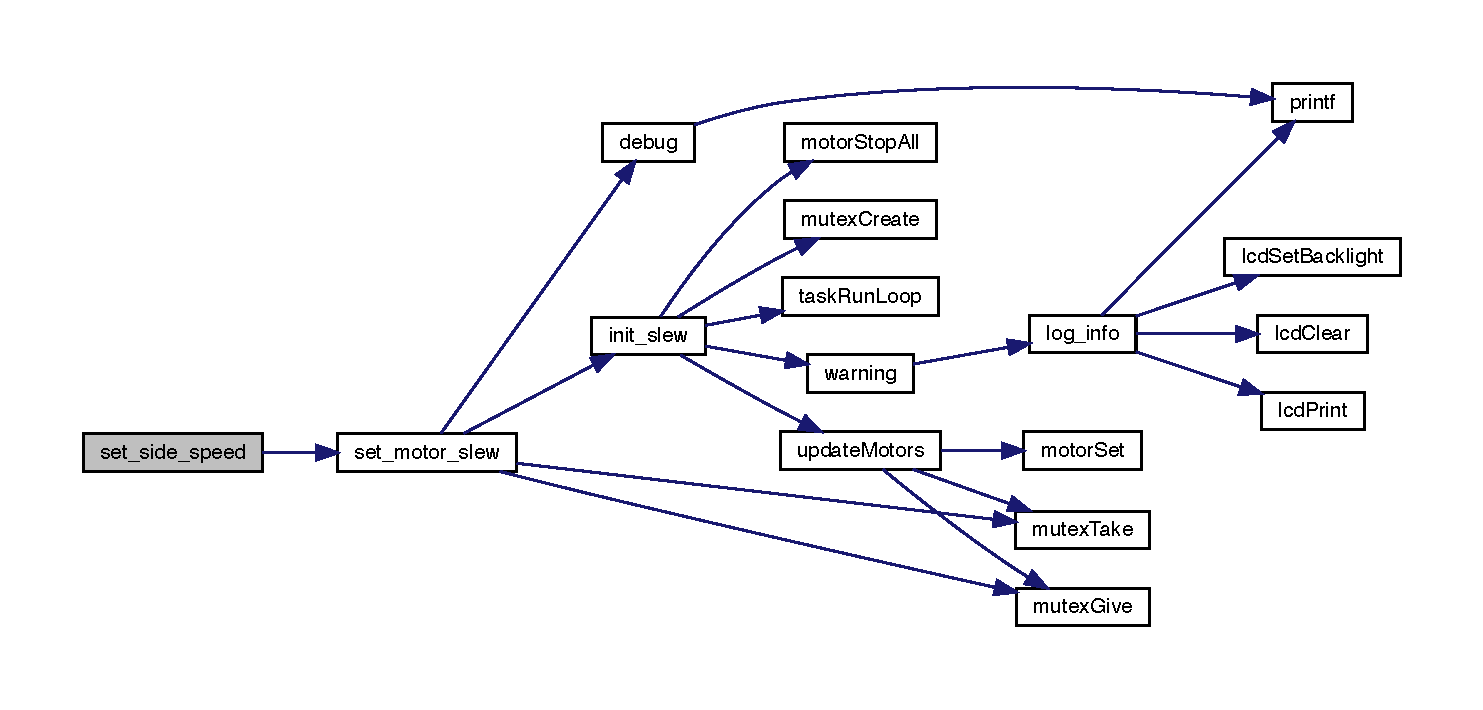
\includegraphics[width=350pt]{drive_8c_a8df41fd50094c065eedc81fc5e6595d1_cgraph}
\end{center}
\end{figure}
Here is the caller graph for this function\+:
\nopagebreak
\begin{figure}[H]
\begin{center}
\leavevmode
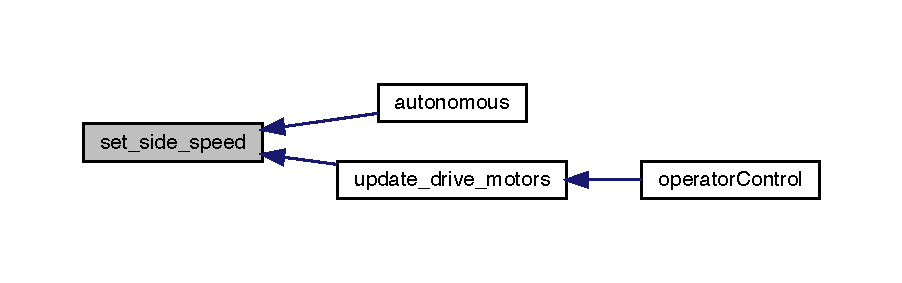
\includegraphics[width=350pt]{drive_8c_a8df41fd50094c065eedc81fc5e6595d1_icgraph}
\end{center}
\end{figure}
\mbox{\label{drive_8c_a53d6e35d53ec3e0b1b1c489d8203f204}} 
\index{drive.\+c@{drive.\+c}!set\+Thresh@{set\+Thresh}}
\index{set\+Thresh@{set\+Thresh}!drive.\+c@{drive.\+c}}
\paragraph{set\+Thresh()}
{\footnotesize\ttfamily void set\+Thresh (\begin{DoxyParamCaption}\item[{int}]{t }\end{DoxyParamCaption})}



Sets the deadzone threshhold on the joystick. 

Sets the deadzone threshhold on the drive.

\begin{DoxyAuthor}{Author}
Christian Desimone 
\end{DoxyAuthor}


Definition at line \textbf{ 18} of file \textbf{ drive.\+c}.



References \textbf{ thresh}.


\begin{DoxyCode}
00018 \{ thresh = t; \}
\end{DoxyCode}
\mbox{\label{drive_8c_a8224a4626a934d30ed587671b7004bf8}} 
\index{drive.\+c@{drive.\+c}!update\+\_\+drive\+\_\+motors@{update\+\_\+drive\+\_\+motors}}
\index{update\+\_\+drive\+\_\+motors@{update\+\_\+drive\+\_\+motors}!drive.\+c@{drive.\+c}}
\paragraph{update\+\_\+drive\+\_\+motors()}
{\footnotesize\ttfamily void update\+\_\+drive\+\_\+motors (\begin{DoxyParamCaption}{ }\end{DoxyParamCaption})}



Updates the drive motors during teleop. 

\begin{DoxyAuthor}{Author}
Christian Desimone 
\end{DoxyAuthor}
\begin{DoxyDate}{Date}
9/5/17 
\end{DoxyDate}


Definition at line \textbf{ 25} of file \textbf{ drive.\+c}.



References \textbf{ joystick\+Get\+Analog()}, \textbf{ L\+E\+FT}, \textbf{ R\+I\+G\+HT}, \textbf{ set\+\_\+side\+\_\+speed()}, \textbf{ thresh}, \textbf{ cord\+::x}, and \textbf{ cord\+::y}.



Referenced by \textbf{ operator\+Control()}.


\begin{DoxyCode}
00025                            \{
00026   \textcolor{comment}{// Get the joystick values from the controller}
00027   \textcolor{keywordtype}{int} x = 0;
00028   \textcolor{keywordtype}{int} y = 0;
00029   x = -(joystickGetAnalog(MASTER, 3));
00030   y = (joystickGetAnalog(MASTER, 1));
00031   \textcolor{comment}{// Make sure the joystick values are significant enough to change the motors}
00032   \textcolor{keywordflow}{if} (x < thresh && x > -thresh) \{
00033     x = 0;
00034   \}
00035   \textcolor{keywordflow}{if} (y < thresh && y > -thresh) \{
00036     y = 0;
00037   \}
00038   \textcolor{comment}{// Create motor values for the left and right from the x and y of the joystick}
00039   \textcolor{keywordtype}{int} r = (x + y);
00040   \textcolor{keywordtype}{int} l = -(x - y);
00041 
00042   \textcolor{comment}{// Set the drive motors}
00043   set_side_speed(LEFT, l);
00044   set_side_speed(RIGHT, -r);
00045 \}
\end{DoxyCode}
Here is the call graph for this function\+:
\nopagebreak
\begin{figure}[H]
\begin{center}
\leavevmode
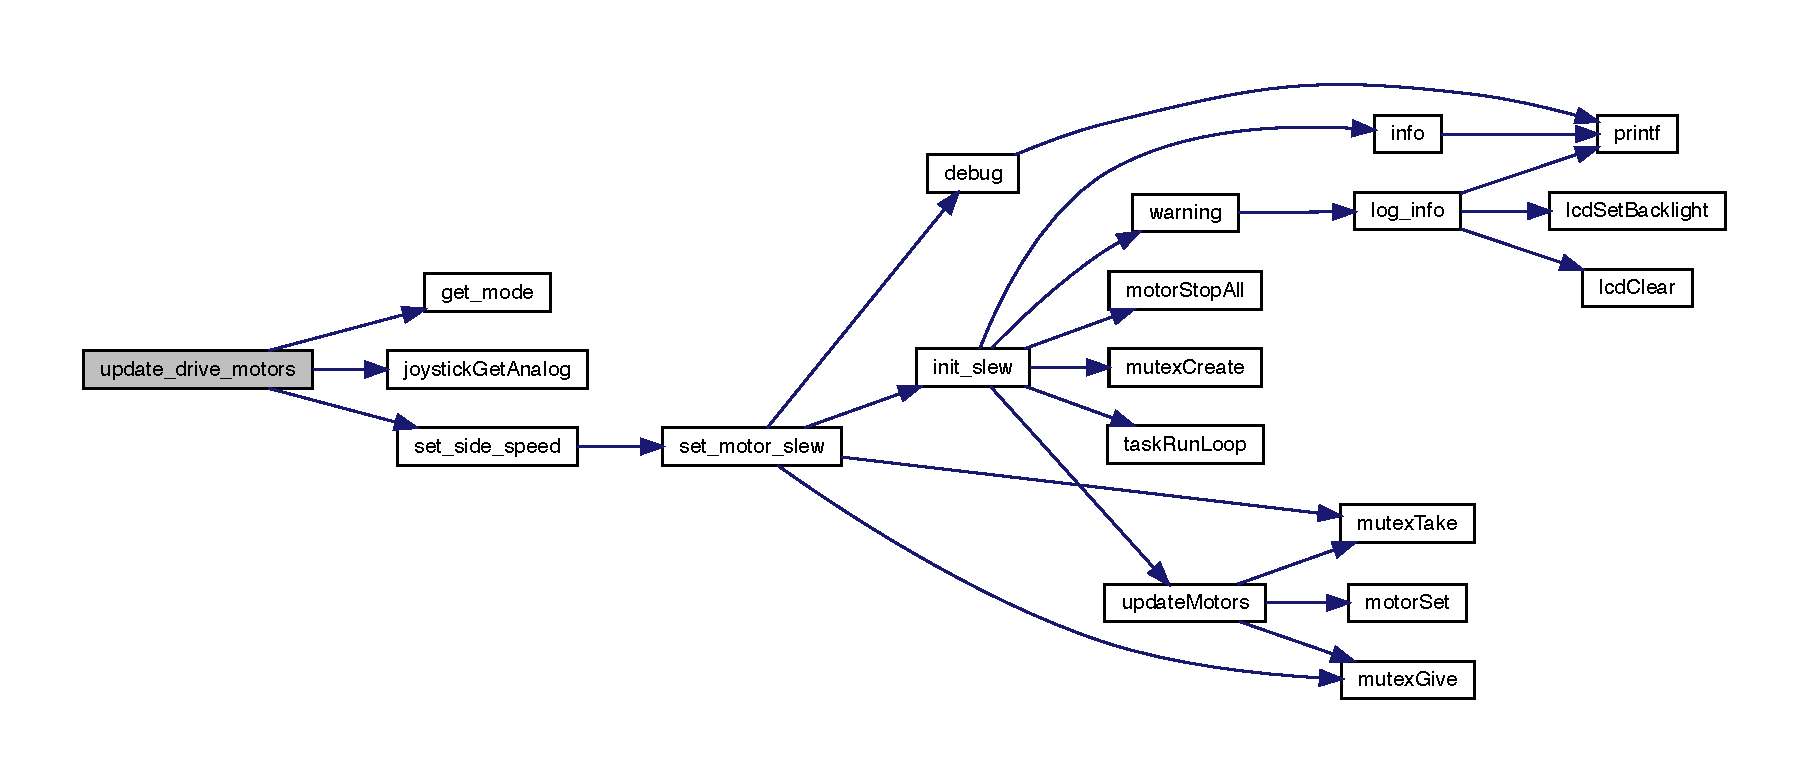
\includegraphics[width=350pt]{drive_8c_a8224a4626a934d30ed587671b7004bf8_cgraph}
\end{center}
\end{figure}
Here is the caller graph for this function\+:
\nopagebreak
\begin{figure}[H]
\begin{center}
\leavevmode
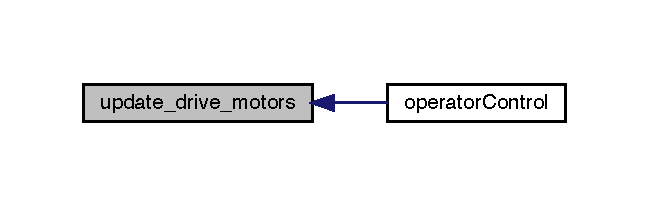
\includegraphics[width=311pt]{drive_8c_a8224a4626a934d30ed587671b7004bf8_icgraph}
\end{center}
\end{figure}


\subsubsection{Variable Documentation}
\mbox{\label{drive_8c_a6cf8bf160a02413bc3d5d18b0294b581}} 
\index{drive.\+c@{drive.\+c}!thresh@{thresh}}
\index{thresh@{thresh}!drive.\+c@{drive.\+c}}
\paragraph{thresh}
{\footnotesize\ttfamily int thresh = 10\hspace{0.3cm}{\ttfamily [static]}}



Definition at line \textbf{ 6} of file \textbf{ drive.\+c}.



Referenced by \textbf{ get\+Thresh()}, \textbf{ joystick\+Exp()}, \textbf{ set\+Thresh()}, and \textbf{ update\+\_\+drive\+\_\+motors()}.


\hypertarget{encoders_8c}{}\section{src/encoders.c File Reference}
\label{encoders_8c}\index{src/encoders.\+c@{src/encoders.\+c}}
{\ttfamily \#include \char`\"{}encoders.\+h\char`\"{}}\newline
{\ttfamily \#include $<$A\+P\+I.\+h$>$}\newline
Include dependency graph for encoders.\+c\+:
\nopagebreak
\begin{figure}[H]
\begin{center}
\leavevmode
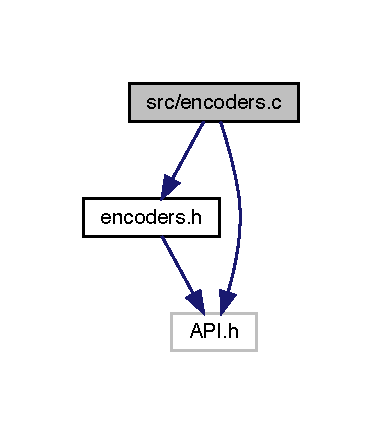
\includegraphics[width=183pt]{encoders_8c__incl}
\end{center}
\end{figure}
\subsection*{Functions}
\begin{DoxyCompactItemize}
\item 
int \hyperlink{encoders_8c_aed261dd4dae33a48c42f2e363c84760f}{get\+\_\+encoder\+\_\+ticks} (unsigned char address)
\begin{DoxyCompactList}\small\item\em Gets the encoder ticks since last reset. \end{DoxyCompactList}\item 
int \hyperlink{encoders_8c_a8e6b77703c5cf18e00709b052fb4bf22}{get\+\_\+encoder\+\_\+velocity} (unsigned char address)
\begin{DoxyCompactList}\small\item\em Gets the encoder reads. \end{DoxyCompactList}\item 
bool \hyperlink{encoders_8c_aa6ec1ca17e907babd52803ecba451cd3}{init\+\_\+encoders} ()
\begin{DoxyCompactList}\small\item\em Initializes all motor encoders. \end{DoxyCompactList}\end{DoxyCompactItemize}


\subsection{Function Documentation}
\mbox{\Hypertarget{encoders_8c_aed261dd4dae33a48c42f2e363c84760f}\label{encoders_8c_aed261dd4dae33a48c42f2e363c84760f}} 
\index{encoders.\+c@{encoders.\+c}!get\+\_\+encoder\+\_\+ticks@{get\+\_\+encoder\+\_\+ticks}}
\index{get\+\_\+encoder\+\_\+ticks@{get\+\_\+encoder\+\_\+ticks}!encoders.\+c@{encoders.\+c}}
\subsubsection{\texorpdfstring{get\+\_\+encoder\+\_\+ticks()}{get\_encoder\_ticks()}}
{\footnotesize\ttfamily int get\+\_\+encoder\+\_\+ticks (\begin{DoxyParamCaption}\item[{unsigned char}]{address }\end{DoxyParamCaption})}



Gets the encoder ticks since last reset. 

\begin{DoxyAuthor}{Author}
Chris Jerrett 
\end{DoxyAuthor}
\begin{DoxyDate}{Date}
9/15/2017 
\end{DoxyDate}


Definition at line 12 of file encoders.\+c.


\begin{DoxyCode}
12                                              \{
13   \textcolor{keywordtype}{int} i = 0;
14   imeGet(address, &i);
15   \textcolor{keywordflow}{return} i;
16 \}
\end{DoxyCode}
\mbox{\Hypertarget{encoders_8c_a8e6b77703c5cf18e00709b052fb4bf22}\label{encoders_8c_a8e6b77703c5cf18e00709b052fb4bf22}} 
\index{encoders.\+c@{encoders.\+c}!get\+\_\+encoder\+\_\+velocity@{get\+\_\+encoder\+\_\+velocity}}
\index{get\+\_\+encoder\+\_\+velocity@{get\+\_\+encoder\+\_\+velocity}!encoders.\+c@{encoders.\+c}}
\subsubsection{\texorpdfstring{get\+\_\+encoder\+\_\+velocity()}{get\_encoder\_velocity()}}
{\footnotesize\ttfamily int get\+\_\+encoder\+\_\+velocity (\begin{DoxyParamCaption}\item[{unsigned char}]{address }\end{DoxyParamCaption})}



Gets the encoder reads. 

\begin{DoxyAuthor}{Author}
Chris Jerrett 
\end{DoxyAuthor}
\begin{DoxyDate}{Date}
9/15/2017 
\end{DoxyDate}


Definition at line 18 of file encoders.\+c.


\begin{DoxyCode}
18                                                 \{
19   \textcolor{keywordtype}{int} i = 0;
20   imeGetVelocity(address, &i);
21   \textcolor{keywordflow}{return} i;
22 \}
\end{DoxyCode}
\mbox{\Hypertarget{encoders_8c_aa6ec1ca17e907babd52803ecba451cd3}\label{encoders_8c_aa6ec1ca17e907babd52803ecba451cd3}} 
\index{encoders.\+c@{encoders.\+c}!init\+\_\+encoders@{init\+\_\+encoders}}
\index{init\+\_\+encoders@{init\+\_\+encoders}!encoders.\+c@{encoders.\+c}}
\subsubsection{\texorpdfstring{init\+\_\+encoders()}{init\_encoders()}}
{\footnotesize\ttfamily bool init\+\_\+encoders (\begin{DoxyParamCaption}{ }\end{DoxyParamCaption})}



Initializes all motor encoders. 

\begin{DoxyAuthor}{Author}
Chris Jerrett 
\end{DoxyAuthor}
\begin{DoxyDate}{Date}
9/9/2017 
\end{DoxyDate}
\begin{DoxySeeAlso}{See also}
\hyperlink{encoders_8h_a87db35d2735ef045f57d446b3bfe8d48}{I\+M\+E\+\_\+\+N\+U\+M\+B\+ER} 
\end{DoxySeeAlso}


Definition at line 4 of file encoders.\+c.



References I\+M\+E\+\_\+\+N\+U\+M\+B\+ER.



Referenced by initialize().


\begin{DoxyCode}
4                      \{
5 \textcolor{preprocessor}{  #ifdef IME\_NUMBER}
6   \textcolor{keywordflow}{return} imeInitializeAll() == \hyperlink{encoders_8h_a87db35d2735ef045f57d446b3bfe8d48}{IME\_NUMBER};
7 \textcolor{preprocessor}{  #else}
8   \textcolor{keywordflow}{return} imeInitializeAll();
9 \textcolor{preprocessor}{  #endif}
10 \}
\end{DoxyCode}
Here is the caller graph for this function\+:
\nopagebreak
\begin{figure}[H]
\begin{center}
\leavevmode
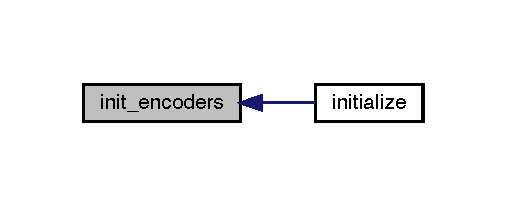
\includegraphics[width=243pt]{encoders_8c_aa6ec1ca17e907babd52803ecba451cd3_icgraph}
\end{center}
\end{figure}

\subsection{src/init.c File Reference}
\label{init_8c}\index{src/init.\+c@{src/init.\+c}}


File for initialization code.  


\subsubsection*{Functions}
\begin{DoxyCompactItemize}
\item 
void \textbf{ initialize} ()
\begin{DoxyCompactList}\small\item\em Runs user initialization code. \end{DoxyCompactList}\item 
void \textbf{ initialize\+IO} ()
\begin{DoxyCompactList}\small\item\em Runs pre-\/initialization code. \end{DoxyCompactList}\end{DoxyCompactItemize}
\subsubsection*{Variables}
\begin{DoxyCompactItemize}
\item 
\textbf{ Ultrasonic} \textbf{ lifter\+\_\+ultrasonic}
\end{DoxyCompactItemize}


\subsubsection{Detailed Description}
File for initialization code. 

This file should contain the user \doxyref{initialize()}{p.}{init_8c_a25a40b6614565f755233080a384c35f1} function and any functions related to it.

Any copyright is dedicated to the Public Domain. {\tt http\+://creativecommons.\+org/publicdomain/zero/1.\+0/}

P\+R\+OS contains Free\+R\+T\+OS ({\tt http\+://www.\+freertos.\+org}) whose source code may be obtained from {\tt http\+://sourceforge.\+net/projects/freertos/files/} or on request. 

Definition in file \textbf{ init.\+c}.



\subsubsection{Function Documentation}
\mbox{\label{init_8c_a25a40b6614565f755233080a384c35f1}} 
\index{init.\+c@{init.\+c}!initialize@{initialize}}
\index{initialize@{initialize}!init.\+c@{init.\+c}}
\paragraph{initialize()}
{\footnotesize\ttfamily void initialize (\begin{DoxyParamCaption}{ }\end{DoxyParamCaption})}



Runs user initialization code. 

This function will be started in its own task with the default priority and stack size once when the robot is starting up. It is possible that the V\+E\+Xnet communication link may not be fully established at this time, so reading from the V\+EX Joystick may fail.

This function should initialize most sensors (gyro, encoders, ultrasonics), L\+C\+Ds, global variables, and I\+M\+Es.

This function must exit relatively promptly, or the \doxyref{operator\+Control()}{p.}{main_8h_ac71a94af413917f27d108e95c4d6f6a7} and \doxyref{autonomous()}{p.}{main_8h_a3c7ca506bbc071fa740de13805b7f376} tasks will not start. An autonomous mode selection menu like the pre\+\_\+auton() in other environments can be implemented in this task if desired. 

Definition at line \textbf{ 52} of file \textbf{ init.\+c}.



References \textbf{ battery\+\_\+level\+\_\+acceptable()}, \textbf{ error()}, \textbf{ info()}, \textbf{ init\+\_\+encoders()}, \textbf{ init\+\_\+error()}, \textbf{ init\+\_\+main\+\_\+lcd()}, \textbf{ init\+\_\+menu\+\_\+var()}, \textbf{ lifter\+\_\+ultrasonic}, \textbf{ set\+Team\+Name()}, \textbf{ S\+T\+R\+I\+N\+G\+\_\+\+T\+Y\+PE}, and \textbf{ ultrasonic\+Init()}.


\begin{DoxyCode}
00052                   \{
00053   init_main_lcd(uart1);
00054   info(\textcolor{stringliteral}{"LCD Init"});
00055   \textcolor{keywordflow}{if} (!battery_level_acceptable())
00056     error(\textcolor{stringliteral}{"Bad main/backup bat"});
00057   menu_t *t =
00058       init_menu_var(STRING_TYPE, \textcolor{stringliteral}{"TEST Menu"}, 5, \textcolor{stringliteral}{"1"}, \textcolor{stringliteral}{"2"}, \textcolor{stringliteral}{"3"}, \textcolor{stringliteral}{"4"}, \textcolor{stringliteral}{"5"});
00059   init_error(\textcolor{keyword}{true}, uart2);
00060   setTeamName(\textcolor{stringliteral}{"9228A"});
00061   init_encoders();
00062   lifter_ultrasonic = ultrasonicInit(4, 5);
00063 \}
\end{DoxyCode}
Here is the call graph for this function\+:
\nopagebreak
\begin{figure}[H]
\begin{center}
\leavevmode
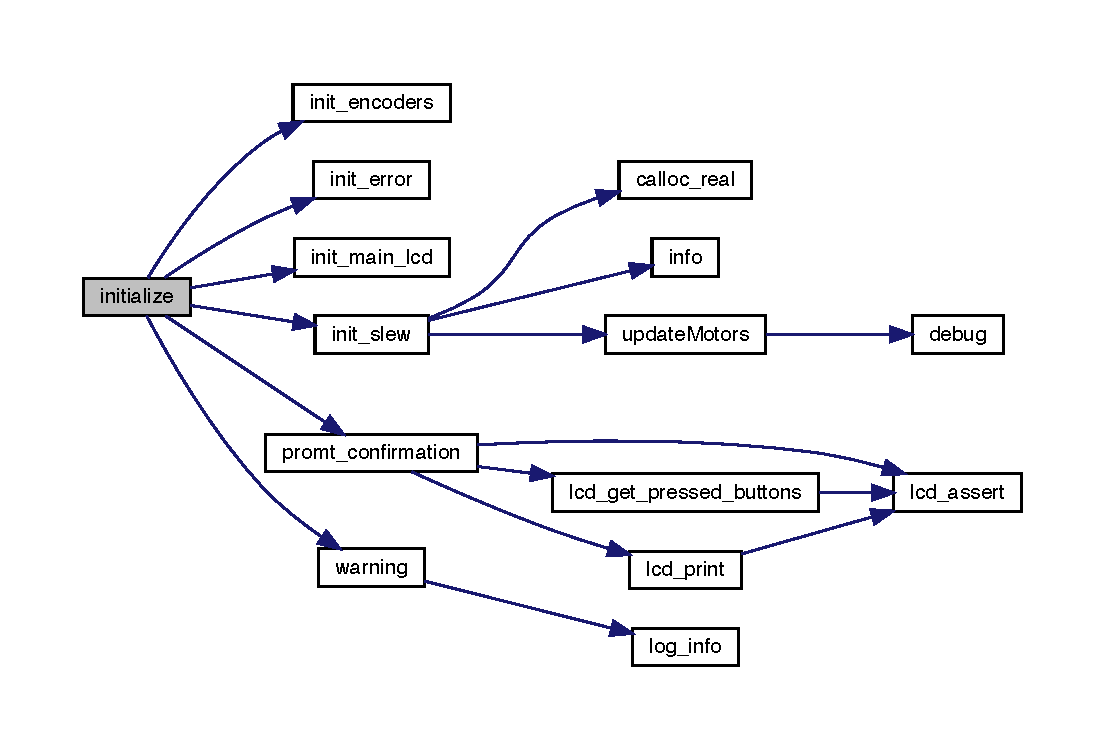
\includegraphics[width=350pt]{init_8c_a25a40b6614565f755233080a384c35f1_cgraph}
\end{center}
\end{figure}
\mbox{\label{init_8c_ad9cda921edb01125bb13c2f86bcf624b}} 
\index{init.\+c@{init.\+c}!initialize\+IO@{initialize\+IO}}
\index{initialize\+IO@{initialize\+IO}!init.\+c@{init.\+c}}
\paragraph{initialize\+I\+O()}
{\footnotesize\ttfamily void initialize\+IO (\begin{DoxyParamCaption}{ }\end{DoxyParamCaption})}



Runs pre-\/initialization code. 

This function will be started in kernel mode one time while the V\+EX Cortex is starting up. As the scheduler is still paused, most A\+PI functions will fail.

The purpose of this function is solely to set the default pin modes (\doxyref{pin\+Mode()}{p.}{_a_p_i_8h_a1875409d12eee562555bda94cad7f973}) and port states (\doxyref{digital\+Write()}{p.}{_a_p_i_8h_a23e767e5b47fa61d4e2cc02e6f15c7ab}) of limit switches, push buttons, and solenoids. It can also safely configure a U\+A\+RT port (usart\+Open()) but cannot set up an L\+CD (\doxyref{lcd\+Init()}{p.}{_a_p_i_8h_a43dc11a67b697c0d32315ea5a9af85f9}). 

Definition at line \textbf{ 36} of file \textbf{ init.\+c}.



References \textbf{ watchdog\+Init()}.


\begin{DoxyCode}
00036 \{ watchdogInit(); \}
\end{DoxyCode}
Here is the call graph for this function\+:
\nopagebreak
\begin{figure}[H]
\begin{center}
\leavevmode
\includegraphics[width=250pt]{init_8c_ad9cda921edb01125bb13c2f86bcf624b_cgraph}
\end{center}
\end{figure}


\subsubsection{Variable Documentation}
\mbox{\label{init_8c_a5dfaf05eb7e97b2e29d04eb068f9c240}} 
\index{init.\+c@{init.\+c}!lifter\+\_\+ultrasonic@{lifter\+\_\+ultrasonic}}
\index{lifter\+\_\+ultrasonic@{lifter\+\_\+ultrasonic}!init.\+c@{init.\+c}}
\paragraph{lifter\+\_\+ultrasonic}
{\footnotesize\ttfamily \textbf{ Ultrasonic} lifter\+\_\+ultrasonic}



Definition at line \textbf{ 24} of file \textbf{ sensors.\+h}.



Referenced by \textbf{ autostack\+\_\+routine()}, \textbf{ initialize()}, and \textbf{ main\+\_\+lifter\+\_\+update()}.


\hypertarget{lcd_8c}{}\section{src/lcd.c File Reference}
\label{lcd_8c}\index{src/lcd.\+c@{src/lcd.\+c}}
{\ttfamily \#include \char`\"{}lcd.\+h\char`\"{}}\newline
\subsection*{Functions}
\begin{DoxyCompactItemize}
\item 
void \hyperlink{lcd_8c_a93b26f37d6b1687ad54c90feedfd29ca}{init\+\_\+main\+\_\+lcd} (F\+I\+LE $\ast$lcd)
\begin{DoxyCompactList}\small\item\em Initializes the lcd screen. Also will initialize the lcd\+\_\+port var. Must be called before any lcd function can be called. \end{DoxyCompactList}\item 
static void \hyperlink{lcd_8c_a07f04b524b5ded617d5f193db05ba0ad}{lcd\+\_\+assert} ()
\begin{DoxyCompactList}\small\item\em Asserts the lcd is initialized Works by checking is the File $\ast$lcd\+\_\+port is the default N\+U\+LL value and thus not set. \end{DoxyCompactList}\item 
void \hyperlink{lcd_8c_a35c08b1fa742e650f4873939707b893b}{lcd\+\_\+clear} ()
\begin{DoxyCompactList}\small\item\em Clears the lcd. \end{DoxyCompactList}\item 
\hyperlink{structlcd__buttons}{lcd\+\_\+buttons} \hyperlink{lcd_8c_ac7b3225ccc82fcbe067ba9da934f010d}{lcd\+\_\+get\+\_\+pressed\+\_\+buttons} ()
\begin{DoxyCompactList}\small\item\em Returns the pressed buttons. \end{DoxyCompactList}\item 
void \hyperlink{lcd_8c_adabd3f7cdda45119604b488caf22bba8}{lcd\+\_\+print} (unsigned int line, const char $\ast$str)
\begin{DoxyCompactList}\small\item\em prints a string to a line on the lcd \end{DoxyCompactList}\item 
void \hyperlink{lcd_8c_aa0d4ca88701dfecf98796e2028482b69}{lcd\+\_\+printf} (unsigned int line, const char $\ast$format\+\_\+str,...)
\begin{DoxyCompactList}\small\item\em prints a formated string to a line on the lcd. Smilar to printf \end{DoxyCompactList}\item 
void \hyperlink{lcd_8c_a245902a4d48a6d9bd1ab308bf9b7e6b5}{lcd\+\_\+set\+\_\+backlight} (bool state)
\begin{DoxyCompactList}\small\item\em sets the backlight of the lcd \end{DoxyCompactList}\item 
void \hyperlink{lcd_8c_a99f4683e1990edf624ab216bf327cba4}{promt\+\_\+confirmation} (const char $\ast$confirm\+\_\+text)
\begin{DoxyCompactList}\small\item\em Prompts the user to confirm a string. User must press middle button to confirm. Function is not thread safe and will stall a thread. \end{DoxyCompactList}\end{DoxyCompactItemize}
\subsection*{Variables}
\begin{DoxyCompactItemize}
\item 
static F\+I\+LE $\ast$ \hyperlink{lcd_8c_a8d2a398462720032706d94d44a82a1f8}{lcd\+\_\+port} = N\+U\+LL
\end{DoxyCompactItemize}


\subsection{Function Documentation}
\mbox{\Hypertarget{lcd_8c_a93b26f37d6b1687ad54c90feedfd29ca}\label{lcd_8c_a93b26f37d6b1687ad54c90feedfd29ca}} 
\index{lcd.\+c@{lcd.\+c}!init\+\_\+main\+\_\+lcd@{init\+\_\+main\+\_\+lcd}}
\index{init\+\_\+main\+\_\+lcd@{init\+\_\+main\+\_\+lcd}!lcd.\+c@{lcd.\+c}}
\subsubsection{\texorpdfstring{init\+\_\+main\+\_\+lcd()}{init\_main\_lcd()}}
{\footnotesize\ttfamily void init\+\_\+main\+\_\+lcd (\begin{DoxyParamCaption}\item[{F\+I\+LE $\ast$}]{lcd }\end{DoxyParamCaption})}



Initializes the lcd screen. Also will initialize the lcd\+\_\+port var. Must be called before any lcd function can be called. 


\begin{DoxyParams}{Parameters}
{\em lcd} & the urart port of the lcd screen \\
\hline
\end{DoxyParams}
\begin{DoxySeeAlso}{See also}
uart1 

uart2 
\end{DoxySeeAlso}
\begin{DoxyAuthor}{Author}
Chris Jerrett 
\end{DoxyAuthor}
\begin{DoxyDate}{Date}
9/9/2017 
\end{DoxyDate}


Definition at line 39 of file lcd.\+c.



References lcd\+\_\+port.



Referenced by initialize().


\begin{DoxyCode}
39                               \{
40   lcdInit(lcd);
41   \hyperlink{lcd_8c_a8d2a398462720032706d94d44a82a1f8}{lcd\_port} = lcd;
42 \}
\end{DoxyCode}
\mbox{\Hypertarget{lcd_8c_a07f04b524b5ded617d5f193db05ba0ad}\label{lcd_8c_a07f04b524b5ded617d5f193db05ba0ad}} 
\index{lcd.\+c@{lcd.\+c}!lcd\+\_\+assert@{lcd\+\_\+assert}}
\index{lcd\+\_\+assert@{lcd\+\_\+assert}!lcd.\+c@{lcd.\+c}}
\subsubsection{\texorpdfstring{lcd\+\_\+assert()}{lcd\_assert()}}
{\footnotesize\ttfamily static void lcd\+\_\+assert (\begin{DoxyParamCaption}{ }\end{DoxyParamCaption})\hspace{0.3cm}{\ttfamily [static]}}



Asserts the lcd is initialized Works by checking is the File $\ast$lcd\+\_\+port is the default N\+U\+LL value and thus not set. 

\begin{DoxyAuthor}{Author}
Chris Jerrett 
\end{DoxyAuthor}
\begin{DoxyDate}{Date}
9/9/2017 
\end{DoxyDate}


Definition at line 13 of file lcd.\+c.



References lcd\+\_\+port.



Referenced by lcd\+\_\+clear(), lcd\+\_\+get\+\_\+pressed\+\_\+buttons(), lcd\+\_\+print(), lcd\+\_\+printf(), lcd\+\_\+set\+\_\+backlight(), and promt\+\_\+confirmation().


\begin{DoxyCode}
13                           \{
14   \textcolor{keywordflow}{if}(\hyperlink{lcd_8c_a8d2a398462720032706d94d44a82a1f8}{lcd\_port} != NULL) \{
15     printf(\textcolor{stringliteral}{"LCD NULL!"});
16     exit(1);
17   \}
18 \}
\end{DoxyCode}
\mbox{\Hypertarget{lcd_8c_a35c08b1fa742e650f4873939707b893b}\label{lcd_8c_a35c08b1fa742e650f4873939707b893b}} 
\index{lcd.\+c@{lcd.\+c}!lcd\+\_\+clear@{lcd\+\_\+clear}}
\index{lcd\+\_\+clear@{lcd\+\_\+clear}!lcd.\+c@{lcd.\+c}}
\subsubsection{\texorpdfstring{lcd\+\_\+clear()}{lcd\_clear()}}
{\footnotesize\ttfamily void lcd\+\_\+clear (\begin{DoxyParamCaption}{ }\end{DoxyParamCaption})}



Clears the lcd. 

\begin{DoxyAuthor}{Author}
Chris Jerrett 
\end{DoxyAuthor}
\begin{DoxyDate}{Date}
9/9/2017 
\end{DoxyDate}


Definition at line 34 of file lcd.\+c.



References lcd\+\_\+assert(), and lcd\+\_\+port.


\begin{DoxyCode}
34                  \{
35   \hyperlink{lcd_8c_a07f04b524b5ded617d5f193db05ba0ad}{lcd\_assert}();
36   lcdClear(\hyperlink{lcd_8c_a8d2a398462720032706d94d44a82a1f8}{lcd\_port});
37 \}
\end{DoxyCode}
\mbox{\Hypertarget{lcd_8c_ac7b3225ccc82fcbe067ba9da934f010d}\label{lcd_8c_ac7b3225ccc82fcbe067ba9da934f010d}} 
\index{lcd.\+c@{lcd.\+c}!lcd\+\_\+get\+\_\+pressed\+\_\+buttons@{lcd\+\_\+get\+\_\+pressed\+\_\+buttons}}
\index{lcd\+\_\+get\+\_\+pressed\+\_\+buttons@{lcd\+\_\+get\+\_\+pressed\+\_\+buttons}!lcd.\+c@{lcd.\+c}}
\subsubsection{\texorpdfstring{lcd\+\_\+get\+\_\+pressed\+\_\+buttons()}{lcd\_get\_pressed\_buttons()}}
{\footnotesize\ttfamily \hyperlink{structlcd__buttons}{lcd\+\_\+buttons} lcd\+\_\+get\+\_\+pressed\+\_\+buttons (\begin{DoxyParamCaption}{ }\end{DoxyParamCaption})}



Returns the pressed buttons. 

\begin{DoxyReturn}{Returns}
a struct containing the states of all three buttons. 
\end{DoxyReturn}
\begin{DoxyAuthor}{Author}
Chris Jerrett 
\end{DoxyAuthor}
\begin{DoxyDate}{Date}
9/9/2017 
\end{DoxyDate}
\begin{DoxySeeAlso}{See also}
\hyperlink{structlcd__buttons}{lcd\+\_\+buttons} 
\end{DoxySeeAlso}


Definition at line 20 of file lcd.\+c.



References lcd\+\_\+assert(), lcd\+\_\+port, lcd\+\_\+buttons\+::left, lcd\+\_\+buttons\+::middle, P\+R\+E\+S\+S\+ED, R\+E\+L\+E\+A\+S\+ED, and lcd\+\_\+buttons\+::right.



Referenced by display\+\_\+menu(), and promt\+\_\+confirmation().


\begin{DoxyCode}
20                                      \{
21   \hyperlink{lcd_8c_a07f04b524b5ded617d5f193db05ba0ad}{lcd\_assert}();
22   \textcolor{keywordtype}{unsigned} \textcolor{keywordtype}{int} btn\_binary = lcdReadButtons(\hyperlink{lcd_8c_a8d2a398462720032706d94d44a82a1f8}{lcd\_port});
23   \textcolor{keywordtype}{bool} left = btn\_binary & 0x1;
24   \textcolor{keywordtype}{bool} middle = btn\_binary & 0x2;
25   \textcolor{keywordtype}{bool} right = btn\_binary & 0x4;
26   \hyperlink{structlcd__buttons}{lcd\_buttons} btns;
27   btns.\hyperlink{structlcd__buttons_ae385efb5ec794acf5f11027f46c6c039}{left} = left ? \hyperlink{lcd_8h_a0bbab92f5605e16a4162b6c5ccc2c29ba5ef9a100ac8b4b8d6dec477c377b7901}{PRESSED} : \hyperlink{lcd_8h_a0bbab92f5605e16a4162b6c5ccc2c29baa38d18fe73a7fc82c112b6917d0b5cd0}{RELEASED};
28   btns.\hyperlink{structlcd__buttons_a293342810ac56f73979b08f144d6e6b9}{middle} = middle ? \hyperlink{lcd_8h_a0bbab92f5605e16a4162b6c5ccc2c29ba5ef9a100ac8b4b8d6dec477c377b7901}{PRESSED} : \hyperlink{lcd_8h_a0bbab92f5605e16a4162b6c5ccc2c29baa38d18fe73a7fc82c112b6917d0b5cd0}{RELEASED};
29   btns.\hyperlink{structlcd__buttons_a2437d744e09ca1bb91ab4ca53ef77198}{right} = right ? \hyperlink{lcd_8h_a0bbab92f5605e16a4162b6c5ccc2c29ba5ef9a100ac8b4b8d6dec477c377b7901}{PRESSED} : \hyperlink{lcd_8h_a0bbab92f5605e16a4162b6c5ccc2c29baa38d18fe73a7fc82c112b6917d0b5cd0}{RELEASED};
30 
31   \textcolor{keywordflow}{return} btns;
32 \}
\end{DoxyCode}
\mbox{\Hypertarget{lcd_8c_adabd3f7cdda45119604b488caf22bba8}\label{lcd_8c_adabd3f7cdda45119604b488caf22bba8}} 
\index{lcd.\+c@{lcd.\+c}!lcd\+\_\+print@{lcd\+\_\+print}}
\index{lcd\+\_\+print@{lcd\+\_\+print}!lcd.\+c@{lcd.\+c}}
\subsubsection{\texorpdfstring{lcd\+\_\+print()}{lcd\_print()}}
{\footnotesize\ttfamily void lcd\+\_\+print (\begin{DoxyParamCaption}\item[{unsigned int}]{line,  }\item[{const char $\ast$}]{str }\end{DoxyParamCaption})}



prints a string to a line on the lcd 


\begin{DoxyParams}{Parameters}
{\em line} & the line to print on \\
\hline
{\em str} & string to print \\
\hline
\end{DoxyParams}
\begin{DoxyAuthor}{Author}
Chris Jerrett 
\end{DoxyAuthor}
\begin{DoxyDate}{Date}
9/9/2017 
\end{DoxyDate}


Definition at line 44 of file lcd.\+c.



References lcd\+\_\+assert(), and lcd\+\_\+port.



Referenced by display\+\_\+menu(), and promt\+\_\+confirmation().


\begin{DoxyCode}
44                                                     \{
45   \hyperlink{lcd_8c_a07f04b524b5ded617d5f193db05ba0ad}{lcd\_assert}();
46   lcdSetText(\hyperlink{lcd_8c_a8d2a398462720032706d94d44a82a1f8}{lcd\_port}, line, str);
47 \}
\end{DoxyCode}
\mbox{\Hypertarget{lcd_8c_aa0d4ca88701dfecf98796e2028482b69}\label{lcd_8c_aa0d4ca88701dfecf98796e2028482b69}} 
\index{lcd.\+c@{lcd.\+c}!lcd\+\_\+printf@{lcd\+\_\+printf}}
\index{lcd\+\_\+printf@{lcd\+\_\+printf}!lcd.\+c@{lcd.\+c}}
\subsubsection{\texorpdfstring{lcd\+\_\+printf()}{lcd\_printf()}}
{\footnotesize\ttfamily void lcd\+\_\+printf (\begin{DoxyParamCaption}\item[{unsigned int}]{line,  }\item[{const char $\ast$}]{format\+\_\+str,  }\item[{}]{... }\end{DoxyParamCaption})}



prints a formated string to a line on the lcd. Smilar to printf 


\begin{DoxyParams}{Parameters}
{\em line} & the line to print on \\
\hline
{\em format\+\_\+str} & format string string to print \\
\hline
\end{DoxyParams}
\begin{DoxyAuthor}{Author}
Chris Jerrett 
\end{DoxyAuthor}
\begin{DoxyDate}{Date}
9/9/2017 
\end{DoxyDate}


Definition at line 49 of file lcd.\+c.



References lcd\+\_\+assert(), and lcd\+\_\+port.


\begin{DoxyCode}
49                                                                  \{
50   \hyperlink{lcd_8c_a07f04b524b5ded617d5f193db05ba0ad}{lcd\_assert}();
51   lcdPrint(\hyperlink{lcd_8c_a8d2a398462720032706d94d44a82a1f8}{lcd\_port}, line, format\_str);
52 \}
\end{DoxyCode}
\mbox{\Hypertarget{lcd_8c_a245902a4d48a6d9bd1ab308bf9b7e6b5}\label{lcd_8c_a245902a4d48a6d9bd1ab308bf9b7e6b5}} 
\index{lcd.\+c@{lcd.\+c}!lcd\+\_\+set\+\_\+backlight@{lcd\+\_\+set\+\_\+backlight}}
\index{lcd\+\_\+set\+\_\+backlight@{lcd\+\_\+set\+\_\+backlight}!lcd.\+c@{lcd.\+c}}
\subsubsection{\texorpdfstring{lcd\+\_\+set\+\_\+backlight()}{lcd\_set\_backlight()}}
{\footnotesize\ttfamily void lcd\+\_\+set\+\_\+backlight (\begin{DoxyParamCaption}\item[{bool}]{state }\end{DoxyParamCaption})}



sets the backlight of the lcd 


\begin{DoxyParams}{Parameters}
{\em state} & a boolean representing the state of the backlight. true = on, false = off. \\
\hline
\end{DoxyParams}
\begin{DoxyAuthor}{Author}
Chris Jerrett 
\end{DoxyAuthor}
\begin{DoxyDate}{Date}
9/9/2017 
\end{DoxyDate}


Definition at line 54 of file lcd.\+c.



References lcd\+\_\+assert(), and lcd\+\_\+port.


\begin{DoxyCode}
54                                     \{
55   \hyperlink{lcd_8c_a07f04b524b5ded617d5f193db05ba0ad}{lcd\_assert}();
56   lcdSetBacklight(\hyperlink{lcd_8c_a8d2a398462720032706d94d44a82a1f8}{lcd\_port}, state);
57 \}
\end{DoxyCode}
\mbox{\Hypertarget{lcd_8c_a99f4683e1990edf624ab216bf327cba4}\label{lcd_8c_a99f4683e1990edf624ab216bf327cba4}} 
\index{lcd.\+c@{lcd.\+c}!promt\+\_\+confirmation@{promt\+\_\+confirmation}}
\index{promt\+\_\+confirmation@{promt\+\_\+confirmation}!lcd.\+c@{lcd.\+c}}
\subsubsection{\texorpdfstring{promt\+\_\+confirmation()}{promt\_confirmation()}}
{\footnotesize\ttfamily void promt\+\_\+confirmation (\begin{DoxyParamCaption}\item[{const char $\ast$}]{confirm\+\_\+text }\end{DoxyParamCaption})}



Prompts the user to confirm a string. User must press middle button to confirm. Function is not thread safe and will stall a thread. 


\begin{DoxyParams}{Parameters}
{\em confirm\+\_\+text} & the text for the user to confirm. \\
\hline
\end{DoxyParams}
\begin{DoxyAuthor}{Author}
Chris Jerrett 
\end{DoxyAuthor}
\begin{DoxyDate}{Date}
9/9/2017 
\end{DoxyDate}


Definition at line 59 of file lcd.\+c.



References lcd\+\_\+assert(), lcd\+\_\+get\+\_\+pressed\+\_\+buttons(), lcd\+\_\+print(), and P\+R\+E\+S\+S\+ED.



Referenced by initialize().


\begin{DoxyCode}
59                                                   \{
60   \hyperlink{lcd_8c_a07f04b524b5ded617d5f193db05ba0ad}{lcd\_assert}();
61   \hyperlink{lcd_8c_adabd3f7cdda45119604b488caf22bba8}{lcd\_print}(1, confirm\_text);
62   \textcolor{keywordflow}{while}(\hyperlink{lcd_8c_ac7b3225ccc82fcbe067ba9da934f010d}{lcd\_get\_pressed\_buttons}().middle != \hyperlink{lcd_8h_a0bbab92f5605e16a4162b6c5ccc2c29ba5ef9a100ac8b4b8d6dec477c377b7901}{PRESSED})\{
63     delay(200);
64   \}
65 \}
\end{DoxyCode}


\subsection{Variable Documentation}
\mbox{\Hypertarget{lcd_8c_a8d2a398462720032706d94d44a82a1f8}\label{lcd_8c_a8d2a398462720032706d94d44a82a1f8}} 
\index{lcd.\+c@{lcd.\+c}!lcd\+\_\+port@{lcd\+\_\+port}}
\index{lcd\+\_\+port@{lcd\+\_\+port}!lcd.\+c@{lcd.\+c}}
\subsubsection{\texorpdfstring{lcd\+\_\+port}{lcd\_port}}
{\footnotesize\ttfamily F\+I\+LE$\ast$ lcd\+\_\+port = N\+U\+LL\hspace{0.3cm}{\ttfamily [static]}}

The port of the initialized lcd 

Definition at line 4 of file lcd.\+c.



Referenced by init\+\_\+main\+\_\+lcd(), lcd\+\_\+assert(), lcd\+\_\+clear(), lcd\+\_\+get\+\_\+pressed\+\_\+buttons(), lcd\+\_\+print(), lcd\+\_\+printf(), and lcd\+\_\+set\+\_\+backlight().


\hypertarget{log_8c}{}\section{src/log.c File Reference}
\label{log_8c}\index{src/log.\+c@{src/log.\+c}}
{\ttfamily \#include \char`\"{}log.\+h\char`\"{}}\newline
Include dependency graph for log.\+c\+:
\nopagebreak
\begin{figure}[H]
\begin{center}
\leavevmode
\includegraphics[width=149pt]{log_8c__incl}
\end{center}
\end{figure}
\subsection*{Functions}
\begin{DoxyCompactItemize}
\item 
void \hyperlink{log_8c_af3668f40d1ad1b4f3418869ac9a31f34}{debug} (const char $\ast$debug\+\_\+message)
\begin{DoxyCompactList}\small\item\em prints a info message \end{DoxyCompactList}\item 
void \hyperlink{log_8c_a8e5bb8a2a372f5b066ff7af7044584c1}{error} (const char $\ast$error\+\_\+message)
\begin{DoxyCompactList}\small\item\em prints a error message and displays on lcd. Only will print and display if log\+\_\+level is greater than N\+O\+NE \end{DoxyCompactList}\item 
void \hyperlink{log_8c_a1606d750e1bb8de9f9e917172bba3382}{info} (const char $\ast$info\+\_\+message)
\begin{DoxyCompactList}\small\item\em prints a info message \end{DoxyCompactList}\item 
void \hyperlink{log_8c_a163f389b4f5cf440a807d8fb48aaa006}{init\+\_\+error} (bool use\+\_\+lcd, F\+I\+LE $\ast$lcd)
\begin{DoxyCompactList}\small\item\em Initializes the error lcd system Only required if using lcd. \end{DoxyCompactList}\item 
static void \hyperlink{log_8c_afff22aff6749311a684a559cac3ac8bd}{log\+\_\+info} (const char $\ast$s, const char $\ast$mess)
\item 
void \hyperlink{log_8c_a0bec2cf5fff7f607bc510b74aba9887c}{warning} (const char $\ast$warning\+\_\+message)
\begin{DoxyCompactList}\small\item\em prints a warning message and displays on lcd. Only will print and display if log\+\_\+level is greater than N\+O\+NE \end{DoxyCompactList}\end{DoxyCompactItemize}
\subsection*{Variables}
\begin{DoxyCompactItemize}
\item 
static F\+I\+LE $\ast$ \hyperlink{log_8c_ac1b33b9fa813506300fa09c1b21ed20a}{log\+\_\+lcd} = N\+U\+LL
\item 
unsigned int \hyperlink{log_8c_a8cf62743dafa288b58bd7c6028ec28e5}{log\+\_\+level} = \hyperlink{log_8h_ad72dbcf6d0153db1b8d8a58001feed83}{D\+E\+B\+UG}
\end{DoxyCompactItemize}


\subsection{Function Documentation}
\mbox{\Hypertarget{log_8c_af3668f40d1ad1b4f3418869ac9a31f34}\label{log_8c_af3668f40d1ad1b4f3418869ac9a31f34}} 
\index{log.\+c@{log.\+c}!debug@{debug}}
\index{debug@{debug}!log.\+c@{log.\+c}}
\subsubsection{\texorpdfstring{debug()}{debug()}}
{\footnotesize\ttfamily void debug (\begin{DoxyParamCaption}\item[{const char $\ast$}]{debug\+\_\+message }\end{DoxyParamCaption})}



prints a info message 

Only will print and display if log\+\_\+level is greater than info \begin{DoxySeeAlso}{See also}
\hyperlink{log_8c_a8cf62743dafa288b58bd7c6028ec28e5}{log\+\_\+level} 
\end{DoxySeeAlso}

\begin{DoxyParams}{Parameters}
{\em debug\+\_\+message} & the message \\
\hline
\end{DoxyParams}


Definition at line 37 of file log.\+c.



References E\+R\+R\+OR, and log\+\_\+level.



Referenced by update\+Motors().


\begin{DoxyCode}
37                                       \{
38   \textcolor{keywordflow}{if}(\hyperlink{log_8c_a8cf62743dafa288b58bd7c6028ec28e5}{log\_level}>\hyperlink{log_8h_a8fe83ac76edc595f6b98cd4a4127aed5}{ERROR}) \{
39     printf(\textcolor{stringliteral}{"[INFO]: %s\(\backslash\)n"}, debug\_message);
40   \}
41 \}
\end{DoxyCode}
Here is the caller graph for this function\+:
\nopagebreak
\begin{figure}[H]
\begin{center}
\leavevmode
\includegraphics[width=350pt]{log_8c_af3668f40d1ad1b4f3418869ac9a31f34_icgraph}
\end{center}
\end{figure}
\mbox{\Hypertarget{log_8c_a8e5bb8a2a372f5b066ff7af7044584c1}\label{log_8c_a8e5bb8a2a372f5b066ff7af7044584c1}} 
\index{log.\+c@{log.\+c}!error@{error}}
\index{error@{error}!log.\+c@{log.\+c}}
\subsubsection{\texorpdfstring{error()}{error()}}
{\footnotesize\ttfamily void error (\begin{DoxyParamCaption}\item[{const char $\ast$}]{error\+\_\+message }\end{DoxyParamCaption})}



prints a error message and displays on lcd. Only will print and display if log\+\_\+level is greater than N\+O\+NE 

\begin{DoxySeeAlso}{See also}
\hyperlink{log_8c_a8cf62743dafa288b58bd7c6028ec28e5}{log\+\_\+level} 
\end{DoxySeeAlso}
\begin{DoxyAuthor}{Author}
Chris Jerrett 
\end{DoxyAuthor}
\begin{DoxyDate}{Date}
9/10/17 
\end{DoxyDate}

\begin{DoxyParams}{Parameters}
{\em error\+\_\+message} & the message \\
\hline
\end{DoxyParams}


Definition at line 21 of file log.\+c.



References log\+\_\+info(), log\+\_\+level, and N\+O\+NE.


\begin{DoxyCode}
21                                       \{
22   \textcolor{keywordflow}{if}(\hyperlink{log_8c_a8cf62743dafa288b58bd7c6028ec28e5}{log\_level}>\hyperlink{log_8h_a655c84af1b0034986ff56e12e84f983d}{NONE})
23     \hyperlink{log_8c_afff22aff6749311a684a559cac3ac8bd}{log\_info}(\textcolor{stringliteral}{"ERROR"}, error\_message);
24 \}
\end{DoxyCode}
Here is the call graph for this function\+:
\nopagebreak
\begin{figure}[H]
\begin{center}
\leavevmode
\includegraphics[width=204pt]{log_8c_a8e5bb8a2a372f5b066ff7af7044584c1_cgraph}
\end{center}
\end{figure}
\mbox{\Hypertarget{log_8c_a1606d750e1bb8de9f9e917172bba3382}\label{log_8c_a1606d750e1bb8de9f9e917172bba3382}} 
\index{log.\+c@{log.\+c}!info@{info}}
\index{info@{info}!log.\+c@{log.\+c}}
\subsubsection{\texorpdfstring{info()}{info()}}
{\footnotesize\ttfamily void info (\begin{DoxyParamCaption}\item[{const char $\ast$}]{info\+\_\+message }\end{DoxyParamCaption})}



prints a info message 

Only will print and display if log\+\_\+level is greater than E\+R\+R\+OR \begin{DoxySeeAlso}{See also}
\hyperlink{log_8c_a8cf62743dafa288b58bd7c6028ec28e5}{log\+\_\+level} 
\end{DoxySeeAlso}

\begin{DoxyParams}{Parameters}
{\em info\+\_\+message} & the message \\
\hline
\end{DoxyParams}


Definition at line 31 of file log.\+c.



References E\+R\+R\+OR, and log\+\_\+level.



Referenced by init\+\_\+slew().


\begin{DoxyCode}
31                                     \{
32   \textcolor{keywordflow}{if}(\hyperlink{log_8c_a8cf62743dafa288b58bd7c6028ec28e5}{log\_level}>\hyperlink{log_8h_a8fe83ac76edc595f6b98cd4a4127aed5}{ERROR}) \{
33     printf(\textcolor{stringliteral}{"[INFO]: %s\(\backslash\)n"}, info\_message);
34   \}
35 \}
\end{DoxyCode}
Here is the caller graph for this function\+:
\nopagebreak
\begin{figure}[H]
\begin{center}
\leavevmode
\includegraphics[width=290pt]{log_8c_a1606d750e1bb8de9f9e917172bba3382_icgraph}
\end{center}
\end{figure}
\mbox{\Hypertarget{log_8c_a163f389b4f5cf440a807d8fb48aaa006}\label{log_8c_a163f389b4f5cf440a807d8fb48aaa006}} 
\index{log.\+c@{log.\+c}!init\+\_\+error@{init\+\_\+error}}
\index{init\+\_\+error@{init\+\_\+error}!log.\+c@{log.\+c}}
\subsubsection{\texorpdfstring{init\+\_\+error()}{init\_error()}}
{\footnotesize\ttfamily void init\+\_\+error (\begin{DoxyParamCaption}\item[{bool}]{use\+\_\+lcd,  }\item[{F\+I\+LE $\ast$}]{lcd }\end{DoxyParamCaption})}



Initializes the error lcd system Only required if using lcd. 

\begin{DoxyAuthor}{Author}
Chris Jerrett 
\end{DoxyAuthor}
\begin{DoxyDate}{Date}
9/10/17 
\end{DoxyDate}

\begin{DoxyParams}{Parameters}
{\em use\+\_\+lcd} & whether to use the lcd \\
\hline
{\em lcd} & the lcd \\
\hline
\end{DoxyParams}


Definition at line 6 of file log.\+c.



References log\+\_\+lcd.



Referenced by initialize().


\begin{DoxyCode}
6                                          \{
7   \textcolor{keywordflow}{if}(use\_lcd) \{
8     lcdInit(lcd);
9     \hyperlink{log_8c_ac1b33b9fa813506300fa09c1b21ed20a}{log\_lcd} = lcd;
10   \}
11 \}
\end{DoxyCode}
Here is the caller graph for this function\+:
\nopagebreak
\begin{figure}[H]
\begin{center}
\leavevmode
\includegraphics[width=223pt]{log_8c_a163f389b4f5cf440a807d8fb48aaa006_icgraph}
\end{center}
\end{figure}
\mbox{\Hypertarget{log_8c_afff22aff6749311a684a559cac3ac8bd}\label{log_8c_afff22aff6749311a684a559cac3ac8bd}} 
\index{log.\+c@{log.\+c}!log\+\_\+info@{log\+\_\+info}}
\index{log\+\_\+info@{log\+\_\+info}!log.\+c@{log.\+c}}
\subsubsection{\texorpdfstring{log\+\_\+info()}{log\_info()}}
{\footnotesize\ttfamily static void log\+\_\+info (\begin{DoxyParamCaption}\item[{const char $\ast$}]{s,  }\item[{const char $\ast$}]{mess }\end{DoxyParamCaption})\hspace{0.3cm}{\ttfamily [static]}}



Definition at line 13 of file log.\+c.



References B\+O\+T\+T\+O\+M\+\_\+\+R\+OW, log\+\_\+lcd, and T\+O\+P\+\_\+\+R\+OW.



Referenced by error(), and warning().


\begin{DoxyCode}
13                                                       \{
14   printf(\textcolor{stringliteral}{"[%s]: %s\(\backslash\)n"}, s, mess);
15   lcdSetBacklight(\hyperlink{log_8c_ac1b33b9fa813506300fa09c1b21ed20a}{log\_lcd}, \textcolor{keyword}{true});
16   lcdClear(\hyperlink{log_8c_ac1b33b9fa813506300fa09c1b21ed20a}{log\_lcd});
17   lcdPrint(\hyperlink{log_8c_ac1b33b9fa813506300fa09c1b21ed20a}{log\_lcd}, \hyperlink{lcd_8h_a18bab754c6ad16bc35c48333091516c9}{TOP\_ROW}, s);
18   lcdPrint(\hyperlink{log_8c_ac1b33b9fa813506300fa09c1b21ed20a}{log\_lcd}, \hyperlink{lcd_8h_a7b55e87550874687b3e25a64e1cfda9d}{BOTTOM\_ROW}, mess);
19 \}
\end{DoxyCode}
Here is the caller graph for this function\+:
\nopagebreak
\begin{figure}[H]
\begin{center}
\leavevmode
\includegraphics[width=306pt]{log_8c_afff22aff6749311a684a559cac3ac8bd_icgraph}
\end{center}
\end{figure}
\mbox{\Hypertarget{log_8c_a0bec2cf5fff7f607bc510b74aba9887c}\label{log_8c_a0bec2cf5fff7f607bc510b74aba9887c}} 
\index{log.\+c@{log.\+c}!warning@{warning}}
\index{warning@{warning}!log.\+c@{log.\+c}}
\subsubsection{\texorpdfstring{warning()}{warning()}}
{\footnotesize\ttfamily void warning (\begin{DoxyParamCaption}\item[{const char $\ast$}]{warning\+\_\+message }\end{DoxyParamCaption})}



prints a warning message and displays on lcd. Only will print and display if log\+\_\+level is greater than N\+O\+NE 

\begin{DoxySeeAlso}{See also}
\hyperlink{log_8c_a8cf62743dafa288b58bd7c6028ec28e5}{log\+\_\+level} 
\end{DoxySeeAlso}
\begin{DoxyAuthor}{Author}
Chris Jerrett 
\end{DoxyAuthor}
\begin{DoxyDate}{Date}
9/10/17 
\end{DoxyDate}

\begin{DoxyParams}{Parameters}
{\em warning\+\_\+message} & the message \\
\hline
\end{DoxyParams}


Definition at line 26 of file log.\+c.



References log\+\_\+info(), log\+\_\+level, and W\+A\+R\+N\+I\+NG.



Referenced by initialize().


\begin{DoxyCode}
26                                           \{
27   \textcolor{keywordflow}{if}(\hyperlink{log_8c_a8cf62743dafa288b58bd7c6028ec28e5}{log\_level}>\hyperlink{log_8h_a5cb439d9f933fde4cf23caa370c030e7}{WARNING})
28     \hyperlink{log_8c_afff22aff6749311a684a559cac3ac8bd}{log\_info}(\textcolor{stringliteral}{"WARNING"}, warning\_message);
29 \}
\end{DoxyCode}
Here is the call graph for this function\+:
\nopagebreak
\begin{figure}[H]
\begin{center}
\leavevmode
\includegraphics[width=218pt]{log_8c_a0bec2cf5fff7f607bc510b74aba9887c_cgraph}
\end{center}
\end{figure}
Here is the caller graph for this function\+:
\nopagebreak
\begin{figure}[H]
\begin{center}
\leavevmode
\includegraphics[width=219pt]{log_8c_a0bec2cf5fff7f607bc510b74aba9887c_icgraph}
\end{center}
\end{figure}


\subsection{Variable Documentation}
\mbox{\Hypertarget{log_8c_ac1b33b9fa813506300fa09c1b21ed20a}\label{log_8c_ac1b33b9fa813506300fa09c1b21ed20a}} 
\index{log.\+c@{log.\+c}!log\+\_\+lcd@{log\+\_\+lcd}}
\index{log\+\_\+lcd@{log\+\_\+lcd}!log.\+c@{log.\+c}}
\subsubsection{\texorpdfstring{log\+\_\+lcd}{log\_lcd}}
{\footnotesize\ttfamily F\+I\+LE$\ast$ log\+\_\+lcd = N\+U\+LL\hspace{0.3cm}{\ttfamily [static]}}



Definition at line 4 of file log.\+c.



Referenced by init\+\_\+error(), and log\+\_\+info().

\mbox{\Hypertarget{log_8c_a8cf62743dafa288b58bd7c6028ec28e5}\label{log_8c_a8cf62743dafa288b58bd7c6028ec28e5}} 
\index{log.\+c@{log.\+c}!log\+\_\+level@{log\+\_\+level}}
\index{log\+\_\+level@{log\+\_\+level}!log.\+c@{log.\+c}}
\subsubsection{\texorpdfstring{log\+\_\+level}{log\_level}}
{\footnotesize\ttfamily unsigned int log\+\_\+level = \hyperlink{log_8h_ad72dbcf6d0153db1b8d8a58001feed83}{D\+E\+B\+UG}}



Definition at line 3 of file log.\+c.



Referenced by debug(), error(), info(), and warning().


\hypertarget{menu_8c}{}\section{src/menu.c File Reference}
\label{menu_8c}\index{src/menu.\+c@{src/menu.\+c}}
{\ttfamily \#include \char`\"{}menu.\+h\char`\"{}}\newline
Include dependency graph for menu.\+c\+:\nopagebreak
\begin{figure}[H]
\begin{center}
\leavevmode
\includegraphics[width=350pt]{menu_8c__incl}
\end{center}
\end{figure}
\subsection*{Functions}
\begin{DoxyCompactItemize}
\item 
static void \hyperlink{menu_8c_a0fb55c1213b23963d509b974d1254567}{calculate\+\_\+current\+\_\+display} (char $\ast$rtn, \hyperlink{structmenu__t}{menu\+\_\+t} $\ast$menu)
\item 
static \hyperlink{structmenu__t}{menu\+\_\+t} $\ast$ \hyperlink{menu_8c_aff4fd27ff7707295d91c67fa52a6b021}{create\+\_\+menu} (enum \hyperlink{menu_8h_a6bbf4baf5018b0d76aab6c2e6bf85e62}{menu\+\_\+type} type, const char $\ast$prompt)
\item 
void \hyperlink{menu_8c_a05a36619ac6c9ba4544eddb83ee2a50d}{denint\+\_\+menu} (\hyperlink{structmenu__t}{menu\+\_\+t} $\ast$menu)
\begin{DoxyCompactList}\small\item\em Destroys a menu {\itshape  Menu must be freed or will cause memory leak {\itshape  }}\end{DoxyCompactList}\item 
int \hyperlink{menu_8c_abfadedb104f89f672dd3045499975a71}{display\+\_\+menu} (\hyperlink{structmenu__t}{menu\+\_\+t} $\ast$menu)
\begin{DoxyCompactList}\small\item\em Displays a menu context, but does not display. {\itshape  Menu must be freed or will cause memory leak! {\itshape  Will exit if robot is enabled. This prevents menu from locking up system in even of a reset. }}\end{DoxyCompactList}\item 
\hyperlink{structmenu__t}{menu\+\_\+t} $\ast$ \hyperlink{menu_8c_a5abb752733423805f59ef3b92e3c2e57}{init\+\_\+menu\+\_\+float} (enum \hyperlink{menu_8h_a6bbf4baf5018b0d76aab6c2e6bf85e62}{menu\+\_\+type} type, float \hyperlink{vmath_8c_abd8bbcfabb3ddef2ccaafb9928a37b95}{min}, float \hyperlink{vmath_8c_af082905f7eac6d03e92015146bbc1925}{max}, float step, const char $\ast$prompt)
\begin{DoxyCompactList}\small\item\em Creates a menu context, but does not display. {\itshape  Menu must be freed or will cause memory leak! {\itshape  }}\end{DoxyCompactList}\item 
\hyperlink{structmenu__t}{menu\+\_\+t} $\ast$ \hyperlink{menu_8c_ac8efedba760ec35ebf841ab19543ba5a}{init\+\_\+menu\+\_\+int} (enum \hyperlink{menu_8h_a6bbf4baf5018b0d76aab6c2e6bf85e62}{menu\+\_\+type} type, int \hyperlink{vmath_8c_abd8bbcfabb3ddef2ccaafb9928a37b95}{min}, int \hyperlink{vmath_8c_af082905f7eac6d03e92015146bbc1925}{max}, int step, const char $\ast$prompt)
\begin{DoxyCompactList}\small\item\em Creates a menu context, but does not display. {\itshape  Menu must be freed or will cause memory leak {\itshape  }}\end{DoxyCompactList}\item 
\hyperlink{structmenu__t}{menu\+\_\+t} $\ast$ \hyperlink{menu_8c_a3529988b0a7c12cb3f2ebb3cf5595594}{init\+\_\+menu\+\_\+var} (enum \hyperlink{menu_8h_a6bbf4baf5018b0d76aab6c2e6bf85e62}{menu\+\_\+type} type, unsigned int nums, const char $\ast$prompt, char $\ast$options,...)
\begin{DoxyCompactList}\small\item\em Creates a menu context, but does not display. {\itshape  Menu must be freed or will cause memory leak {\itshape  }}\end{DoxyCompactList}\end{DoxyCompactItemize}


\subsection{Function Documentation}
\mbox{\Hypertarget{menu_8c_a0fb55c1213b23963d509b974d1254567}\label{menu_8c_a0fb55c1213b23963d509b974d1254567}} 
\index{menu.\+c@{menu.\+c}!calculate\+\_\+current\+\_\+display@{calculate\+\_\+current\+\_\+display}}
\index{calculate\+\_\+current\+\_\+display@{calculate\+\_\+current\+\_\+display}!menu.\+c@{menu.\+c}}
\subsubsection{\texorpdfstring{calculate\+\_\+current\+\_\+display()}{calculate\_current\_display()}}
{\footnotesize\ttfamily static void calculate\+\_\+current\+\_\+display (\begin{DoxyParamCaption}\item[{char $\ast$}]{rtn,  }\item[{\hyperlink{structmenu__t}{menu\+\_\+t} $\ast$}]{menu }\end{DoxyParamCaption})\hspace{0.3cm}{\ttfamily [static]}}



Definition at line 56 of file menu.\+c.



References menu\+\_\+t\+::current, F\+L\+O\+A\+T\+\_\+\+T\+Y\+PE, ftoa\+\_\+bad(), I\+N\+T\+\_\+\+T\+Y\+PE, itoa\+\_\+bad(), menu\+\_\+t\+::length, max(), menu\+\_\+t\+::max, menu\+\_\+t\+::max\+\_\+f, min(), menu\+\_\+t\+::min, menu\+\_\+t\+::min\+\_\+f, menu\+\_\+t\+::options, menu\+\_\+t\+::step, menu\+\_\+t\+::step\+\_\+f, S\+T\+R\+I\+N\+G\+\_\+\+T\+Y\+PE, and menu\+\_\+t\+::type.



Referenced by display\+\_\+menu().


\begin{DoxyCode}
56                                                                \{
57   \textcolor{keywordflow}{if}(menu->\hyperlink{structmenu__t_a110244ceb7d2a7cba95cfc5758d61c01}{type} == \hyperlink{menu_8h_a6bbf4baf5018b0d76aab6c2e6bf85e62a7823190eb356a6edf2f33589f250053c}{STRING\_TYPE})\{
58     \textcolor{comment}{//Ignore warning}
59     rtn = (menu->\hyperlink{structmenu__t_ad695cd88051e34817f0f582d4e43c33a}{options}[menu->\hyperlink{structmenu__t_a2acb18066898677ec5e2dc40eec811c5}{current} % (menu->\hyperlink{structmenu__t_a023063461c4a247e574abd6a55faf765}{length})]);
60   \}
61   \textcolor{keywordflow}{if}(menu->\hyperlink{structmenu__t_a110244ceb7d2a7cba95cfc5758d61c01}{type} == \hyperlink{menu_8h_a6bbf4baf5018b0d76aab6c2e6bf85e62a7fee88532b24b79bf2a88688a5d681d7}{INT\_TYPE}) \{
62     \textcolor{keywordtype}{int} step = (menu->\hyperlink{structmenu__t_adc50450bc59ea66a8d67424adc46e24e}{step});
63     \textcolor{keywordtype}{int} \hyperlink{vmath_8h_abd8bbcfabb3ddef2ccaafb9928a37b95}{min} = (menu->\hyperlink{structmenu__t_a6891bc6c94f1e995cc62a05b13328de5}{min});
64     \textcolor{keywordtype}{int} \hyperlink{vmath_8h_af082905f7eac6d03e92015146bbc1925}{max} = (menu->\hyperlink{structmenu__t_ace9cbaecd7bf311be0ef230da657f406}{max});
65     \textcolor{keywordtype}{int} value = menu->\hyperlink{structmenu__t_a2acb18066898677ec5e2dc40eec811c5}{current} * step;
66     value = value < min ? \hyperlink{vmath_8h_abd8bbcfabb3ddef2ccaafb9928a37b95}{min} : value;
67     value = value > max ? \hyperlink{vmath_8h_af082905f7eac6d03e92015146bbc1925}{max} : value;
68     \hyperlink{vlib_8h_a08fa7134f8b9a80eeba25f9feab22892}{itoa\_bad}(value, rtn, 4);
69   \}
70   \textcolor{keywordflow}{if}(menu->\hyperlink{structmenu__t_a110244ceb7d2a7cba95cfc5758d61c01}{type} == \hyperlink{menu_8h_a6bbf4baf5018b0d76aab6c2e6bf85e62ab2a272a88abadbaa481269e2506345c5}{FLOAT\_TYPE}) \{
71     \textcolor{keywordtype}{float} step = (menu->\hyperlink{structmenu__t_a84cfd9226f6554c63ca9f4b11f94d12d}{step\_f});
72     \textcolor{keywordtype}{float} \hyperlink{vmath_8h_abd8bbcfabb3ddef2ccaafb9928a37b95}{min} = (menu->\hyperlink{structmenu__t_a0a6e4f711992fb69e8a57c2af1ab7a05}{min\_f});
73     \textcolor{keywordtype}{float} \hyperlink{vmath_8h_af082905f7eac6d03e92015146bbc1925}{max} = (menu->\hyperlink{structmenu__t_a14b11d0a7610484462c8a6e93068a2c1}{max\_f});
74     \textcolor{keywordtype}{float} value = menu->\hyperlink{structmenu__t_a2acb18066898677ec5e2dc40eec811c5}{current} * step;
75     value = value < min ? \hyperlink{vmath_8h_abd8bbcfabb3ddef2ccaafb9928a37b95}{min} : value;
76     value = value > max ? \hyperlink{vmath_8h_af082905f7eac6d03e92015146bbc1925}{max} : value;
77 
78     \hyperlink{vlib_8h_a8805990ed667939e615e4a98950b8bd1}{ftoa\_bad}(value, rtn, 5);
79   \}
80 \}
\end{DoxyCode}
Here is the call graph for this function\+:\nopagebreak
\begin{figure}[H]
\begin{center}
\leavevmode
\includegraphics[width=350pt]{menu_8c_a0fb55c1213b23963d509b974d1254567_cgraph}
\end{center}
\end{figure}
Here is the caller graph for this function\+:\nopagebreak
\begin{figure}[H]
\begin{center}
\leavevmode
\includegraphics[width=323pt]{menu_8c_a0fb55c1213b23963d509b974d1254567_icgraph}
\end{center}
\end{figure}
\mbox{\Hypertarget{menu_8c_aff4fd27ff7707295d91c67fa52a6b021}\label{menu_8c_aff4fd27ff7707295d91c67fa52a6b021}} 
\index{menu.\+c@{menu.\+c}!create\+\_\+menu@{create\+\_\+menu}}
\index{create\+\_\+menu@{create\+\_\+menu}!menu.\+c@{menu.\+c}}
\subsubsection{\texorpdfstring{create\+\_\+menu()}{create\_menu()}}
{\footnotesize\ttfamily static \hyperlink{structmenu__t}{menu\+\_\+t} $\ast$ create\+\_\+menu (\begin{DoxyParamCaption}\item[{enum \hyperlink{menu_8h_a6bbf4baf5018b0d76aab6c2e6bf85e62}{menu\+\_\+type}}]{type,  }\item[{const char $\ast$}]{prompt }\end{DoxyParamCaption})\hspace{0.3cm}{\ttfamily [static]}}



Definition at line 6 of file menu.\+c.



References error(), menu\+\_\+t\+::max, menu\+\_\+t\+::max\+\_\+f, menu\+\_\+t\+::min, menu\+\_\+t\+::min\+\_\+f, menu\+\_\+t\+::prompt, menu\+\_\+t\+::step, menu\+\_\+t\+::step\+\_\+f, and menu\+\_\+t\+::type.



Referenced by init\+\_\+menu\+\_\+float(), init\+\_\+menu\+\_\+int(), and init\+\_\+menu\+\_\+var().


\begin{DoxyCode}
6                                                                     \{
7   \hyperlink{structmenu__t}{menu\_t}* menu = (\hyperlink{structmenu__t}{menu\_t}*) malloc(\textcolor{keyword}{sizeof}(\hyperlink{structmenu__t}{menu\_t}));
8   \textcolor{keywordflow}{if} (!menu) \{
9     \hyperlink{log_8h_a8e5bb8a2a372f5b066ff7af7044584c1}{error}(\textcolor{stringliteral}{"Menu Malloc"});
10   \}
11   menu->\hyperlink{structmenu__t_a110244ceb7d2a7cba95cfc5758d61c01}{type} = type;
12   \textcolor{comment}{// Add one for null terminator}
13   \textcolor{keywordtype}{size\_t} strlength = strlen(prompt) + 1;
14   menu->\hyperlink{structmenu__t_a7bf29a030b7ed4a623c6b445587cc647}{prompt} = (\textcolor{keywordtype}{char}*) malloc(strlength * \textcolor{keyword}{sizeof}(\textcolor{keywordtype}{char}));
15   memcpy(menu->\hyperlink{structmenu__t_a7bf29a030b7ed4a623c6b445587cc647}{prompt}, prompt, strlength);
16   menu->\hyperlink{structmenu__t_ace9cbaecd7bf311be0ef230da657f406}{max} = INT\_MAX;
17   menu->\hyperlink{structmenu__t_a6891bc6c94f1e995cc62a05b13328de5}{min} = INT\_MIN;
18   menu->\hyperlink{structmenu__t_adc50450bc59ea66a8d67424adc46e24e}{step} = 1;
19   menu->\hyperlink{structmenu__t_a0a6e4f711992fb69e8a57c2af1ab7a05}{min\_f} = FLT\_MIN;
20   menu->\hyperlink{structmenu__t_a14b11d0a7610484462c8a6e93068a2c1}{max\_f} = FLT\_MAX;
21   menu->\hyperlink{structmenu__t_a84cfd9226f6554c63ca9f4b11f94d12d}{step\_f} = 1;
22 
23   \textcolor{keywordflow}{return} menu;
24 \}
\end{DoxyCode}
Here is the call graph for this function\+:\nopagebreak
\begin{figure}[H]
\begin{center}
\leavevmode
\includegraphics[width=350pt]{menu_8c_aff4fd27ff7707295d91c67fa52a6b021_cgraph}
\end{center}
\end{figure}
Here is the caller graph for this function\+:\nopagebreak
\begin{figure}[H]
\begin{center}
\leavevmode
\includegraphics[width=274pt]{menu_8c_aff4fd27ff7707295d91c67fa52a6b021_icgraph}
\end{center}
\end{figure}
\mbox{\Hypertarget{menu_8c_a05a36619ac6c9ba4544eddb83ee2a50d}\label{menu_8c_a05a36619ac6c9ba4544eddb83ee2a50d}} 
\index{menu.\+c@{menu.\+c}!denint\+\_\+menu@{denint\+\_\+menu}}
\index{denint\+\_\+menu@{denint\+\_\+menu}!menu.\+c@{menu.\+c}}
\subsubsection{\texorpdfstring{denint\+\_\+menu()}{denint\_menu()}}
{\footnotesize\ttfamily void denint\+\_\+menu (\begin{DoxyParamCaption}\item[{\hyperlink{structmenu__t}{menu\+\_\+t} $\ast$}]{menu }\end{DoxyParamCaption})}



Destroys a menu {\itshape  Menu must be freed or will cause memory leak {\itshape  }}


\begin{DoxyParams}{Parameters}
{\em menu} & the menu to free \\
\hline
\end{DoxyParams}
\begin{DoxySeeAlso}{See also}
menu 
\end{DoxySeeAlso}
\begin{DoxyAuthor}{Author}
Chris Jerrett 
\end{DoxyAuthor}
\begin{DoxyDate}{Date}
9/8/17 
\end{DoxyDate}


Definition at line 101 of file menu.\+c.



References menu\+\_\+t\+::options, and menu\+\_\+t\+::prompt.


\begin{DoxyCode}
101                               \{
102   free(menu->\hyperlink{structmenu__t_a7bf29a030b7ed4a623c6b445587cc647}{prompt});
103   \textcolor{keywordflow}{if}(menu->\hyperlink{structmenu__t_ad695cd88051e34817f0f582d4e43c33a}{options} != NULL) free(menu->\hyperlink{structmenu__t_ad695cd88051e34817f0f582d4e43c33a}{options});
104   free(menu);
105 \}
\end{DoxyCode}
\mbox{\Hypertarget{menu_8c_abfadedb104f89f672dd3045499975a71}\label{menu_8c_abfadedb104f89f672dd3045499975a71}} 
\index{menu.\+c@{menu.\+c}!display\+\_\+menu@{display\+\_\+menu}}
\index{display\+\_\+menu@{display\+\_\+menu}!menu.\+c@{menu.\+c}}
\subsubsection{\texorpdfstring{display\+\_\+menu()}{display\_menu()}}
{\footnotesize\ttfamily int display\+\_\+menu (\begin{DoxyParamCaption}\item[{\hyperlink{structmenu__t}{menu\+\_\+t} $\ast$}]{menu }\end{DoxyParamCaption})}



Displays a menu context, but does not display. {\itshape  Menu must be freed or will cause memory leak! {\itshape  Will exit if robot is enabled. This prevents menu from locking up system in even of a reset. }}


\begin{DoxyParams}{Parameters}
{\em menu} & the menu to display \\
\hline
\end{DoxyParams}
\begin{DoxySeeAlso}{See also}
\hyperlink{menu_8h_a6bbf4baf5018b0d76aab6c2e6bf85e62}{menu\+\_\+type} 
\end{DoxySeeAlso}
\begin{DoxyAuthor}{Author}
Chris Jerrett 
\end{DoxyAuthor}
\begin{DoxyDate}{Date}
9/8/17 
\end{DoxyDate}


Definition at line 83 of file menu.\+c.



References calculate\+\_\+current\+\_\+display(), menu\+\_\+t\+::current, delay(), is\+Enabled(), lcd\+\_\+get\+\_\+pressed\+\_\+buttons(), lcd\+\_\+print(), P\+R\+E\+S\+S\+ED, menu\+\_\+t\+::prompt, R\+E\+L\+E\+A\+S\+ED, and T\+O\+P\+\_\+\+R\+OW.


\begin{DoxyCode}
83                               \{
84   \hyperlink{lcd_8h_adabd3f7cdda45119604b488caf22bba8}{lcd\_print}(\hyperlink{lcd_8h_a18bab754c6ad16bc35c48333091516c9}{TOP\_ROW}, menu->\hyperlink{structmenu__t_a7bf29a030b7ed4a623c6b445587cc647}{prompt});
85   \textcolor{comment}{//Will exit if teleop or autonomous begin. This is extremely important if robot disconnects or resets.}
86   \textcolor{keywordflow}{while}(\hyperlink{lcd_8h_ac7b3225ccc82fcbe067ba9da934f010d}{lcd\_get\_pressed\_buttons}().middle == \hyperlink{lcd_8h_a0bbab92f5605e16a4162b6c5ccc2c29baa38d18fe73a7fc82c112b6917d0b5cd0}{RELEASED} && !
      \hyperlink{_a_p_i_8h_a56722b6f1c22da04885bc9853148bb71}{isEnabled}()) \{
87     \textcolor{keywordtype}{char} val[16];
88     \hyperlink{menu_8c_a0fb55c1213b23963d509b974d1254567}{calculate\_current\_display}(val, menu);
89 
90     \textcolor{keywordflow}{if}(\hyperlink{lcd_8h_ac7b3225ccc82fcbe067ba9da934f010d}{lcd\_get\_pressed\_buttons}().right == \hyperlink{lcd_8h_a0bbab92f5605e16a4162b6c5ccc2c29ba5ef9a100ac8b4b8d6dec477c377b7901}{PRESSED}) \{
91       menu->\hyperlink{structmenu__t_a2acb18066898677ec5e2dc40eec811c5}{current} += 1;
92     \}
93     \textcolor{keywordflow}{if}(\hyperlink{lcd_8h_ac7b3225ccc82fcbe067ba9da934f010d}{lcd\_get\_pressed\_buttons}().left == \hyperlink{lcd_8h_a0bbab92f5605e16a4162b6c5ccc2c29ba5ef9a100ac8b4b8d6dec477c377b7901}{PRESSED}) \{
94       menu->\hyperlink{structmenu__t_a2acb18066898677ec5e2dc40eec811c5}{current} -= 1;
95     \}
96     \hyperlink{_a_p_i_8h_a1c59207742a1acf45a8957d7f04f9dfe}{delay}(500);
97   \}
98   \textcolor{keywordflow}{return} menu->\hyperlink{structmenu__t_a2acb18066898677ec5e2dc40eec811c5}{current};
99 \}
\end{DoxyCode}
Here is the call graph for this function\+:\nopagebreak
\begin{figure}[H]
\begin{center}
\leavevmode
\includegraphics[width=350pt]{menu_8c_abfadedb104f89f672dd3045499975a71_cgraph}
\end{center}
\end{figure}
\mbox{\Hypertarget{menu_8c_a5abb752733423805f59ef3b92e3c2e57}\label{menu_8c_a5abb752733423805f59ef3b92e3c2e57}} 
\index{menu.\+c@{menu.\+c}!init\+\_\+menu\+\_\+float@{init\+\_\+menu\+\_\+float}}
\index{init\+\_\+menu\+\_\+float@{init\+\_\+menu\+\_\+float}!menu.\+c@{menu.\+c}}
\subsubsection{\texorpdfstring{init\+\_\+menu\+\_\+float()}{init\_menu\_float()}}
{\footnotesize\ttfamily \hyperlink{structmenu__t}{menu\+\_\+t}$\ast$ init\+\_\+menu\+\_\+float (\begin{DoxyParamCaption}\item[{enum \hyperlink{menu_8h_a6bbf4baf5018b0d76aab6c2e6bf85e62}{menu\+\_\+type}}]{type,  }\item[{float}]{min,  }\item[{float}]{max,  }\item[{float}]{step,  }\item[{const char $\ast$}]{prompt }\end{DoxyParamCaption})}



Creates a menu context, but does not display. {\itshape  Menu must be freed or will cause memory leak! {\itshape  }}


\begin{DoxyParams}{Parameters}
{\em type} & the type of menu \\
\hline
\end{DoxyParams}
\begin{DoxySeeAlso}{See also}
\hyperlink{menu_8h_a6bbf4baf5018b0d76aab6c2e6bf85e62}{menu\+\_\+type} 
\end{DoxySeeAlso}

\begin{DoxyParams}{Parameters}
{\em min} & the minimum value \\
\hline
{\em max} & the maximum value \\
\hline
{\em step} & the step value \\
\hline
{\em prompt} & the prompt to display to user \\
\hline
\end{DoxyParams}
\begin{DoxyAuthor}{Author}
Chris Jerrett 
\end{DoxyAuthor}
\begin{DoxyDate}{Date}
9/8/17 
\end{DoxyDate}


Definition at line 48 of file menu.\+c.



References create\+\_\+menu(), max(), menu\+\_\+t\+::max\+\_\+f, min(), menu\+\_\+t\+::min\+\_\+f, and menu\+\_\+t\+::step\+\_\+f.


\begin{DoxyCode}
48                                                                                                   \{
49   \hyperlink{structmenu__t}{menu\_t}* menu = \hyperlink{menu_8c_aff4fd27ff7707295d91c67fa52a6b021}{create\_menu}(type, prompt);
50   menu->\hyperlink{structmenu__t_a0a6e4f711992fb69e8a57c2af1ab7a05}{min\_f} = \hyperlink{vmath_8h_abd8bbcfabb3ddef2ccaafb9928a37b95}{min};
51   menu->\hyperlink{structmenu__t_a14b11d0a7610484462c8a6e93068a2c1}{max\_f} = \hyperlink{vmath_8h_af082905f7eac6d03e92015146bbc1925}{max};
52   menu->\hyperlink{structmenu__t_a84cfd9226f6554c63ca9f4b11f94d12d}{step\_f} = step;
53   \textcolor{keywordflow}{return} menu;
54 \}
\end{DoxyCode}
Here is the call graph for this function\+:\nopagebreak
\begin{figure}[H]
\begin{center}
\leavevmode
\includegraphics[width=350pt]{menu_8c_a5abb752733423805f59ef3b92e3c2e57_cgraph}
\end{center}
\end{figure}
\mbox{\Hypertarget{menu_8c_ac8efedba760ec35ebf841ab19543ba5a}\label{menu_8c_ac8efedba760ec35ebf841ab19543ba5a}} 
\index{menu.\+c@{menu.\+c}!init\+\_\+menu\+\_\+int@{init\+\_\+menu\+\_\+int}}
\index{init\+\_\+menu\+\_\+int@{init\+\_\+menu\+\_\+int}!menu.\+c@{menu.\+c}}
\subsubsection{\texorpdfstring{init\+\_\+menu\+\_\+int()}{init\_menu\_int()}}
{\footnotesize\ttfamily \hyperlink{structmenu__t}{menu\+\_\+t}$\ast$ init\+\_\+menu\+\_\+int (\begin{DoxyParamCaption}\item[{enum \hyperlink{menu_8h_a6bbf4baf5018b0d76aab6c2e6bf85e62}{menu\+\_\+type}}]{type,  }\item[{int}]{min,  }\item[{int}]{max,  }\item[{int}]{step,  }\item[{const char $\ast$}]{prompt }\end{DoxyParamCaption})}



Creates a menu context, but does not display. {\itshape  Menu must be freed or will cause memory leak {\itshape  }}


\begin{DoxyParams}{Parameters}
{\em type} & the type of menu \\
\hline
\end{DoxyParams}
\begin{DoxySeeAlso}{See also}
\hyperlink{menu_8h_a6bbf4baf5018b0d76aab6c2e6bf85e62}{menu\+\_\+type} 
\end{DoxySeeAlso}

\begin{DoxyParams}{Parameters}
{\em min} & the minimum value \\
\hline
{\em max} & the maximum value \\
\hline
{\em step} & the step value \\
\hline
{\em prompt} & the prompt to display to user \\
\hline
\end{DoxyParams}
\begin{DoxyAuthor}{Author}
Chris Jerrett 
\end{DoxyAuthor}
\begin{DoxyDate}{Date}
9/8/17 
\end{DoxyDate}


Definition at line 40 of file menu.\+c.



References create\+\_\+menu(), max(), menu\+\_\+t\+::max, min(), menu\+\_\+t\+::min, and menu\+\_\+t\+::step.


\begin{DoxyCode}
40                                                                                           \{
41   \hyperlink{structmenu__t}{menu\_t}* menu = \hyperlink{menu_8c_aff4fd27ff7707295d91c67fa52a6b021}{create\_menu}(type, prompt);
42   menu->\hyperlink{structmenu__t_a6891bc6c94f1e995cc62a05b13328de5}{min} = \hyperlink{vmath_8h_abd8bbcfabb3ddef2ccaafb9928a37b95}{min};
43   menu->\hyperlink{structmenu__t_ace9cbaecd7bf311be0ef230da657f406}{max} = \hyperlink{vmath_8h_af082905f7eac6d03e92015146bbc1925}{max};
44   menu->\hyperlink{structmenu__t_adc50450bc59ea66a8d67424adc46e24e}{step} = step;
45   \textcolor{keywordflow}{return} menu;
46 \}
\end{DoxyCode}
Here is the call graph for this function\+:\nopagebreak
\begin{figure}[H]
\begin{center}
\leavevmode
\includegraphics[width=350pt]{menu_8c_ac8efedba760ec35ebf841ab19543ba5a_cgraph}
\end{center}
\end{figure}
\mbox{\Hypertarget{menu_8c_a3529988b0a7c12cb3f2ebb3cf5595594}\label{menu_8c_a3529988b0a7c12cb3f2ebb3cf5595594}} 
\index{menu.\+c@{menu.\+c}!init\+\_\+menu\+\_\+var@{init\+\_\+menu\+\_\+var}}
\index{init\+\_\+menu\+\_\+var@{init\+\_\+menu\+\_\+var}!menu.\+c@{menu.\+c}}
\subsubsection{\texorpdfstring{init\+\_\+menu\+\_\+var()}{init\_menu\_var()}}
{\footnotesize\ttfamily \hyperlink{structmenu__t}{menu\+\_\+t}$\ast$ init\+\_\+menu\+\_\+var (\begin{DoxyParamCaption}\item[{enum \hyperlink{menu_8h_a6bbf4baf5018b0d76aab6c2e6bf85e62}{menu\+\_\+type}}]{type,  }\item[{unsigned int}]{nums,  }\item[{const char $\ast$}]{prompt,  }\item[{char $\ast$}]{options,  }\item[{}]{... }\end{DoxyParamCaption})}



Creates a menu context, but does not display. {\itshape  Menu must be freed or will cause memory leak {\itshape  }}


\begin{DoxyParams}{Parameters}
{\em type} & the type of menu \\
\hline
\end{DoxyParams}
\begin{DoxySeeAlso}{See also}
\hyperlink{menu_8h_a6bbf4baf5018b0d76aab6c2e6bf85e62}{menu\+\_\+type} 
\end{DoxySeeAlso}

\begin{DoxyParams}{Parameters}
{\em nums} & the number of elements passed to function \\
\hline
{\em prompt} & the prompt to display to user \\
\hline
{\em options} & the options to display for user \\
\hline
\end{DoxyParams}
\begin{DoxyAuthor}{Author}
Chris Jerrett 
\end{DoxyAuthor}
\begin{DoxyDate}{Date}
9/8/17 
\end{DoxyDate}


Definition at line 26 of file menu.\+c.



References calloc\+\_\+real(), create\+\_\+menu(), menu\+\_\+t\+::length, and menu\+\_\+t\+::options.


\begin{DoxyCode}
26                                                                                                     \{
27   \hyperlink{structmenu__t}{menu\_t}* menu = \hyperlink{menu_8c_aff4fd27ff7707295d91c67fa52a6b021}{create\_menu}(type, prompt);
28   va\_list values;
29   \textcolor{keywordtype}{char} **options\_array = (\textcolor{keywordtype}{char}**)\hyperlink{vlib_8h_a1115803c6996aebfbf67434810df7b4b}{calloc\_real}(\textcolor{keyword}{sizeof}(\textcolor{keywordtype}{char}*), nums);
30   va\_start(values, options);
31   \textcolor{keywordflow}{for}(\textcolor{keywordtype}{unsigned} \textcolor{keywordtype}{int} i = 0; i < nums; i++)\{
32     options\_array[i] = va\_arg(values, \textcolor{keywordtype}{char}*);
33   \}
34   va\_end(values);
35   menu->\hyperlink{structmenu__t_ad695cd88051e34817f0f582d4e43c33a}{options} = options\_array;
36   menu->\hyperlink{structmenu__t_a023063461c4a247e574abd6a55faf765}{length} = nums;
37   \textcolor{keywordflow}{return} menu;
38 \}
\end{DoxyCode}
Here is the call graph for this function\+:\nopagebreak
\begin{figure}[H]
\begin{center}
\leavevmode
\includegraphics[width=350pt]{menu_8c_a3529988b0a7c12cb3f2ebb3cf5595594_cgraph}
\end{center}
\end{figure}

\hypertarget{opcontrol_8c}{}\section{src/opcontrol.c File Reference}
\label{opcontrol_8c}\index{src/opcontrol.\+c@{src/opcontrol.\+c}}


File for operator control code.  


{\ttfamily \#include \char`\"{}main.\+h\char`\"{}}\newline
{\ttfamily \#include \char`\"{}slew.\+h\char`\"{}}\newline
{\ttfamily \#include \char`\"{}drive.\+h\char`\"{}}\newline
{\ttfamily \#include \char`\"{}lifter.\+h\char`\"{}}\newline
{\ttfamily \#include \char`\"{}localization.\+h\char`\"{}}\newline
{\ttfamily \#include \char`\"{}claw.\+h\char`\"{}}\newline
{\ttfamily \#include \char`\"{}mobile\+\_\+goal\+\_\+intake.\+h\char`\"{}}\newline
{\ttfamily \#include \char`\"{}vmath.\+h\char`\"{}}\newline
Include dependency graph for opcontrol.\+c\+:
\nopagebreak
\begin{figure}[H]
\begin{center}
\leavevmode
\includegraphics[width=350pt]{opcontrol_8c__incl}
\end{center}
\end{figure}
\subsection*{Functions}
\begin{DoxyCompactItemize}
\item 
void \hyperlink{opcontrol_8c_ac71a94af413917f27d108e95c4d6f6a7}{operator\+Control} ()
\end{DoxyCompactItemize}


\subsection{Detailed Description}
File for operator control code. 

This file should contain the user \hyperlink{opcontrol_8c_ac71a94af413917f27d108e95c4d6f6a7}{operator\+Control()} function and any functions related to it.

Any copyright is dedicated to the Public Domain. \href{http://creativecommons.org/publicdomain/zero/1.0/}{\tt http\+://creativecommons.\+org/publicdomain/zero/1.\+0/}

P\+R\+OS contains Free\+R\+T\+OS (\href{http://www.freertos.org}{\tt http\+://www.\+freertos.\+org}) whose source code may be obtained from \href{http://sourceforge.net/projects/freertos/files/}{\tt http\+://sourceforge.\+net/projects/freertos/files/} or on request. 

\subsection{Function Documentation}
\mbox{\Hypertarget{opcontrol_8c_ac71a94af413917f27d108e95c4d6f6a7}\label{opcontrol_8c_ac71a94af413917f27d108e95c4d6f6a7}} 
\index{opcontrol.\+c@{opcontrol.\+c}!operator\+Control@{operator\+Control}}
\index{operator\+Control@{operator\+Control}!opcontrol.\+c@{opcontrol.\+c}}
\subsubsection{\texorpdfstring{operator\+Control()}{operatorControl()}}
{\footnotesize\ttfamily void operator\+Control (\begin{DoxyParamCaption}{ }\end{DoxyParamCaption})}

Runs the user operator control code. This function will be started in its own task with the default priority and stack size whenever the robot is enabled via the Field Management System or the V\+EX Competition Switch in the operator control mode. If the robot is disabled or communications is lost, the operator control task will be stopped by the kernel. Re-\/enabling the robot will restart the task, not resume it from where it left off.

If no V\+EX Competition Switch or Field Management system is plugged in, the V\+EX Cortex will run the operator control task. Be warned that this will also occur if the V\+EX Cortex is tethered directly to a computer via the U\+SB A to A cable without any V\+EX Joystick attached.

Code running in this task can take almost any action, as the V\+EX Joystick is available and the scheduler is operational. However, proper use of \hyperlink{_a_p_i_8h_a1c59207742a1acf45a8957d7f04f9dfe}{delay()} or \hyperlink{_a_p_i_8h_ae93bc867b1aa4a12d6536a497f1b6869}{task\+Delay\+Until()} is highly recommended to give other tasks (including system tasks such as updating L\+C\+Ds) time to run.

This task should never exit; it should end with some kind of infinite loop, even if empty. 

Definition at line 40 of file opcontrol.\+c.



References delay(), init\+\_\+slew(), update\+\_\+claw(), update\+\_\+control(), update\+\_\+drive\+\_\+motors(), update\+\_\+lifter(), and update\+Intake().


\begin{DoxyCode}
40                        \{
41     \hyperlink{slew_8h_a321758941d88b75783955c819bb75005}{init\_slew}();
42     \hyperlink{_a_p_i_8h_a1c59207742a1acf45a8957d7f04f9dfe}{delay}(10);
43     \textcolor{keywordflow}{while} (1) \{
44         \hyperlink{drive_8h_a8224a4626a934d30ed587671b7004bf8}{update\_drive\_motors}();
45         \hyperlink{lifter_8h_a59bb7413777ca16aba124aaedf95c79b}{update\_lifter}();
46         \hyperlink{claw_8h_a0122b78972344264b8a276a559cfce4a}{update\_claw}();
47         \hyperlink{mobile__goal__intake_8h_ad0232c21c5c1ffda603d2b7d61034118}{updateIntake}();
48         \hyperlink{partner_8h_ab2c78903a76d2ed8969271803c78368a}{update\_control}();
49         \hyperlink{_a_p_i_8h_a1c59207742a1acf45a8957d7f04f9dfe}{delay}(25);
50     \}
51 \}
\end{DoxyCode}
Here is the call graph for this function\+:\nopagebreak
\begin{figure}[H]
\begin{center}
\leavevmode
\includegraphics[width=350pt]{opcontrol_8c_ac71a94af413917f27d108e95c4d6f6a7_cgraph}
\end{center}
\end{figure}

\hypertarget{slew_8c}{}\section{src/slew.c File Reference}
\label{slew_8c}\index{src/slew.\+c@{src/slew.\+c}}
{\ttfamily \#include \char`\"{}slew.\+h\char`\"{}}\newline
{\ttfamily \#include \char`\"{}log.\+h\char`\"{}}\newline
Include dependency graph for slew.\+c\+:\nopagebreak
\begin{figure}[H]
\begin{center}
\leavevmode
\includegraphics[width=350pt]{slew_8c__incl}
\end{center}
\end{figure}
\subsection*{Functions}
\begin{DoxyCompactItemize}
\item 
void \hyperlink{slew_8c_a981c9990a969d2587e66e550737f7cd9}{deinitslew} ()
\begin{DoxyCompactList}\small\item\em Deinitializes the slew rate controller and frees memory. \end{DoxyCompactList}\item 
void \hyperlink{slew_8c_a321758941d88b75783955c819bb75005}{init\+\_\+slew} ()
\begin{DoxyCompactList}\small\item\em Initializes the slew rate controller. \end{DoxyCompactList}\item 
void \hyperlink{slew_8c_a9f8b8ae577ef938622024545711f0151}{set\+\_\+motor\+\_\+immediate} (int motor, int speed)
\item 
void \hyperlink{slew_8c_a7dff2b79dffe55fb936d977594d7c01d}{set\+\_\+motor\+\_\+slew} (int motor, int speed)
\begin{DoxyCompactList}\small\item\em Sets motor speed wrapped inside the slew rate controller. \end{DoxyCompactList}\item 
void \hyperlink{slew_8c_a807a87c5df438fde21c1e8213906695b}{update\+Motors} ()
\begin{DoxyCompactList}\small\item\em Closes the distance between the desired motor value and the current motor value by half for each motor. \end{DoxyCompactList}\end{DoxyCompactItemize}
\subsection*{Variables}
\begin{DoxyCompactItemize}
\item 
static bool \hyperlink{slew_8c_aedeffc7d23da25d52b9a50045189fe2b}{initialized} = false
\item 
static int \hyperlink{slew_8c_a69e0d1204ea4d87b7366c9cd79527984}{motors\+\_\+curr\+\_\+speeds} \mbox{[}10\mbox{]}
\item 
static int \hyperlink{slew_8c_acf7558ed17fdecd298ea7eb82291c7d0}{motors\+\_\+set\+\_\+speeds} \mbox{[}10\mbox{]}
\item 
static \hyperlink{_a_p_i_8h_a23dca3c0de10682afb982677ff292f77}{Task\+Handle} \hyperlink{slew_8c_a9dc30877eadbb32ceb6bede027c9a93f}{slew} = N\+U\+LL
\item 
static \hyperlink{_a_p_i_8h_a9b40607ca13d2b5261f47f613e3c4fa4}{Mutex} \hyperlink{slew_8c_a29ddd4c66a52ff81b441d04f9f6d9318}{speeds\+\_\+mutex}
\end{DoxyCompactItemize}


\subsection{Function Documentation}
\mbox{\Hypertarget{slew_8c_a981c9990a969d2587e66e550737f7cd9}\label{slew_8c_a981c9990a969d2587e66e550737f7cd9}} 
\index{slew.\+c@{slew.\+c}!deinitslew@{deinitslew}}
\index{deinitslew@{deinitslew}!slew.\+c@{slew.\+c}}
\subsubsection{\texorpdfstring{deinitslew()}{deinitslew()}}
{\footnotesize\ttfamily void deinitslew (\begin{DoxyParamCaption}{ }\end{DoxyParamCaption})}



Deinitializes the slew rate controller and frees memory. 

\begin{DoxyAuthor}{Author}
Chris Jerrett 
\end{DoxyAuthor}
\begin{DoxyDate}{Date}
9/14/17 
\end{DoxyDate}


Definition at line 43 of file slew.\+c.



References initialized, motors\+\_\+curr\+\_\+speeds, motors\+\_\+set\+\_\+speeds, slew, and task\+Delete().



Referenced by autonomous().


\begin{DoxyCode}
43                  \{
44   \hyperlink{_a_p_i_8h_add3b8d580ea6ef5635c6d9ff88c68612}{taskDelete}(\hyperlink{slew_8c_a9dc30877eadbb32ceb6bede027c9a93f}{slew});
45   memset(\hyperlink{slew_8c_acf7558ed17fdecd298ea7eb82291c7d0}{motors\_set\_speeds}, 0, \textcolor{keyword}{sizeof}(\textcolor{keywordtype}{int}) * 10);
46   memset(\hyperlink{slew_8c_a69e0d1204ea4d87b7366c9cd79527984}{motors\_curr\_speeds}, 0, \textcolor{keyword}{sizeof}(\textcolor{keywordtype}{int}) * 10);
47   \hyperlink{slew_8c_aedeffc7d23da25d52b9a50045189fe2b}{initialized} = \textcolor{keyword}{false};
48 \}
\end{DoxyCode}
Here is the call graph for this function\+:\nopagebreak
\begin{figure}[H]
\begin{center}
\leavevmode
\includegraphics[width=239pt]{slew_8c_a981c9990a969d2587e66e550737f7cd9_cgraph}
\end{center}
\end{figure}
Here is the caller graph for this function\+:\nopagebreak
\begin{figure}[H]
\begin{center}
\leavevmode
\includegraphics[width=247pt]{slew_8c_a981c9990a969d2587e66e550737f7cd9_icgraph}
\end{center}
\end{figure}
\mbox{\Hypertarget{slew_8c_a321758941d88b75783955c819bb75005}\label{slew_8c_a321758941d88b75783955c819bb75005}} 
\index{slew.\+c@{slew.\+c}!init\+\_\+slew@{init\+\_\+slew}}
\index{init\+\_\+slew@{init\+\_\+slew}!slew.\+c@{slew.\+c}}
\subsubsection{\texorpdfstring{init\+\_\+slew()}{init\_slew()}}
{\footnotesize\ttfamily void init\+\_\+slew (\begin{DoxyParamCaption}{ }\end{DoxyParamCaption})}



Initializes the slew rate controller. 

\begin{DoxyAuthor}{Author}
Chris Jerrett, Christian De\+Simone 
\end{DoxyAuthor}
\begin{DoxyDate}{Date}
9/14/17 
\end{DoxyDate}


Definition at line 30 of file slew.\+c.



References info(), initialized, motors\+\_\+curr\+\_\+speeds, motors\+\_\+set\+\_\+speeds, motor\+Stop\+All(), mutex\+Create(), slew, speeds\+\_\+mutex, task\+Run\+Loop(), update\+Motors(), and warning().



Referenced by autonomous(), operator\+Control(), set\+\_\+motor\+\_\+immediate(), and set\+\_\+motor\+\_\+slew().


\begin{DoxyCode}
30                 \{
31   \textcolor{keywordflow}{if}(\hyperlink{slew_8c_aedeffc7d23da25d52b9a50045189fe2b}{initialized}) \{
32     \hyperlink{log_8h_a0bec2cf5fff7f607bc510b74aba9887c}{warning}(\textcolor{stringliteral}{"Trying to init already init slew"});
33   \}
34   memset(\hyperlink{slew_8c_acf7558ed17fdecd298ea7eb82291c7d0}{motors\_set\_speeds}, 0, \textcolor{keyword}{sizeof}(\textcolor{keywordtype}{int}) * 10);
35   memset(\hyperlink{slew_8c_a69e0d1204ea4d87b7366c9cd79527984}{motors\_curr\_speeds}, 0, \textcolor{keyword}{sizeof}(\textcolor{keywordtype}{int}) * 10);
36   \hyperlink{_a_p_i_8h_a8966c541f3e9565aea1289f0d2f2cf43}{motorStopAll}();
37   \hyperlink{log_8h_a1606d750e1bb8de9f9e917172bba3382}{info}(\textcolor{stringliteral}{"Did Init Slew"});
38   \hyperlink{slew_8c_a29ddd4c66a52ff81b441d04f9f6d9318}{speeds\_mutex} = \hyperlink{_a_p_i_8h_aecd027ce8f8b52a765735e9eb5b202b3}{mutexCreate}();
39   \hyperlink{slew_8c_a9dc30877eadbb32ceb6bede027c9a93f}{slew} = \hyperlink{_a_p_i_8h_ab05a241d6d1fd98b1ceb4665db678156}{taskRunLoop}(\hyperlink{slew_8c_a807a87c5df438fde21c1e8213906695b}{updateMotors}, 100);
40   \hyperlink{slew_8c_aedeffc7d23da25d52b9a50045189fe2b}{initialized} = \textcolor{keyword}{true};
41 \}
\end{DoxyCode}
Here is the call graph for this function\+:\nopagebreak
\begin{figure}[H]
\begin{center}
\leavevmode
\includegraphics[width=350pt]{slew_8c_a321758941d88b75783955c819bb75005_cgraph}
\end{center}
\end{figure}
Here is the caller graph for this function\+:\nopagebreak
\begin{figure}[H]
\begin{center}
\leavevmode
\includegraphics[width=350pt]{slew_8c_a321758941d88b75783955c819bb75005_icgraph}
\end{center}
\end{figure}
\mbox{\Hypertarget{slew_8c_a9f8b8ae577ef938622024545711f0151}\label{slew_8c_a9f8b8ae577ef938622024545711f0151}} 
\index{slew.\+c@{slew.\+c}!set\+\_\+motor\+\_\+immediate@{set\+\_\+motor\+\_\+immediate}}
\index{set\+\_\+motor\+\_\+immediate@{set\+\_\+motor\+\_\+immediate}!slew.\+c@{slew.\+c}}
\subsubsection{\texorpdfstring{set\+\_\+motor\+\_\+immediate()}{set\_motor\_immediate()}}
{\footnotesize\ttfamily void set\+\_\+motor\+\_\+immediate (\begin{DoxyParamCaption}\item[{int}]{motor,  }\item[{int}]{speed }\end{DoxyParamCaption})}



Definition at line 60 of file slew.\+c.



References debug(), init\+\_\+slew(), initialized, motors\+\_\+curr\+\_\+speeds, motors\+\_\+set\+\_\+speeds, motor\+Set(), mutex\+Give(), mutex\+Take(), and speeds\+\_\+mutex.



Referenced by close\+\_\+claw(), open\+\_\+claw(), set\+\_\+claw\+\_\+motor(), set\+\_\+intake\+\_\+motor(), and set\+\_\+lifter\+\_\+motors().


\begin{DoxyCode}
60                                                \{
61   \textcolor{keywordflow}{if}(!\hyperlink{slew_8c_aedeffc7d23da25d52b9a50045189fe2b}{initialized}) \{
62     \hyperlink{log_8h_af3668f40d1ad1b4f3418869ac9a31f34}{debug}(\textcolor{stringliteral}{"Slew Not Initialized! Initializing"});
63     \hyperlink{slew_8c_a321758941d88b75783955c819bb75005}{init\_slew}();
64   \}
65   \hyperlink{_a_p_i_8h_a03c5b04b472d024281f62d7af8854a8e}{motorSet}(motor, speed);
66   \hyperlink{_a_p_i_8h_a8b51124628d2a7741738d48551d1e8ee}{mutexTake}(\hyperlink{slew_8c_a29ddd4c66a52ff81b441d04f9f6d9318}{speeds\_mutex}, 10);
67   \hyperlink{slew_8c_a69e0d1204ea4d87b7366c9cd79527984}{motors\_curr\_speeds}[motor-1] = speed;
68   \hyperlink{slew_8c_acf7558ed17fdecd298ea7eb82291c7d0}{motors\_set\_speeds}[motor-1] = speed;
69   \hyperlink{_a_p_i_8h_afe171a08d22de18fc2ab604b2364959f}{mutexGive}(\hyperlink{slew_8c_a29ddd4c66a52ff81b441d04f9f6d9318}{speeds\_mutex});
70 \}
\end{DoxyCode}
Here is the call graph for this function\+:\nopagebreak
\begin{figure}[H]
\begin{center}
\leavevmode
\includegraphics[width=350pt]{slew_8c_a9f8b8ae577ef938622024545711f0151_cgraph}
\end{center}
\end{figure}
Here is the caller graph for this function\+:\nopagebreak
\begin{figure}[H]
\begin{center}
\leavevmode
\includegraphics[width=350pt]{slew_8c_a9f8b8ae577ef938622024545711f0151_icgraph}
\end{center}
\end{figure}
\mbox{\Hypertarget{slew_8c_a7dff2b79dffe55fb936d977594d7c01d}\label{slew_8c_a7dff2b79dffe55fb936d977594d7c01d}} 
\index{slew.\+c@{slew.\+c}!set\+\_\+motor\+\_\+slew@{set\+\_\+motor\+\_\+slew}}
\index{set\+\_\+motor\+\_\+slew@{set\+\_\+motor\+\_\+slew}!slew.\+c@{slew.\+c}}
\subsubsection{\texorpdfstring{set\+\_\+motor\+\_\+slew()}{set\_motor\_slew()}}
{\footnotesize\ttfamily void set\+\_\+motor\+\_\+slew (\begin{DoxyParamCaption}\item[{int}]{motor,  }\item[{int}]{speed }\end{DoxyParamCaption})}



Sets motor speed wrapped inside the slew rate controller. 


\begin{DoxyParams}{Parameters}
{\em motor} & the motor port to use \\
\hline
{\em speed} & the speed to use, between -\/127 and 127 \\
\hline
\end{DoxyParams}
\begin{DoxyAuthor}{Author}
Chris Jerrett 
\end{DoxyAuthor}
\begin{DoxyDate}{Date}
9/14/17 
\end{DoxyDate}


Definition at line 50 of file slew.\+c.



References debug(), init\+\_\+slew(), initialized, motors\+\_\+set\+\_\+speeds, mutex\+Give(), mutex\+Take(), and speeds\+\_\+mutex.



Referenced by set\+\_\+side\+\_\+speed().


\begin{DoxyCode}
50                                          \{
51   \textcolor{keywordflow}{if}(!\hyperlink{slew_8c_aedeffc7d23da25d52b9a50045189fe2b}{initialized}) \{
52     \hyperlink{log_8h_af3668f40d1ad1b4f3418869ac9a31f34}{debug}(\textcolor{stringliteral}{"Slew Not Initialized! Initializing"});
53     \hyperlink{slew_8c_a321758941d88b75783955c819bb75005}{init\_slew}();
54   \}
55   \hyperlink{_a_p_i_8h_a8b51124628d2a7741738d48551d1e8ee}{mutexTake}(\hyperlink{slew_8c_a29ddd4c66a52ff81b441d04f9f6d9318}{speeds\_mutex}, 10);
56   \hyperlink{slew_8c_acf7558ed17fdecd298ea7eb82291c7d0}{motors\_set\_speeds}[motor-1] = speed;
57   \hyperlink{_a_p_i_8h_afe171a08d22de18fc2ab604b2364959f}{mutexGive}(\hyperlink{slew_8c_a29ddd4c66a52ff81b441d04f9f6d9318}{speeds\_mutex});
58 \}
\end{DoxyCode}
Here is the call graph for this function\+:\nopagebreak
\begin{figure}[H]
\begin{center}
\leavevmode
\includegraphics[width=350pt]{slew_8c_a7dff2b79dffe55fb936d977594d7c01d_cgraph}
\end{center}
\end{figure}
Here is the caller graph for this function\+:\nopagebreak
\begin{figure}[H]
\begin{center}
\leavevmode
\includegraphics[width=350pt]{slew_8c_a7dff2b79dffe55fb936d977594d7c01d_icgraph}
\end{center}
\end{figure}
\mbox{\Hypertarget{slew_8c_a807a87c5df438fde21c1e8213906695b}\label{slew_8c_a807a87c5df438fde21c1e8213906695b}} 
\index{slew.\+c@{slew.\+c}!update\+Motors@{update\+Motors}}
\index{update\+Motors@{update\+Motors}!slew.\+c@{slew.\+c}}
\subsubsection{\texorpdfstring{update\+Motors()}{updateMotors()}}
{\footnotesize\ttfamily void update\+Motors (\begin{DoxyParamCaption}{ }\end{DoxyParamCaption})}



Closes the distance between the desired motor value and the current motor value by half for each motor. 

\begin{DoxyAuthor}{Author}
Chris Jerrett 
\end{DoxyAuthor}
\begin{DoxyDate}{Date}
9/14/17 
\end{DoxyDate}


Definition at line 13 of file slew.\+c.



References motors\+\_\+curr\+\_\+speeds, motors\+\_\+set\+\_\+speeds, motor\+Set(), mutex\+Give(), mutex\+Take(), and speeds\+\_\+mutex.



Referenced by init\+\_\+slew().


\begin{DoxyCode}
13                    \{
14   \textcolor{comment}{//Take back half approach}
15   \textcolor{comment}{//Not linear but equal to setSpeed(1-(1/2)^x)}
16   \textcolor{keywordflow}{for}(\textcolor{keywordtype}{unsigned} \textcolor{keywordtype}{int} i = 0; i < 9; i++) \{
17     \textcolor{keywordflow}{if}(\hyperlink{slew_8c_acf7558ed17fdecd298ea7eb82291c7d0}{motors\_set\_speeds}[i] == \hyperlink{slew_8c_a69e0d1204ea4d87b7366c9cd79527984}{motors\_curr\_speeds}[i]) \textcolor{keywordflow}{continue};
18     \hyperlink{_a_p_i_8h_a8b51124628d2a7741738d48551d1e8ee}{mutexTake}(\hyperlink{slew_8c_a29ddd4c66a52ff81b441d04f9f6d9318}{speeds\_mutex}, 10);
19     \textcolor{keywordtype}{int} set\_speed = (\hyperlink{slew_8c_acf7558ed17fdecd298ea7eb82291c7d0}{motors\_set\_speeds}[i]);
20     \textcolor{keywordtype}{int} curr\_speed = \hyperlink{slew_8c_a69e0d1204ea4d87b7366c9cd79527984}{motors\_curr\_speeds}[i];
21     \hyperlink{_a_p_i_8h_afe171a08d22de18fc2ab604b2364959f}{mutexGive}(\hyperlink{slew_8c_a29ddd4c66a52ff81b441d04f9f6d9318}{speeds\_mutex});
22     \textcolor{keywordtype}{int} diff = set\_speed - curr\_speed;
23     \textcolor{keywordtype}{int} offset = diff;
24     \textcolor{keywordtype}{int} n = curr\_speed + offset;
25     \hyperlink{slew_8c_a69e0d1204ea4d87b7366c9cd79527984}{motors\_curr\_speeds}[i] = n;
26     \hyperlink{_a_p_i_8h_a03c5b04b472d024281f62d7af8854a8e}{motorSet}(i+1, n);
27   \}
28 \}
\end{DoxyCode}
Here is the call graph for this function\+:\nopagebreak
\begin{figure}[H]
\begin{center}
\leavevmode
\includegraphics[width=258pt]{slew_8c_a807a87c5df438fde21c1e8213906695b_cgraph}
\end{center}
\end{figure}
Here is the caller graph for this function\+:\nopagebreak
\begin{figure}[H]
\begin{center}
\leavevmode
\includegraphics[width=350pt]{slew_8c_a807a87c5df438fde21c1e8213906695b_icgraph}
\end{center}
\end{figure}


\subsection{Variable Documentation}
\mbox{\Hypertarget{slew_8c_aedeffc7d23da25d52b9a50045189fe2b}\label{slew_8c_aedeffc7d23da25d52b9a50045189fe2b}} 
\index{slew.\+c@{slew.\+c}!initialized@{initialized}}
\index{initialized@{initialized}!slew.\+c@{slew.\+c}}
\subsubsection{\texorpdfstring{initialized}{initialized}}
{\footnotesize\ttfamily bool initialized = false\hspace{0.3cm}{\ttfamily [static]}}



Definition at line 11 of file slew.\+c.



Referenced by deinitslew(), init\+\_\+slew(), set\+\_\+motor\+\_\+immediate(), and set\+\_\+motor\+\_\+slew().

\mbox{\Hypertarget{slew_8c_a69e0d1204ea4d87b7366c9cd79527984}\label{slew_8c_a69e0d1204ea4d87b7366c9cd79527984}} 
\index{slew.\+c@{slew.\+c}!motors\+\_\+curr\+\_\+speeds@{motors\+\_\+curr\+\_\+speeds}}
\index{motors\+\_\+curr\+\_\+speeds@{motors\+\_\+curr\+\_\+speeds}!slew.\+c@{slew.\+c}}
\subsubsection{\texorpdfstring{motors\+\_\+curr\+\_\+speeds}{motors\_curr\_speeds}}
{\footnotesize\ttfamily int motors\+\_\+curr\+\_\+speeds\mbox{[}10\mbox{]}\hspace{0.3cm}{\ttfamily [static]}}



Definition at line 7 of file slew.\+c.



Referenced by deinitslew(), init\+\_\+slew(), set\+\_\+motor\+\_\+immediate(), and update\+Motors().

\mbox{\Hypertarget{slew_8c_acf7558ed17fdecd298ea7eb82291c7d0}\label{slew_8c_acf7558ed17fdecd298ea7eb82291c7d0}} 
\index{slew.\+c@{slew.\+c}!motors\+\_\+set\+\_\+speeds@{motors\+\_\+set\+\_\+speeds}}
\index{motors\+\_\+set\+\_\+speeds@{motors\+\_\+set\+\_\+speeds}!slew.\+c@{slew.\+c}}
\subsubsection{\texorpdfstring{motors\+\_\+set\+\_\+speeds}{motors\_set\_speeds}}
{\footnotesize\ttfamily int motors\+\_\+set\+\_\+speeds\mbox{[}10\mbox{]}\hspace{0.3cm}{\ttfamily [static]}}



Definition at line 6 of file slew.\+c.



Referenced by deinitslew(), init\+\_\+slew(), set\+\_\+motor\+\_\+immediate(), set\+\_\+motor\+\_\+slew(), and update\+Motors().

\mbox{\Hypertarget{slew_8c_a9dc30877eadbb32ceb6bede027c9a93f}\label{slew_8c_a9dc30877eadbb32ceb6bede027c9a93f}} 
\index{slew.\+c@{slew.\+c}!slew@{slew}}
\index{slew@{slew}!slew.\+c@{slew.\+c}}
\subsubsection{\texorpdfstring{slew}{slew}}
{\footnotesize\ttfamily \hyperlink{_a_p_i_8h_a23dca3c0de10682afb982677ff292f77}{Task\+Handle} slew = N\+U\+LL\hspace{0.3cm}{\ttfamily [static]}}



Definition at line 9 of file slew.\+c.



Referenced by deinitslew(), and init\+\_\+slew().

\mbox{\Hypertarget{slew_8c_a29ddd4c66a52ff81b441d04f9f6d9318}\label{slew_8c_a29ddd4c66a52ff81b441d04f9f6d9318}} 
\index{slew.\+c@{slew.\+c}!speeds\+\_\+mutex@{speeds\+\_\+mutex}}
\index{speeds\+\_\+mutex@{speeds\+\_\+mutex}!slew.\+c@{slew.\+c}}
\subsubsection{\texorpdfstring{speeds\+\_\+mutex}{speeds\_mutex}}
{\footnotesize\ttfamily \hyperlink{_a_p_i_8h_a9b40607ca13d2b5261f47f613e3c4fa4}{Mutex} speeds\+\_\+mutex\hspace{0.3cm}{\ttfamily [static]}}



Definition at line 4 of file slew.\+c.



Referenced by init\+\_\+slew(), set\+\_\+motor\+\_\+immediate(), set\+\_\+motor\+\_\+slew(), and update\+Motors().


\subsection{src/vlib.c File Reference}
\label{vlib_8c}\index{src/vlib.\+c@{src/vlib.\+c}}
{\ttfamily \#include \char`\"{}vlib.\+h\char`\"{}}\newline
Include dependency graph for vlib.\+c\+:\nopagebreak
\begin{figure}[H]
\begin{center}
\leavevmode
\includegraphics[width=338pt]{vlib_8c__incl}
\end{center}
\end{figure}
\subsubsection*{Functions}
\begin{DoxyCompactItemize}
\item 
void \textbf{ ftoa\+\_\+bad} (float a, char $\ast$buffer, int precision)
\begin{DoxyCompactList}\small\item\em converts a float to string. \end{DoxyCompactList}\item 
int \textbf{ itoa\+\_\+bad} (int a, char $\ast$buffer, int digits)
\begin{DoxyCompactList}\small\item\em converts a int to string. \end{DoxyCompactList}\item 
void \textbf{ reverse} (char $\ast$str, int len)
\begin{DoxyCompactList}\small\item\em reverses a string \textquotesingle{}str\textquotesingle{} of length \textquotesingle{}len\textquotesingle{} \end{DoxyCompactList}\end{DoxyCompactItemize}


\subsubsection{Function Documentation}
\mbox{\label{vlib_8c_a8805990ed667939e615e4a98950b8bd1}} 
\index{vlib.\+c@{vlib.\+c}!ftoa\+\_\+bad@{ftoa\+\_\+bad}}
\index{ftoa\+\_\+bad@{ftoa\+\_\+bad}!vlib.\+c@{vlib.\+c}}
\paragraph{ftoa\+\_\+bad()}
{\footnotesize\ttfamily void ftoa\+\_\+bad (\begin{DoxyParamCaption}\item[{float}]{a,  }\item[{char $\ast$}]{buffer,  }\item[{int}]{precision }\end{DoxyParamCaption})}



converts a float to string. 


\begin{DoxyParams}{Parameters}
{\em a} & the float \\
\hline
{\em buffer} & the string the float will be written to. \\
\hline
{\em precision} & digits after the decimal to write \\
\hline
\end{DoxyParams}
\begin{DoxyAuthor}{Author}
Christian De\+Simone 
\end{DoxyAuthor}
\begin{DoxyDate}{Date}
9/26/2017 
\end{DoxyDate}


Definition at line \textbf{ 30} of file \textbf{ vlib.\+c}.



References \textbf{ itoa\+\_\+bad()}.



Referenced by \textbf{ calculate\+\_\+current\+\_\+display()}.


\begin{DoxyCode}
00030                                                     \{
00031   \textcolor{comment}{// Extract integer part}
00032   \textcolor{keywordtype}{int} ipart = (int)a;
00033 
00034   \textcolor{comment}{// Extract floating part}
00035   \textcolor{keywordtype}{float} fpart = a - (float)ipart;
00036 
00037   \textcolor{comment}{// convert integer part to string}
00038   \textcolor{keywordtype}{int} i = itoa_bad(ipart, buffer, 0);
00039 
00040   \textcolor{comment}{// check for display option after point}
00041   \textcolor{keywordflow}{if}(precision != 0) \{
00042     buffer[i] = \textcolor{charliteral}{'.'};  \textcolor{comment}{// add dot}
00043 
00044     \textcolor{comment}{// Get the value of fraction part up to given num.}
00045     \textcolor{comment}{// of points after dot. The third parameter is needed}
00046     \textcolor{comment}{// to handle cases like 233.007}
00047     fpart = fpart * pow(10, precision);
00048 
00049     itoa_bad((\textcolor{keywordtype}{int})fpart, buffer + i + 1, precision);
00050   \}
00051 \}
\end{DoxyCode}
Here is the call graph for this function\+:\nopagebreak
\begin{figure}[H]
\begin{center}
\leavevmode
\includegraphics[width=311pt]{vlib_8c_a8805990ed667939e615e4a98950b8bd1_cgraph}
\end{center}
\end{figure}
Here is the caller graph for this function\+:\nopagebreak
\begin{figure}[H]
\begin{center}
\leavevmode
\includegraphics[width=350pt]{vlib_8c_a8805990ed667939e615e4a98950b8bd1_icgraph}
\end{center}
\end{figure}
\mbox{\label{vlib_8c_a08fa7134f8b9a80eeba25f9feab22892}} 
\index{vlib.\+c@{vlib.\+c}!itoa\+\_\+bad@{itoa\+\_\+bad}}
\index{itoa\+\_\+bad@{itoa\+\_\+bad}!vlib.\+c@{vlib.\+c}}
\paragraph{itoa\+\_\+bad()}
{\footnotesize\ttfamily int itoa\+\_\+bad (\begin{DoxyParamCaption}\item[{int}]{a,  }\item[{char $\ast$}]{buffer,  }\item[{int}]{digits }\end{DoxyParamCaption})}



converts a int to string. 


\begin{DoxyParams}{Parameters}
{\em a} & the integer \\
\hline
{\em buffer} & the string the int will be written to. \\
\hline
{\em digits} & the number of digits to be written \\
\hline
\end{DoxyParams}
\begin{DoxyReturn}{Returns}
the digits 
\end{DoxyReturn}
\begin{DoxyAuthor}{Author}
Chris Jerrett, Christian De\+Simone 
\end{DoxyAuthor}
\begin{DoxyDate}{Date}
9/9/2017 
\end{DoxyDate}


Definition at line \textbf{ 13} of file \textbf{ vlib.\+c}.



References \textbf{ reverse()}.



Referenced by \textbf{ calculate\+\_\+current\+\_\+display()}, and \textbf{ ftoa\+\_\+bad()}.


\begin{DoxyCode}
00013                                               \{
00014   \textcolor{keywordtype}{int} i = 0;
00015    \textcolor{keywordflow}{while} (a) \{
00016        buffer[i++] = (a%10) + \textcolor{charliteral}{'0'};
00017        a = a/10;
00018    \}
00019 
00020    \textcolor{comment}{// If number of digits required is more, then}
00021    \textcolor{comment}{// add 0s at the beginning}
00022    \textcolor{keywordflow}{while} (i < digits)
00023        buffer[i++] = \textcolor{charliteral}{'0'};
00024 
00025    reverse(buffer, i);
00026    buffer[i] = \textcolor{charliteral}{'\(\backslash\)0'};
00027    \textcolor{keywordflow}{return} i;
00028 \}
\end{DoxyCode}
Here is the call graph for this function\+:\nopagebreak
\begin{figure}[H]
\begin{center}
\leavevmode
\includegraphics[width=220pt]{vlib_8c_a08fa7134f8b9a80eeba25f9feab22892_cgraph}
\end{center}
\end{figure}
Here is the caller graph for this function\+:\nopagebreak
\begin{figure}[H]
\begin{center}
\leavevmode
\includegraphics[width=350pt]{vlib_8c_a08fa7134f8b9a80eeba25f9feab22892_icgraph}
\end{center}
\end{figure}
\mbox{\label{vlib_8c_aad7fea725cb4b198ace1aa3df5051244}} 
\index{vlib.\+c@{vlib.\+c}!reverse@{reverse}}
\index{reverse@{reverse}!vlib.\+c@{vlib.\+c}}
\paragraph{reverse()}
{\footnotesize\ttfamily void reverse (\begin{DoxyParamCaption}\item[{char $\ast$}]{str,  }\item[{int}]{len }\end{DoxyParamCaption})}



reverses a string \textquotesingle{}str\textquotesingle{} of length \textquotesingle{}len\textquotesingle{} 

\begin{DoxyAuthor}{Author}
Chris Jerrett 
\end{DoxyAuthor}
\begin{DoxyDate}{Date}
9/9/2017 
\end{DoxyDate}

\begin{DoxyParams}{Parameters}
{\em str} & the string to reverse \\
\hline
{\em len} & the length \\
\hline
\end{DoxyParams}


Definition at line \textbf{ 3} of file \textbf{ vlib.\+c}.



Referenced by \textbf{ itoa\+\_\+bad()}.


\begin{DoxyCode}
00003                                  \{
00004     \textcolor{keywordtype}{int} i=0, j=len-1, temp;
00005     \textcolor{keywordflow}{while} (i<j) \{
00006         temp = str[i];
00007         str[i] = str[j];
00008         str[j] = temp;
00009         i++; j--;
00010     \}
00011 \}
\end{DoxyCode}
Here is the caller graph for this function\+:\nopagebreak
\begin{figure}[H]
\begin{center}
\leavevmode
\includegraphics[width=350pt]{vlib_8c_aad7fea725cb4b198ace1aa3df5051244_icgraph}
\end{center}
\end{figure}

\hypertarget{vmath_8c}{}\section{src/vmath.c File Reference}
\label{vmath_8c}\index{src/vmath.\+c@{src/vmath.\+c}}
{\ttfamily \#include \char`\"{}vmath.\+h\char`\"{}}\newline
\subsection*{Functions}
\begin{DoxyCompactItemize}
\item 
struct \hyperlink{structpolar__cord}{polar\+\_\+cord} \hyperlink{vmath_8c_a832105cf858b3046c57c0d08a4e7c38b}{cartesian\+\_\+cord\+\_\+to\+\_\+polar} (struct \hyperlink{structcord}{cord} cords)
\begin{DoxyCompactList}\small\item\em Function to convert x and y 2 dimensional cartesian cordinated to polar coordinates. \end{DoxyCompactList}\item 
struct \hyperlink{structpolar__cord}{polar\+\_\+cord} \hyperlink{vmath_8c_a1c4a1747b714f5d4654f0614193f9e49}{cartesian\+\_\+to\+\_\+polar} (float x, float y)
\begin{DoxyCompactList}\small\item\em Function to convert x and y 2 dimensional cartesian coordinated to polar coordinates. \end{DoxyCompactList}\end{DoxyCompactItemize}


\subsection{Function Documentation}
\mbox{\Hypertarget{vmath_8c_a832105cf858b3046c57c0d08a4e7c38b}\label{vmath_8c_a832105cf858b3046c57c0d08a4e7c38b}} 
\index{vmath.\+c@{vmath.\+c}!cartesian\+\_\+cord\+\_\+to\+\_\+polar@{cartesian\+\_\+cord\+\_\+to\+\_\+polar}}
\index{cartesian\+\_\+cord\+\_\+to\+\_\+polar@{cartesian\+\_\+cord\+\_\+to\+\_\+polar}!vmath.\+c@{vmath.\+c}}
\subsubsection{\texorpdfstring{cartesian\+\_\+cord\+\_\+to\+\_\+polar()}{cartesian\_cord\_to\_polar()}}
{\footnotesize\ttfamily struct \hyperlink{structpolar__cord}{polar\+\_\+cord} cartesian\+\_\+cord\+\_\+to\+\_\+polar (\begin{DoxyParamCaption}\item[{struct \hyperlink{structcord}{cord}}]{cords }\end{DoxyParamCaption})}



Function to convert x and y 2 dimensional cartesian cordinated to polar coordinates. 

\begin{DoxyAuthor}{Author}
Christian Desimone 
\end{DoxyAuthor}
\begin{DoxyDate}{Date}
9/8/2017
\end{DoxyDate}

\begin{DoxyParams}{Parameters}
{\em cords} & the cartesian cords \\
\hline
\end{DoxyParams}
\begin{DoxyReturn}{Returns}
a struct containing the angle and magnitude. 
\end{DoxyReturn}
\begin{DoxySeeAlso}{See also}
\hyperlink{structpolar__cord}{polar\+\_\+cord} 

\hyperlink{structcord}{cord} 
\end{DoxySeeAlso}


Definition at line 33 of file vmath.\+c.



References cartesian\+\_\+to\+\_\+polar().



Referenced by update\+\_\+drive\+\_\+motors().


\begin{DoxyCode}
33                                                              \{
34   \textcolor{keywordflow}{return} \hyperlink{vmath_8c_a1c4a1747b714f5d4654f0614193f9e49}{cartesian\_to\_polar}(cords.\hyperlink{structcord_a2eef9b681474b679cf87b0c20eced2cd}{x}, cords.\hyperlink{structcord_a4e7d289c55cfe511532e53a81dc19215}{y});
35 \}
\end{DoxyCode}
\mbox{\Hypertarget{vmath_8c_a1c4a1747b714f5d4654f0614193f9e49}\label{vmath_8c_a1c4a1747b714f5d4654f0614193f9e49}} 
\index{vmath.\+c@{vmath.\+c}!cartesian\+\_\+to\+\_\+polar@{cartesian\+\_\+to\+\_\+polar}}
\index{cartesian\+\_\+to\+\_\+polar@{cartesian\+\_\+to\+\_\+polar}!vmath.\+c@{vmath.\+c}}
\subsubsection{\texorpdfstring{cartesian\+\_\+to\+\_\+polar()}{cartesian\_to\_polar()}}
{\footnotesize\ttfamily struct \hyperlink{structpolar__cord}{polar\+\_\+cord} cartesian\+\_\+to\+\_\+polar (\begin{DoxyParamCaption}\item[{float}]{x,  }\item[{float}]{y }\end{DoxyParamCaption})}



Function to convert x and y 2 dimensional cartesian coordinated to polar coordinates. 

\begin{DoxyAuthor}{Author}
Christian Desimone 
\end{DoxyAuthor}
\begin{DoxyDate}{Date}
9/8/2017
\end{DoxyDate}

\begin{DoxyParams}{Parameters}
{\em x} & float value of the x cartesian coordinate. \\
\hline
{\em y} & float value of the y cartesian coordinate. \\
\hline
\end{DoxyParams}
\begin{DoxyReturn}{Returns}
a struct containing the angle and magnitude. 
\end{DoxyReturn}
\begin{DoxySeeAlso}{See also}
\hyperlink{structpolar__cord}{polar\+\_\+cord} 
\end{DoxySeeAlso}


Definition at line 3 of file vmath.\+c.



References polar\+\_\+cord\+::angle, and polar\+\_\+cord\+::magnitue.



Referenced by cartesian\+\_\+cord\+\_\+to\+\_\+polar().


\begin{DoxyCode}
3                                                        \{
4   \textcolor{keywordtype}{float} degree = 0;
5   \textcolor{keywordtype}{double} magnitude = sqrt((fabs(x) * fabs(x)) + (fabs(y) * fabs(y)));
6 
7   \textcolor{keywordflow}{if}(x < 0)\{
8     degree += 180.0;
9   \}
10   \textcolor{keywordflow}{else} \textcolor{keywordflow}{if}(x > 0 && y < 0)\{
11     degree += 360.0;
12   \}
13 
14   \textcolor{keywordflow}{if}(x != 0 && y != 0)\{
15     degree += atan((\textcolor{keywordtype}{float})y / (\textcolor{keywordtype}{float})x);
16   \}
17   \textcolor{keywordflow}{else} \textcolor{keywordflow}{if}(x == 0 && y > 0)\{
18     degree = 90.0;
19   \}
20   \textcolor{keywordflow}{else} \textcolor{keywordflow}{if}(y == 0 && x < 0)\{
21     degree = 180.0;
22   \}
23   \textcolor{keywordflow}{else} \textcolor{keywordflow}{if}(x == 0 && y < 0)\{
24     degree = 270.0;
25   \}
26 
27   \textcolor{keyword}{struct }\hyperlink{structpolar__cord}{polar\_cord} p;
28   p.\hyperlink{structpolar__cord_a81b3a11d38d76719b02fcd425adaa216}{angle} = degree;
29   p.magnitue = magnitude;
30   \textcolor{keywordflow}{return} p;
31 \}
\end{DoxyCode}

%--- End generated contents ---

% Index
\backmatter
\newpage
\phantomsection
\clearemptydoublepage
\addcontentsline{toc}{chapter}{Index}
\printindex

\end{document}
